\documentclass{article}

% NeurIPS 2026 Evaluations and Datasets track. [preprint] for the arXiv
% version; drop the option for an anonymized submission, [final] for camera
% ready. Every empirical number in this paper is produced by a command
% listed in Appendix A and recomputable from the committed data.
\usepackage[preprint]{neurips_2026}

\usepackage[utf8]{inputenc}
\usepackage[T1]{fontenc}
\usepackage{microtype}
\usepackage{amsmath,amssymb}
\usepackage{booktabs}
\usepackage{siunitx}
\usepackage{graphicx}
\usepackage{subcaption}
\usepackage{xcolor}
\usepackage{algorithm2e}
\usepackage{enumitem}
\usepackage[hidelinks,breaklinks]{hyperref}
\usepackage[capitalise,noabbrev]{cleveref}

% Long \texttt identifiers (OutperformBuyAndHold, AbsoluteReturn) cannot
% hyphenate, so a column forced to hold one is set loose and TeX reports an
% underfull box. emergencystretch gives the line breaker a final pass with
% extra stretch to distribute, used only on paragraphs it would otherwise set
% badly. Paragraphs that already set well are untouched.
\emergencystretch=1em

\sisetup{
  table-format = 1.4,
  round-mode = places,
  round-precision = 4,
  detect-weight = true,
}

\graphicspath{{figures/}}

\title{SharpeBench: A Luck-Robust Benchmark for Trading Agents}

\author{%
  Tiberiu Toca \\
  General Liquidity \\
  \texttt{tibi.toca@gmail.com}
}

\begin{document}

\maketitle

\begin{abstract}
Autonomous agents are starting to allocate real capital, and the boards ranking them mostly rank realized return over one short window. At that horizon noise and selection can dominate skill, and the boards correct for neither. Finance answered selection with deflation for multiple testing, and agent evaluation answered reliability with $\passk$; of the six trading-agent boards surveyed here, none states both. A 2026 evidence map of this literature coded its nineteen primary empirical studies for reproducibility and placed none of them in its top tier. SharpeBench is a deterministic, judge-free scoring kernel whose rank predicate has five gates, each of which must also be estimable before it can be passed: deflation for search, $\passk$ across execution seeds and disjoint evaluation windows, a process audit, a stationary block-bootstrap null, and the configured mandate; raw return is reported and never ranks. A separate prospective-forecast report applies the same refusal discipline to proper scores and calibration, compares two agents only on the contracts both resolved, and stays structurally outside the trading-rank projection. We validate the trading protocol on an author-written field over eight price-level datasets spanning four asset classes, plus one rates-yield stress series, at four bar sizes; no current-model result is admitted. We first find a dimensional trap in our own gate: an annualized deflation prior applied per period demanded annualized Sharpes of $18$ daily and $106$ hourly while every self-audit stayed green. With units repaired, no agent is eligible in any of 72 agent-dataset verdicts over roughly five dependent market panels (4{,}608 records, because 64 host configurations vary only the deflation leg), under any of three reliability verdicts; 63 of the 72 are refused by a substantive gate that the refusal names, and the other nine are the never-trading control, whose statistics do not exist; at the shipped window geometry that refusal has low statistical power. In a single common-random-number draw, a separately calibrated synthetic witness first becomes eligible between annualized Sharpe $2.9$ and $4$, so the acceptance region is nonempty. Neither the forecast surface's deterministic compatibility fixtures nor its small Lean model supplies a model-performance result. Until a competing agent clears the predicate, the artifact is best read as a refusal-diagnosis tool and a protocol for future prospective evaluation.
\end{abstract}

\section{Introduction}\label{sec:intro}

Give a thousand random agents a quarter of market data and one of them will appear exceptionally skilled. Rank trading agents by realized return over a short window and the ranking measures the variance of noise more than it measures skill. Finance established this long ago: after a false-discovery correction, roughly three quarters of mutual funds show no genuine alpha \citep{barras2010false}, and a high backtest Sharpe is trivially manufactured by trying enough configurations \citep{bailey2014pseudo}. The boards now used to rank LLM trading agents, the six surveyed in \cref{tab:related}, inherit little of that caution. One ranks on a trading Sharpe and reports its leader beside its buy-and-hold baseline with overlapping marginal confidence intervals \citep{finben2024}.\footnote{FinBen, Table 4: the mean trading Sharpe across ten stocks with a 95 percent confidence interval, GPT-4 at $1.51 \pm 1.08$ against buy-and-hold at $0.02 \pm 0.87$. Overlapping marginal intervals are not a paired test: a Welch test on these summary figures gives $t = 2.43$, with $p = 0.026$ if the half-widths are read as $t(9)$ intervals and $p = 0.050$ if read as normal ones. \Cref{sec:related} reads the same numbers against the rest of the field.} Another evaluates on a single four-month window with no deflation \citep{stockbench2025}. A 2026 evidence map of LLM-trading research coded its nineteen primary empirical studies for reproducibility and found that none reached the top tier \citep{llmtradingaudit2026}. When the scoreboard rewards the luckiest run on the friendliest window, that is what the research optimizes for. For a coding agent a flattering benchmark wastes some time. For an agent that allocates capital it selects the strategy most likely to blow up, the one whose backtest looked best because it overfit hardest.

\paragraph{Why this domain can be benchmarked without a judge, and why it needs a statistical defense.} Trading differs from most agent-evaluation domains in what its ground truth is. A realized return is a number the market prints, not a judgment a grader makes, so a claim of skill can be tested against data the claimant did not write, and a scorer can be an assertion over numbers rather than a model's opinion. The same property is what makes the domain easy to fool: that ground truth is noisy enough that luck and selection routinely produce convincing records. A benchmark for trading agents can therefore do without a judge, and cannot do without a defense against luck and search.

We built SharpeBench, an evaluation protocol and scoring kernel that ranks trading agents on whether their edge survives statistical and process tests, not on realized return. The construct it measures is skill that survives five eligibility gates: deflation for the number of strategies tried \citep{bailey2014deflated}, $\passk$ across execution seeds and disjoint evaluation windows, a process audit that zeroes any entry earned by bypassing a risk control, a block-bootstrap null, and the configured mandate. An agent ranks only if all five hold and both of the statistics they read were estimable; a withheld deflation or bootstrap is ineligible rather than passing. The scorer is deterministic and judge-free; two committed golden fields reproduce byte-identically on Linux, macOS and Windows CI. It ships with a self-audit that fires nine attacks at itself on every commit and requires every one to be demoted; the ninth is a field-level Sybil attack defeated in ranking by clone collapse, while identity governance remains an explicit limitation.

One scoping statement up front, because the evidence must not be mistaken for more than it is. Every agent evaluated in this paper is author-written: three reference agents, a risk-managed control, a luck floor of seeded random agents, a synthetic family with a controlled injected edge, and four rules whose specifications are published but whose implementations are ours. No current-model result is admitted. What we deliver is the protocol, the kernel, and the demonstration that the gates behave correctly on entrants whose properties are known by construction; a current-model field through the same harness contract is a named next experiment (\cref{sec:limitations}), not an implied result. The evidence base is eight price-level datasets across four asset classes (crypto spot, US equity price indices without dividends, spot FX without carry and spot oil without roll yield), plus one rates-yield stress series, at four bar sizes. Those nine dataset-timeframe combinations reduce to roughly five dependent market panels once resampled timeframes and co-moving symbols are counted honestly (\cref{sec:passk}). Seven pass the realism battery and two ship with recorded failures; the rates row is a yield-level stress case, not evidence about a bond strategy (\cref{sec:data}). The luck floor is a seeded version of the opening thought experiment run under the shipped cost model (\cref{sec:falsify,sec:luck1000}), where trading costs make every zero-skill track lose money before any gate sees it, so that leg shows the floor staying below the bar and not a lucky tail being refused at it. All reported performance artifacts were produced by the frozen v0.9.0 evidence snapshot. Later execution contracts, stricter replay, corrected within-run calibration pairing, transport fault semantics, forecast reporting, formal models and packaging checks are verified as software properties and did not regenerate the empirical field (\cref{app:commands}); \cref{app:repairs} states what the current engine would compute differently, and \cref{app:mechanism} describes the capabilities of the 0.26.0 release that produce no result here.

\begin{itemize}[leftmargin=*,itemsep=2pt]
\item \textbf{Units of dispersion are a protocol trap, and this benchmark fell into it.} The cited worked example states the dispersion of Sharpe ratios across trials in annualized units, as a variance of $1/2$; the kernel computes Sharpe per period. Our default prior of $0.5$ is a standard deviation and a free choice, less demanding than that example by a factor of $\sqrt{2}$, which leaves every refusal below standing. Applied unconverted, the default prior demanded an annualized Sharpe of $18$ on daily bars and $106$ on hourly bars before any agent could rank. The three indices in that frozen dataset realize annualized price-return Sharpe ratios of $0.69$, $0.79$ and $0.87$ over the same decade, computed under the kernel's own convention. The error grows with the square root of the number of periods per year, is invisible to a within-frequency consistency check, and produces a benchmark that looks strict while being dimensionally miscalibrated. \Cref{sec:units} quantifies the trap and \cref{sec:stats} states the corrected protocol.
\item \textbf{The current defaults refuse on both edge and regime robustness, with low power.} With units corrected and the measured-dispersion floor enforced, every dataset still admits no agent: every named reference is below the DSR bar and every frozen range contains at least one bear window that defeats the all-weather reliability mode. On these histories buy-and-hold is refused by that mandate wherever a downturn falls inside a window, while the deflation refusal is independent of the window predicate. The result is a joint property of the defaults, field and selected histories, not a universal statement about the market. It is also a weak test: at the shipped window geometry the all-weather gate refuses most agents with genuine but moderate skill (\cref{sec:power}), and on hourly crypto, daily FX and daily rates every agent scores a deflated Sharpe of exactly zero at the default configuration, so there the deflation gate cannot discriminate within the field (\cref{tab:dsr-mde}). \Cref{sec:passk} reports both refusals, and \cref{sec:witness} separates them with a controlled witness.
\item \textbf{A weaker reliability gate admits nobody either.} An ablation with a per-run drawdown bound in place of every-window profitability refuses the same agents. Unhedged exposures lose up to 99 percent in their worst windows and breach the 20 percent cap everywhere except daily FX buy-and-hold at $0.199$, while the lower-drawdown cases fail the statistical gates. Crypto 4h buy-and-hold has the largest default DSR, $0.3230$, yet remains far below the deflation bar; weekly crypto momentum leads on raw return and loses 56 percent in its worst window. \Cref{sec:ablation} reports the ablation.
\item \textbf{Risk controls improve a control without manufacturing an eligible edge, and the acceptance region is nonempty.} The risk-managed agent uses a trend filter, volatility targeting and a drawdown halt with documented defaults and no tuning. On weekly US indices it is process-clean and respects the per-run drawdown bound, but it fails deflation, the bootstrap and the applicable reliability verdict. The result is a refusal diagnosis naming the gate and the quantity, not evidence of an otherwise passing entry. In a single common-random-number draw, a synthetic family with a controlled injected edge first becomes eligible at annualized Sharpes of $2.88$ on the weekly geometry and $3.97$ on the daily geometry; where that boundary lies carries sampling uncertainty the single draw does not quantify. \Cref{sec:riskmanaged,sec:witness} report both.
\end{itemize}

\paragraph{Contributions.}
\begin{enumerate}[label=(\arabic*),leftmargin=*,itemsep=2pt]
\item We show that a deflation gate is only as correct as its unit conventions: our own annualized dispersion prior, applied to per-period Sharpes, demanded annualized Sharpes of $18$ on daily bars and $106$ on hourly bars, and eight self-audit attacks stayed green while it did (\cref{sec:units}).
\item We show that under the shipped defaults no agent in our author-written field is eligible in any of 72 agent-dataset verdicts over roughly five dependent market panels, under any of three reliability verdicts, and that deflation and regime robustness refuse independently (\cref{sec:passk,sec:ablation}). The verdicts are recorded as 4{,}608 records because each is scored under 64 host configurations, and those configurations vary only the deflation leg.
\item We show with a separately calibrated synthetic witness that the eligibility region is nonempty: in one common-random-number draw it first admits the witness at annualized Sharpe $2.88$ weekly and $3.97$ daily, so the refusals measure strictness and not unsatisfiability. The boundary's location carries unquantified sampling uncertainty, and replication over independent noise draws is planned rather than done (\cref{sec:witness}).
\item We release the trading protocol as a deterministic, judge-free kernel over nine keyless, hash-pinned datasets, with a nine-attack self-audit demoted on every commit and a replay-recompute tamper check (\cref{sec:benchmark,sec:integrity}).
\item We add a rank-isolated prospective-forecast report over strict evidence files, exact common support, resolution-time blocks, proper scores, calibration and familywise-corrected comparisons, with an executable cross-product fixture; a small separate Lean model states selected invariants of its own abstractions and is not linked to the Rust code by any test (\cref{sec:forecast-quality}).
\end{enumerate}
Every number in the paper is produced by a command in \cref{app:commands}.

\section{Design principles}\label{sec:principles}

Every decision in the benchmark traces to one of seven principles.

\begin{description}[style=unboxed,leftmargin=0pt,itemsep=2pt]
\item[Luck-robust.] A score that does not deflate for the number of strategies tried is a score of the best overfitter, so the deflated Sharpe is a gate and each agent's declared trials raise its own bar.
\item[Reliability-gated.] An agent that is safe on average is not safe, so eligibility requires clearing the per-run bar on every seed and every window, which is a stronger claim than having an edge and is meant to be.
\item[Process-gated.] A return earned by bypassing a risk control does not count, and one block-severity violation in any run zeroes the entry.
\item[Point-in-time.] The agent interface can express only history at or before the decision, and that boundary is the thing to audit.
\item[Deterministic.] A score is a pure function of a field of submissions and a configuration, byte-identical on the tested platforms, and the continuous-integration matrix checks it.
\item[Forward-attested.] A commitment binds an artifact before an operator-declared deadline, and a chain lets anyone verify the resulting byte history. The forward interpretation still trusts the operator's wall-time mapping, held-out-data custody and claim of non-observation before commitment. If the host enters a future board, its entries are marked and governed by the same declared cap; no model-entry board exists yet.
\item[Judge-free.] No model grades another, and every gate is an assertion over numbers, which is what makes the self-audit executable.
\end{description}

\Cref{tab:design-constraints} restates each principle as the requirement the artifact enforces and the failure a violation would permit.

\begin{table}[t]
\centering
\footnotesize
\setlength{\tabcolsep}{4pt}
\caption{Design constraints. Each principle is stated as the requirement the kernel or protocol enforces and the failure mode a benchmark that violated it would exhibit. The requirement column names mechanisms; whether each is exercised by the frozen evidence is stated in the section that describes it.}
\label{tab:design-constraints}
\begin{tabular}{>{\raggedright\arraybackslash}p{0.15\linewidth}>{\raggedright\arraybackslash}p{0.4\linewidth}>{\raggedright\arraybackslash}p{0.38\linewidth}}
\toprule
Principle & Requirement & Failure mode if violated \\
\midrule
Luck-robust & DSR gate at an effective trial count no smaller than the observed field, raised by each agent's declared trials (\cref{sec:stats}) & the best overfitter of a large search ranks first \\
Reliability-gated & every run, on every seed and every window, clears the per-run PSR bar under the configured verdict (\cref{sec:predicate}) & an agent that is safe on average or in one regime ranks as safe \\
Process-gated & one block-severity event in any run makes the entry ineligible (\cref{sec:predicate}) & a return earned by bypassing a risk control buys rank \\
Point-in-time & the observation holds only bars at or before the decision index (\cref{sec:integrity}) & look-ahead inflates returns without any visible defect \\
Deterministic & the score is a pure function of field and configuration, with golden fixtures checked on three operating systems (\cref{sec:integrity}) & two operators disagree about one submission and tampering is undetectable \\
Forward-attested & a salted commitment to the artifact digest before a declared deadline, on a chained signed board (\cref{sec:attest}) & a strategy tuned after its evaluation window was seen is scored as if it had not been \\
Judge-free & every gate is an assertion over numbers (\cref{sec:selfaudit}) & scores inherit a grader's biases and the self-audit cannot be executed \\
\bottomrule
\end{tabular}
\end{table}

Two consequences bear on the experiments. First, what determinism buys and what it does not. A deterministic kernel supports replicability and auditability: anyone can recompute every score, and tampering within the declared digest coverage of \cref{sec:integrity} is detectable by a verifier holding the manifest. It guarantees nothing about validity: the first finding shows the benchmark shipping with a deflation prior off by up to a factor of $\sqrt{8760}$ while the eight-attack self-audit stayed green, because a reproducible scorer is wrong in exactly the same way everywhere. The self-audit tests gate evasion, not gate calibration. A PSR near one beside a DSR near zero is mathematically possible because the statistics test different thresholds; when it appeared we inspected the implied annualized DSR threshold, whose dimensional scale revealed the error. \Cref{sec:units} states that calibration check explicitly. Second, the reliability and process principles together mean the benchmark can decline to certify any agent at all on a dataset, including the market itself. Whether universal refusal is the right outcome on a given history is a question \cref{sec:experiments} puts to the data.

\paragraph{What validates the instrument, and what does not.} There is no prior trading-agent benchmark for SharpeBench to agree with, and no human or practitioner rating study has been run (\cref{sec:limitations}), so the construct-validity evidence here is discriminative: entrants whose properties are known by construction must land where the construct says they should. Four checks of that kind are reported. Seeded zero-skill agents never beat a reference agent (\cref{sec:falsify,sec:luck1000}); a synthetic agent with an injected edge becomes eligible above a sampled boundary and not below it (\cref{sec:witness}); ten constructed attacks are demoted on every commit (\cref{sec:selfaudit}); and a deliberately fragile agent separates from buy-and-hold under perturbation in a unit test (\cref{sec:perturb}). None of them validates the gates' calibration on real agents. The witness is one common-random-number draw; the committed perturbation report on a real panel separates nothing; no real or third-party agent has been admitted; the refusal has low power at the shipped window geometry (\cref{sec:power}); and the self-audit tests evasion rather than calibration, as the first finding shows. The protocol is therefore validated as a procedure that behaves correctly on known entrants, not as a measurement whose verdicts on unknown agents have been checked against anything external.

\section{The benchmark}\label{sec:benchmark}

A submission is a set of runs: one per-period return series, with an optional decision trace and optional pairs of a stated confidence and its outcome, for each execution seed and each disjoint evaluation window. The scorer turns a field of submissions into a ranked board. The harness sends a point-in-time observation and the agent returns a decision, over standard input or an HTTP endpoint, in any language; that is the entire contract.

\paragraph{The contract is published as a schema, and closing it was a breaking change.} The six wire types (the observation, its per-instrument snapshot, a position state, the decision, an order, and a decision's declared cost) are published as JSON Schema draft 2020-12 beside the crate that defines them, so an entrant in another language has a machine-readable definition rather than a Rust type to read. Each schema sets \texttt{additionalProperties: false} to mirror the Rust types' \texttt{deny\_unknown\_fields}, and a drift guard checks the two descriptions against each other in both directions on every commit: a field on the type but missing from the schema would make a conforming outside implementation reject a message the harness emits, and a property in the schema but missing from the type would reject an entrant that followed the published contract. Both directions are asserted separately, per type, and the failure names the offending fields; optional fields are populated before the comparison so a \texttt{None} cannot hide part of the surface.

Closing the contract was a breaking change for entrants and we state it as one rather than as a clarification. Before v0.11.0 an unrecognized key on a decision was ignored; from v0.11.0 it is rejected at the transport boundary and recorded as an agent protocol fault, and \texttt{decision\_from\_wire} names the field that caused the rejection. The migration is to drop the extra key or to move it under \texttt{reasoning}, which is free text, or \texttt{cost}, which is structured spend. The change is already released, so an entrant written against 0.10.x is affected today and no deprecation window preceded it; the v0.11.0 changelog entry recorded it under a fixes heading, which understated it. The rest of the artifact surface is versioned the opposite way, by digest and supersession rather than by editing: an arena window carries a required schema version and a digest of its fully serialized configuration, and a later software default supplying a new field is rejected rather than absorbed (\cref{sec:attest}). The wire contract departs from that discipline deliberately, because a scorer that silently accepts a field it never reads lets an entrant attach meaning to the submission that nothing in the score accounts for. That is the argument for the break; it is not an argument that the break was additive.

\paragraph{Mechanism that affects no reported result.} Several engineering contracts protect future fields and change no number in \cref{sec:experiments}: the resumable sweep's binding to its complete execution geometry, with its comparison receipt; the lifecycle ordering check and its blind-retry rule; seven additional reference-signal primitives that no experiment runs; and judge-free agreement and dissent estimators with no reported figure. \Cref{app:mechanism} describes each with what it establishes and what it does not, together with the other capabilities of the current release that no result here exercises. The largest objection to every result below is that the field is the author's (\cref{sec:limitations}); \cref{sec:external} answers part of it with four externally specified rules, and remains the paper's only externally specified field.

\subsection{Statistics}\label{sec:stats}

\paragraph{The Sharpe ratio used throughout.} For a track of simple per-period returns the kernel computes $\widehat{SR} = \bar{r}/s$, the sample mean over the sample standard deviation with one degree of freedom, with a risk-free rate of zero and no annualization \citep{sharpe1966mutual,sharpe1994sharpe}. Every Sharpe ratio below is computed on per-period returns and is not annualized unless it says so; the distinction is the subject of the first finding in \cref{sec:experiments}, and is relied on throughout. Two further properties of this choice bound what every Sharpe ratio in the paper means. It is a raw-return ratio, not an excess-return one, and relative to an excess-return ratio the choice is conservative for the refusals: a constant positive cash rate lowers every per-period mean and leaves the dispersion unchanged, so it could only lower a Sharpe ratio the gates already refuse. And its inputs are price levels. The equity series are price indices without dividends, the FX series are spot rates without carry and the oil series are spot prices without roll yield, so on those panels a Sharpe ratio here is a price-return statistic and not the ratio of a tradable total-return position. The paper does not estimate how dividends, carry or roll would move it, and no refusal is claimed to be conservative with respect to them. Only the crypto spot series are prices of the instrument an agent would hold.

\paragraph{Probabilistic and deflated Sharpe.} For an observed per-period Sharpe $\widehat{SR}$ over a track of length $n$ with the kernel's standardized third moment $\hat{\gamma}_3$ and non-excess fourth moment $\hat{\gamma}_4$, the probabilistic Sharpe ratio (PSR) against a benchmark $SR^{*}$ is the normal approximation to one minus the one-sided $p$-value of $H_0\colon SR\le SR^{*}$, with the standard error evaluated at the observed Sharpe \citep{bailey2012sharpe}, \citep[eqs.~3 and 9]{lopezdeprado2026howto}:
\begin{equation}\label{eq:psr}
\widehat{PSR}(SR^{*}) = \Phi\left(\frac{(\widehat{SR}-SR^{*})\sqrt{n-1}}{\sqrt{1-\hat{\gamma}_3\,\widehat{SR}+\frac{\hat{\gamma}_4-1}{4}\,\widehat{SR}^{2}}}\right).
\end{equation}
Because the standard error is the plug-in one at the observed Sharpe \citep[eq.~3]{lopezdeprado2026howto}, $\hat{\gamma}_3$ and $\hat{\gamma}_4$ enter multiplied by $\widehat{SR}$ and $\widehat{SR}^2$. Fat tails, and negative skew when the observed Sharpe is positive, widen the denominator. For the same headline Sharpe that lowers the PSR when the observed Sharpe exceeds a nonnegative tested threshold, and moves it toward one half when the observed Sharpe is below that threshold. Evaluated under the null instead \citep[eq.~5]{lopezdeprado2026howto} those terms multiply $SR^{*}$ and vanish at $SR^{*}=0$, so the sensitivity to skew and kurtosis is a property of this evaluation point and not of the PSR in general. It is not the probability that the true Sharpe exceeds $SR^{*}$; that is a posterior, needs a prior, and is the misreading \citet[pp.~3 and 6]{lopezdeprado2026howto} warn against, so the gates below read PSR and DSR only as one minus a $p$-value. The non-normal variance in the denominator is that of \citet{mertens2002comments}, as used by \citet{bailey2012sharpe}, and it assumes serially independent returns. Positive autocorrelation makes the true sampling variance of $\widehat{SR}$ larger than that, so on autocorrelated returns \cref{eq:psr}, and the DSR built on it, are too favorable. \Citet[eqs.~2, 3 and 5]{lopezdeprado2026howto} give a generalized variance with a first-order autocorrelation term that relaxes the assumption; the kernel computes it only as an opt-in diagnostic (\texttt{sharpebench score --diagnostics autocorrelated-psr}), which the gate, eligibility and the rank do not read, and no table in this paper reports it. The deflated Sharpe ratio (DSR) is the PSR evaluated against the Sharpe one expects from the best of $N$ trials with dispersion $\sigma_{\text{trials}}$ \citep{bailey2014deflated},
\begin{equation}\label{eq:deflation}
SR^{*}_{0} = \mu_{0}+\sigma_{\text{trials}}\left[(1-\gamma)\,Z^{-1}\!\left(1-\tfrac{1}{N}\right) + \gamma\,Z^{-1}\!\left(1-\tfrac{1}{Ne}\right)\right],
\end{equation}
with $\gamma$ the Euler--Mascheroni constant, $Z^{-1}$ the normal quantile, and $\mu_0$ the explicitly recorded mean Sharpe of the fixed null population. The shipped protocol declares the conservative zero-Sharpe null $\mu_0=0$, rather than treating the candidate field's mean as a null or implying a turnover-matched cost model. The scorer defines the dispersion term as zero for $N\leq1$, where the displayed approximation is singular, and floors the PSR denominator's radicand at $10^{-12}$ only as a numerical guard. That floor is now reached only after the computation is validated: the checked deflation path validates the moments, the Sharpe ratio, the PSR variance, the numerator and the $z$ statistic before any floor or cumulative-normal saturation can conceal an overflow, and refuses rather than returning a saturated probability. The legacy scalar PSR entry point keeps its original API and operation order. Ranking does not accept the host's count as the whole search history. It uses
\begin{equation}\label{eq:effective-n}
N_{\rm eff}=\max\{N_{\rm host},n_{\rm field}\}+N_{\rm declared},
\end{equation}
so a precommitted host floor (50 by default) cannot fall below the number of submitted strategies the host actually observes, and each agent's declared private in-sample trials raise its own bar further. A strategy that admits to a thousand private backtests is therefore deflated for that search; the incentive problem this declaration creates is analyzed in \cref{sec:incentives}. The worked example of \citet[pp.~102--103]{bailey2014deflated} specifies annualized trial Sharpes and converts its rejection threshold to non-annualized units before applying PSR to daily observations. It states the cross-trial \emph{variance}, $V[\{\widehat{SR}_n\}]=1/2$, so its dispersion is a standard deviation of $\sqrt{1/2}\approx0.707$ annualized; the scorer's default of $0.5$ is a free prior and not that example, as \cref{sec:units} states. The scorer follows the example's unit convention: its configured $\sigma_{\text{trials}}$ is annualized, while \cref{eq:deflation} operates per period, so it divides by $\sqrt{\text{periods per year}}$ once at the point of use. That conversion assumes Sharpe ratios scale with the square root of time, which holds only under IID returns \citep{lo2002sharpe}; the paper's own realism battery documents volatility clustering on most datasets, so the converted prior is an approximation. When the field holds at least five independent votes, the scorer first measures the dispersion $\widehat\sigma_{\rm field}$ of their per-period Sharpes, after clone collapse, and then applies
\begin{equation}\label{eq:dispersion-floor}
\sigma_{\rm eff}=\max\!\left\{\widehat\sigma_{\rm field},\frac{\sigma_{\min,\rm ann}}{\sqrt{P}}\right\},
\end{equation}
where $P$ is periods per year. Thus the raw measured term needs no conversion, but its precommitted lower bound does. Both $\sigma_{\min,\rm ann}$ and the configured fallback prior default to $0.5$ annualized and are independently configurable; with the shipped pair, field measurement may tighten the bar but may not relax it. Ranking then evaluates \cref{eq:deflation} at $N = N_{\rm eff}$ and $\sigma_{\text{trials}} = \sigma_{\rm eff}$. The votes behind $\widehat\sigma_{\rm field}$ are counted over the seed-averaged pooled streams that have a Sharpe ratio at all, after clone collapse; an entrant whose pooled track is constant or otherwise has no Sharpe ratio is scored and ranked on its own terms but is not an observation of the field's dispersion (\cref{sec:incentives}). When fewer than five votes remain, the measurement declines and the configured prior applies, and the stamped source records which happened (\cref{sec:passk,sec:sybil}). Every score records the exact per-period dispersion, its annualized equivalent, $\mu_0$, and the resulting deflation bar in both units. The current score schema also exposes the support behind three diagnostics: the number of within-run confidence--outcome pairs in the Brier score, the number of peers with a defined correlation in field crowdedness, and the number of overlapping rolling windows in the durability statistics. Calibration pairs are formed inside each run before the runs are concatenated, so unequal tails are discarded within their own run and cannot pair across a run boundary. The simulator records a pair only for a decision on which the agent stated a confidence, using the mean over the orders that state one, and scores it against whether the return booked at the next step is positive, because that is the first return the decision's holdings earn. A hold, a decision whose orders omit the confidence and a window's final decision add no pair, and an agent that never states a confidence reports no Brier score. Earlier releases filled in $0.5$ for an omitted confidence and paired each decision with the return booked at its own step, which is the price move on the holdings the previous decision chose. Captured trajectories therefore moved to contract schema 3, which records a confidence only where the agent stated one. Strict verification refuses a schema-2 capture, and the explicit legacy regrade replays it with every recorded value counted as stated. The v0.9.0 evidence exports contain no calibration fields, so neither correction changes an empirical value reported here. The estimate remains a field statistic from few agents, and \cref{sec:incentives} states its failure modes.

\paragraph{Execution replicates are not extra market time.} The eight execution seeds of one frozen window are Monte-Carlo replicates conditional on the same market path. They remain separate runs for $\passk$, which asks whether each execution is safe, but PSR, DSR, the bootstrap, and pooled diagnostics first average aligned seed returns within each window and then concatenate windows. Thus eight executions of one of daily US indices' 408-bar windows contribute 408 temporally distinct observations, not 3,264 pseudo-independent ones. The scorer requires complete equal-length seed blocks and rejects malformed layouts rather than silently truncating them; the configured seed width and resulting pooled-observation count are serialized with the score. The keyed command-line path derives that width from the validated run keys rather than from a default, and refuses a flag that contradicts them. The pooled track is a concatenation across windows, so the pooled drawdown mandate can span a window boundary; at the default cap of $1.0$ that mandate is vacuous and the concatenation is benign. The concatenation also reads the windows as successive market time, so they must be in time order with no bar in two of them; otherwise a shared bar would count twice in PSR, DSR and the bootstrap, and two overlapping windows would count as two regimes. The kernel receives runs without window coordinates and cannot check this, so strict trajectory replay, bound sweep contracts and the gateway sweep refuse overlapping or out-of-order windows with a typed error before anything is scored or journaled. The windowing helper \texttt{walk\_forward} still returns overlapping windows when its step is shorter than its window, and every evidence producer that calls it sets the step equal to the window length, so the windows of the frozen market evidence are adjacent.

\paragraph{Reliability: seeds and windows are different tests.} Each run passes if its own PSR clears a per-run bar, and the agent passes under a mode; the default requires every run. The construct deliberately bundles two different questions, and they should be named separately. Across \emph{execution seeds} of the same window, the test is execution reliability in the sense of $\passk$ \citep{taubench2025}: does the same strategy survive resampled execution noise on the same task. The eight seeds vary slippage only, a few basis points, so this leg is a narrow stability check rather than an independent-attempts test. Across \emph{disjoint evaluation windows}, the test is not reliability over attempts at one task but robustness across market regimes. Nothing is fitted to any window, so the windows are disjoint evaluation periods rather than a training and test split; only the four externally specified rules of \cref{sec:external}, whose specifications were published before any dataset here begins, are evaluated out of sample with respect to their own design. A long-only agent that fails a bear window is regime-dependent, not unreliable. We therefore call the default every-run requirement a \emph{regime-robustness mandate} rather than reliability in the tau-bench sense, and \cref{sec:passk} reports that every named agent fails at least one window even when deflation independently refuses it. A stationary block bootstrap \citep{politis1994stationary} tests each agent against a null of no edge while preserving serial correlation. That preservation reaches only the bootstrap $p$-value and the bootstrap interval the kernel attaches to a DSR; the frozen evidence records carry no such interval, so no table in this paper displays one (\cref{sec:passk}). The PSR and DSR point estimates the gate reads use the independent-returns variance of \cref{eq:psr}, although the realism battery finds volatility clustering on most datasets and the simulator's synthetic generator adds an autoregressive momentum component, so its returns are autocorrelated by construction. The gate of record uses $B = 2000$ resamples, a mean block length of $10$ periods (restart probability $0.1$, fixed rather than scaled with $n$), the $(r+1)/(B+1)$ p-value convention, and the fixed seed \texttt{0x5BA7\_2026}. The field-wide Reality Check \citep{white2000reality}, superior-predictive-ability test \citep{hansen2005spa} and Romano--Wolf step-down \citep{romano2005stepwise} are computed by the scorer and all four $p$-value/significance fields are serialized by the current sweep. The four share one bootstrap boundary and are therefore withheld together: on any error every score keeps the conservative unscored defaults, $p = 1$ and no step-down significance, and the benchmark field is overwritten with an explicit unscored label naming the refusal, so a serialized $p$ of $1$ must be read against that label rather than as a computed result; the step-down implemented is the basic, non-studentized variant of the procedure. Their excess-return null is a fixed aligned named benchmark (buy-and-hold when present), not the candidate field's equal-weight average; if that benchmark is absent the scorer uses and stamps a zero-return cash null. The equal-weight field proxy remains an attribution device only. The rank predicate in \cref{eq:eligible} gates on DSR, the configured per-run $\passk$ verdict, the process audit, the agent's stationary-bootstrap $p$-value and the host mandate. Per-run PSR supplies the $\passk$ inputs; the Reality Check, both SPA variants and Romano--Wolf step-down are field-wide diagnostics and never gates. Each run emits an audit trace, and one block-severity event in any run, an order that skipped the risk gate, an absurd-size order, a denylisted action, or trading through a drawdown halt, makes the submission ineligible regardless of return.

\subsection{The eligibility predicate}\label{sec:predicate}

An agent is rank-eligible if and only if
\begin{equation}\label{eq:eligible}
\text{avail} \;\wedge\; \text{DSR} \ge \beta \;\wedge\; \passk \;\wedge\; \text{process} \;\wedge\; p_{\text{boot}} < \alpha \;\wedge\; \text{mandate},
\end{equation}
with defaults $\beta = 0.95$, $\alpha = 0.05$, and a per-run PSR bar of $0.90$. The five substantive gates are the ones a submission is judged on; $\text{avail}$ is the condition that the two statistics they read were estimable at all. Deflation and the bootstrap each return a typed error rather than a favorable number when their inputs do not support them, and an agent whose deflation or bootstrap is unavailable is ineligible, because a withheld statistic is not a passing one. The selection axis is deliberately outside this predicate: the scorer reports a selection gap and never consults it, so the unavailability of that diagnostic is advisory and demotes nobody. The mandate can bound drawdown over the pooled track and over any single run, but both caps default to $1.0$ and are therefore vacuous until configured; the only shipped configuration that sets a binding cap is the never-catastrophic verdict of \cref{sec:ablation}, at 20 percent per run. Eligible agents sort by deflated Sharpe; ineligible agents sort last by raw return, for display only. Raw return never buys rank. Everything else the scorer computes, alpha and beta against the field, calibration, the half-life of the per-window return drift, which is what the kernel measures and is not the same quantity as an information-coefficient decay, the three field-wide tests, drawdown, turnover, Sortino \citep{sortino1991downside} and a rolling worst-window Sharpe, is reported beside the rank and does not move it, so every reason for a score sits on the same row as the score.

\paragraph{One statistic the frozen evidence computed where it should have withheld.} The \texttt{hold} reference agent never trades, so its per-period returns are identically zero and its Sharpe ratio is $0/0$, which is undefined. The v0.9.0 kernel returned a Sharpe ratio of zero for such a track, so all 576 frozen \texttt{hold} records carry a PSR of $0.5000$ against zero, and 528 of them carry a nonzero deflated Sharpe. Those are values of an undefined statistic, and \cref{tab:eligibility,tab:mandate} mark every \texttt{hold} row. No frozen verdict turns on them: every \texttt{hold} record fails $\passk$ and has a bootstrap $p$ of $1$. The current kernel refuses a constant observed track, one whose every observation equals the first, whether that value is zero or not. PSR and DSR are refused with the typed reason that a constant series has no Sharpe ratio; the score reports a DSR and PSR of $0$ with that deflation error, no DSR interval and a deflation bar of $0$, and is ineligible through the availability condition; and a constant run fails its per-run reliability test. The current kernel would therefore refuse all 576 \texttt{hold} records as unavailable. The frozen records, and the count of records with a deflated Sharpe of exactly zero, are reported as they were computed (\cref{app:repairs}).

\paragraph{What the predicate cannot see.} Sharpe, PSR and DSR are statistics of the ratio of mean to dispersion, so scaling a return stream by a constant leaves them unchanged. The simulator accepts leveraged target weights and the drawdown mandate is vacuous at its default, so no shipped gate constrains leverage as such. A rank-neutral replay diagnostic reports whether a recorded run's gross exposure moved with trailing volatility (\cref{app:capabilities}); it describes sizing and constrains nothing. The skewness and kurtosis terms of \cref{eq:psr} see only tails realized inside the evaluated windows: a strategy that sells tail risk whose loss has not yet occurred presents smooth returns, and the all-weather verdict, which rewards smooth profitability in every window, can favor exactly such a stream. For a harness-run agent what prevents option-based manipulation is the linear-only simulator, not a gate (\cref{sec:selfaudit}). The gates address search, regime dependence and process violations; they do not price unrealized tail risk. An opt-in expected-shortfall diagnostic reports the realized tail of the pooled track beside the board (\cref{app:capabilities}), and like every sample statistic it cannot see a loss that has not yet occurred.

\paragraph{The bootstrap gate is not corrected for multiplicity.} The level $\alpha$ applies to each agent separately, with no correction for the number of agents tested. Under universal refusal that is harmless; for the first field in which an entrant clears every other gate it is not, and the Romano--Wolf step-down the scorer already reports (\cref{sec:stats}) is the familywise correction that would gate in that case. The shipped predicate reports it and does not gate on it.

We use three fixed names for the reliability verdicts, all expressible from configuration: the \emph{all-weather} verdict (the shipped default: every run's marginal PSR against zero), the \emph{never-catastrophic} verdict (\cref{sec:ablation}: any run suffices, with a binding per-run drawdown cap), and the \emph{benchmark-relative} verdict (\cref{sec:relative}: every run's PSR on excess over a named same-window benchmark). The all-weather verdict requires every run's marginal PSR to reach $0.90$ against zero, a mandate we are not aware of any allocator holding. The conjunction is not itself a calibrated simultaneous 90-percent confidence statement; regulated mandates constrain risk relative to a declared objective, not against every market state. We ship the default anyway, for two reasons. A benchmark that certifies capital-worthiness to strangers cannot know the submitter's mandate, so the shipped default is the verdict that is safe to be wrong with: it under-certifies rather than over-certifies. And the choice is exposed as configuration: the never-catastrophic verdict of \cref{sec:ablation} is one config away, and so is a third, benchmark-relative verdict (\texttt{PassMode::RelativeToBenchmark}, \cref{sec:relative}) that keeps the every-run aggregation but tests each run's excess return over the same-window run of a named benchmark agent in the same field, buy-and-hold by default; the benchmark's own excess series is identically zero and fails, and a missing or misaligned benchmark cell fails the run rather than falling back to the absolute test. A typed mandate declaration at submission is now implemented: it makes the reliability question explicit without relaxing the availability, deflation, process, bootstrap, or applicable drawdown gates (\cref{sec:mandate}). A relative declaration still needs its named, aligned field benchmark at verification time; a single-trajectory replay therefore reports that field context as required rather than issuing a contradictory definitive verdict. We do not claim the shipped default is the right definition of safe; we claim it is conservative and inspectable.

\subsection{Prospective forecast quality is report-only}\label{sec:forecast-quality}

Historical return scoring and prospective forecast verification answer different questions. The former asks whether a trading process survives the eligibility predicate; the latter asks whether a prediction made before resolution was accurate and calibrated. SharpeBench therefore consumes strict forecast-evidence files written by SharpeArena \citep{toca2026sharpearena} without importing that package and without inserting any forecast field into \cref{eq:eligible}. It accepts both envelopes: SharpeArena now writes \texttt{sharpe.forecast-evidence.v2}, which the cross-product tutorial below uses, while its archived pilot is \texttt{sharpe.forecast-evidence.v1}. The v2 envelope is v1 plus a declared contract-digest encoding on every revision, and a v2 revision is verified under the encoding it declares and under no other. The scorer revalidates contract digests, revision chains, lifecycle clocks, identities, probability vectors, finite values and complete resolution coverage. A late or rejected revision stays visible but cannot replace the latest eligible one, and the scorer recomputes every loss from the raw prediction and outcome rather than trusting a producer-side score.

The contract fixes the forecast form and scoring rule before the outcome exists. Point forecasts admit absolute or squared error; binary and categorical probabilities admit Brier or logarithmic loss; a Normal predictive distribution admits the closed-form continuous ranked probability score and probability-integral-transform diagnostics; a direction forecast admits zero--one loss outside its frozen neutral band; and an interval admits the proper interval score at its frozen coverage. Brier and logarithmic loss, continuous ranked probability score and interval score are proper scoring rules in their stated domains \citep{gneiting2007proper}; directional accuracy is intentionally reported as a diagnostic rather than described as proper. Binary summaries also report a fixed-bin reliability decomposition and skill against the observed base-rate forecast. These quantities assess forecast quality and not trading execution, costs, risk controls or portfolio construction.

Each pair of agents is differenced on the contract digests both of them resolved, and the pair receives an interval, a $p$-value and a Holm verdict only when the two agents resolved exactly the same digests. A pair's inference therefore depends on its own two documents: a document with gaps cannot shrink the comparison of two complete agents, and an agent that abstains, or leaves settlements pending, on contracts it would lose cannot choose its own comparison set, because its pairs with agents that resolved more carry a support gap and an inference error instead of an interval. Such a pair still prints its mean-loss difference over the shared contracts, as a descriptive figure only. Missing forecasts are never imputed. The report, schema \texttt{sharpebench.forecast-quality.v2}, charges each unresolved digest to the agent that did not resolve it, under that agent's own status (pending, cancelled, rejected or not claimed), and records every contract that one agent resolved while another left it pending or cancelled; an unequal outcome or availability time on a contract that two agents both resolved refuses the whole report. Version 1 compared every pair on the intersection over the whole field, so one partial document shrank the support of every pair and its exclusions were charged to the agents that had resolved those contracts. Dependence is preserved at the declared resolution clock: every question and asset resolving together is resampled as one block. For each pair the deterministic finite bootstrap reports the observed mean-loss difference, a percentile interval and a two-sided plus-one-corrected $p$-value. A mean-loss difference is interpretable only inside one scoring-rule and target-unit stratum: a Brier loss is dimensionless while a squared error carries the target's unit squared, so rescaling one contract's unit can reverse the sign of a difference pooled across the two. The current analyzer pools every common contract into one difference regardless of rule, a behavior a test pins and the repository records as deferred rather than repaired; every committed fixture is a single stratum, so no reported comparison depends on it, and a field that mixes strata must be compared stratum by stratum. Holm adjustment controls the familywise error rate across all reported pairs provided each pair's $p$-value is valid, which here means valid under the declared block dependence. Resampling $b$ blocks with replacement lands on one repeated block with probability $b^{1-b}$, and when the familywise level is finer than that mass the interval and $p$-values are withheld with the reason recorded, while the withheld pair, like a pair withheld for unequal support, stays in Holm's family size; at the default level that bar is four blocks. This is a deliberately conservative withholding rule and not the finest level the resampling law can express, since a single resampled outcome has mass $b^{-b}$. The block declaration is an assumption about the dependence unit, not proof that longer dependence is absent, and \cref{sec:limitations} keeps that boundary explicit.

The forecast report is rank-isolated by the Rust API structure. The forecast analyzer neither accepts nor returns a trading submission or board, and the trading rank types contain no forecast field; the report's serialized \texttt{rank\_effect} label is explanatory rather than an enforcement mechanism. An executable test ranks the same trading submission before and after forecast analysis and requires the two boards to be equal. A separate small Lean project states four properties of its own finite abstractions: exact pair support contains only contracts resolved by both agents; the fixed-point Holm step is monotone and bounded; the finite-bootstrap plus-one counts are positive and bounded; and projecting the trading entry back out of an entry with an attached forecast report returns the entry. The last holds by definition for any pair of types, so it restates the Rust type-structure argument rather than corroborating it. The model does not state the rule that a pair receives inference only when the two resolved sets are equal, nor the per-agent gap disclosure. The theorems concern natural numbers and lists rather than the floating-point statistics the kernel computes; the project is not an extraction or proof of the Rust implementation, and no Rust, Python or configuration file references a Lean declaration, so the Rust tests that exercise the same properties are topical coverage evidence and not a verified link between model and code. The cross-product tutorial builds deterministic SharpeArena ledgers for two fields of the same synthetic forecasts and reproduces a frozen SharpeBench report for each: twelve contracts in six resolution-time blocks, where the comparison is reported, and their first eight in two blocks, where it is withheld for the block count. Both fields are complete, so neither agent has an unresolved contract. It is a compatibility witness, not a model-performance result.

\subsection{Declared trials, measured dispersion, and their incentives}\label{sec:incentives}

Two inputs to \cref{eq:deflation} come from the field rather than the host, and each needs a threat model.

\emph{Declared trial counts are advisory, and the observable floor is enforced.} Each agent's declared in-sample trials raise its own bar, and every submitter's dominant strategy is understatement, which the per-submission audit cannot detect: nothing in a return series reveals how many siblings were discarded. The protocol therefore treats declared-$N$ as a voluntary confession that can only raise the confessor's bar, never lower anyone else's. Ranking enforces the larger of the precommitted host floor (50 by default) and the observed field size before adding the declaration, so neither a misconfigured $N_{\rm host}=1$ nor a growing field can undercount the strategies visible to the benchmark. An honest entrant who declares a thousand private trials is held to the higher bar; a dishonest one is held only to the observable floor, and the remaining gap is unverifiable in backtest mode. One narrower mitigation is implemented on the SharpeArena side \citep{toca2026sharpearena}: when the host itself asks a model to generate strategies in a closed language, it records the raw response and counts every candidate before validation or deduplication, so the DSR trial count for that in-harness search is observed. That ledger says nothing about searches performed before entry. Preregistration of an entrant's complete search and audit-lottery deep audits with disqualification for later-discovered understatement remain governance proposals, not implemented guarantees.

\emph{The measured dispersion is estimated from few agents and is gameable at the field level.} Under an IID normal approximation, the relative standard error of a sample standard deviation is about $1/\sqrt{2(n-1)}$, or 27 percent at eight observations. Our eight baseline Sharpes are neither IID nor a representative population, so this is a scale warning rather than a calibrated standard error. The raw estimate is also a property of our author-written baseline zoo, not of any universal strategy population: the measured spread is the dispersion between reference agents and cost-bleeding random agents, not the search dispersion across sibling strategy configurations that the deflation derivation of \citet{bailey2014deflated} contemplates, and the field's mean per-period Sharpe is strongly negative on most datasets, which is why we declare the conservative $\mu_0 = 0$ null instead of the field mean. The configured floor prevents that uncertainty from relaxing the shipped bar: on the default cells it binds on commodities, while five other default cells fall back to the configured prior entirely because clone collapse over the seed-averaged streams leaves fewer than five dispersion votes (\cref{sec:passk,sec:sybil}), and every record stamps which source applied. The ninth self-audit case demonstrates the shrinking attack end to end and ranking defends it: with clone collapse switched off, 200 near-identical sock puppets shrink the measured dispersion of a seven-agent honest field far enough to flip a borderline real agent's eligibility; with the default on, near-clone clusters (absolute cosine at or above the dedicated $0.995$ collapse threshold) cast one dispersion vote, the agent stays refused, and all visible submissions still count toward the trial footprint and remain on the board (\cref{sec:sybil}). The configured annualized floor in \cref{eq:dispersion-floor} bounds the dissimilar-stream variant by preventing any submitted field from lowering the shipped bar below the precommitted prior. What remains unbuilt is identity governance: measuring only across entrants with distinct verified commitments and enforcing per-identity entry caps per window.

\emph{Nothing bounds the measured dispersion from above, and one route to inflating it is now closed.} The floor defends the bar against being shrunk; no cap defends it against being inflated. A submitter who adds deliberately poor, dissimilar agents to a field widens the measured spread and raises every entrant's deflation bar. That cannot admit anybody, so it is not a path to eligibility, but it is a path to denying eligibility to rivals, and the protocol has no general defense against it. The mechanism is already visible in the honest evidence: on hourly crypto, daily FX and daily rates the spread between cost-bleeding random agents and reference agents sets the default bar well above the floor (\cref{sec:passk}). The cheapest version of the attack needed no strategy at all, and it is the one the protocol now refuses. The dispersion sample was drawn from every entrant whose pooled Sharpe evaluated finite, and a track with no Sharpe ratio evaluates finite twice over: an identically zero track takes the zero-variance sentinel and votes a Sharpe of zero, while a constant nonzero track votes the value its rounded mean leaves, on the order of $10^{15}$ (\cref{sec:predicate}). Measured on the current tree, one entrant submitting the single repeated number $0.001$ beside five dispersed agents drove the measured dispersion to $6.3\times10^{14}$ and every other agent's deflated Sharpe to zero; an identically zero entrant moved a leader's deflated Sharpe from $0.9998$ to $0.9629$. Ranking now draws the dispersion sample through the same predicate the kernel refuses a track's own deflation on, so an entrant with no Sharpe ratio is still scored, still ranked and still refused on its own terms, but casts no vote on anybody else's bar; where removing such entrants leaves fewer than five votes, the panel falls back to the configured prior and stamps \emph{configured} instead of measuring a rump field. The honest-but-dispersed variant remains open. A precommitted cap on the measured value, or measurement only across verified distinct identities, would bound it; neither is implemented.

\emph{Backtest verdicts are advisory for pretrained models.} For an LLM or any pretrained policy, the dominant validity threat in backtest mode is training-set contamination, not multiple testing: the masked view of \cref{sec:contamination} defeats ticker lookup but not shape-level memorization of a decade every model has trained on, and declared-$N$ has no defined semantics for a policy whose search happened in pretraining. The protocol rule is therefore: backtest-mode verdicts for pretrained models are advisory only, and certification for them requires a forward-arena window whose chronology and data custody are independently supportable. The commitment binds bytes but cannot itself prove that the data postdates the weights or remained unobserved. We state it as a protocol rule because it decides what the benchmark may claim about the agent population it is being extended toward.

\subsection{Simulator and data}\label{sec:simdata}

Execution charges fees, seeded slippage, a size-dependent rebalancing cost and financing under named cost profiles. Financing reaches only gross exposure above one times the agent's net asset value, so under every named profile a short book at or below that level pays no carry cost. An opt-in borrow charge per step on short notional (\texttt{--short-borrow-bps} on \texttt{run}, on \texttt{capture} of a reference agent and on \texttt{verify-trajectory}) removes that gap; no named profile sets it, and it enters the cost-model digest only when nonzero, so no evidence record and no existing digest moves. The rebalancing cost grows with the square root of a trade's value as a fraction of the agent's own net asset value, and the stressed profile adds a per-step turnover cap that limits each trade to a fixed fraction of that value. Both are measured against the agent's book, not against market volume: the datasets carry no volume, so capacity and volume-based market impact are not modelled, and a small book and a large one pay the same rate. Every experiment outside \cref{sec:external,sec:seedleg} uses the typical profile; \cref{sec:external} sweeps three profiles and \cref{sec:seedleg} compares the typical profile with an opt-in realistic one. The seeded slippage is what gives the seed leg of $\passk$ different runs to measure. Fills are close to close: the agent observes the close at bar $t$ and its order fills at that same close, with slippage and costs applied to the fill price. The convention is idealized. The direction and size of a decision delay's effect on each entrant are not established here (a one-bar delay shifts buy-and-hold's entry and can move its result either way); the lagged replay of \cref{app:capabilities} measures that sensitivity on a captured entrant and has not been run over this field. The historical evidence uses eight price-level datasets across four asset classes, plus one rates-yield stress series, at four bar sizes (\cref{tab:data}); keyless access did not establish redistribution rights (\cref{app:datasheet}). Each series is scored against the stylized facts of \citet{cont2001empirical}, with time-reversal asymmetry tested after \citet{zumbach2009time}, before any agent is scored on it. Seven pass. Weekly US indices fail the aggregation test because 522 bars is too short for it, and FX majors fail the time-reversal asymmetry test, which does not detect the asymmetry at its threshold on these daily noon buying-rate series; both ship with the verdict recorded (\cref{sec:data}). Window regimes are deterministic labels, not inferred market states: the equal-weight total return across symbols is bull above $+3$ percent, bear below $-3$ percent and chop otherwise. Because that threshold is fixed while window lengths differ by panel, a bear label is a display convention and is not comparable across panels. Every commodities statistic in the paper inherits the retained negative WTI close of April 2020, which dominates that file's moments; the documented opt-out removes it (\cref{app:simdata}). The nine combinations are not nine independent samples: the four crypto timeframes resample one price history, the two US index timeframes another, and the commodities pair co-moves, so counting claims in \cref{sec:experiments} are phrased over roughly five dependent market panels. \Cref{app:simdata} gives the cost parameters and the data caveats.

\begin{table}[t]
\centering
\footnotesize
\setlength{\tabcolsep}{4pt}
\caption{Frozen datasets. Bars are per symbol. Periods per year is what every annualized threshold is converted with. The nine rows span roughly five independent market panels: crypto timeframes share one history, US index timeframes another, and the two commodity contracts co-move. Realism is the stylized-facts verdict; the US indices 1w failure is aggregational Gaussianity and the FX failure is the time-reversal asymmetry test after \citet{zumbach2009time}. Only the crypto series are prices of a held instrument; the others are price levels without dividends, carry or roll, and the rates series is a yield.}
\label{tab:data}
\begin{tabular}{llrrll}
\toprule
Dataset & Symbols & Bars & Periods/yr & Range & Realism \\
\midrule
US indices 1d & SPX DJI IXIC & 2513 & 252 & 2016--2026 & pass \\
US indices 1w & SPX DJI IXIC & 522 & 52 & 2016--2026 & fail, short \\
Crypto majors 1h & BTC ETH SOL BNB XRP & 24000 & 8760 & 2023--2026 & pass \\
Crypto majors 4h & BTC ETH SOL BNB XRP & 6000 & 2190 & 2023--2026 & pass \\
Crypto majors 1d & BTC ETH SOL BNB XRP & 1000 & 365 & 2023--2026 & pass \\
Crypto majors 1w & BTC ETH SOL BNB XRP & 307 & 52 & 2020--2026 & pass \\
FX majors 1d & EUR GBP JPY AUD CHF vs USD & 4157 & 252 & 2010--2026 & fail, Zumbach \\
Commodities 1d & WTI Brent & 4126 & 252 & 2010--2026 & pass \\
Rates 1d & 10y Treasury yield & 4157 & 252 & 2010--2026 & pass \\
\bottomrule
\end{tabular}
\end{table}

\section{Threats to validity and the integrity protocol}\label{sec:integrity}

A benchmark that scores capital allocation is a target. This section lists the ways it could be gamed or could mislead, and for each says what the benchmark does and how a reader can check.

\paragraph{Look-ahead.} The observation builder hands the agent the trailing window of history at or before the decision index, and the agent never holds a handle to the dataset. A future bar is therefore unrepresentable through the agent interface. This is a narrower claim than earlier documentation made: the dataset type exposes a close-at-index accessor that accepts any index, so look-ahead is prevented at the agent boundary, not by the type system. It holds for every shipped transport, and the observation builder is the thing to audit.

\paragraph{Determinism.} The kernel performs no input or output, reads no clock, draws no ambient randomness, and sums in a fixed order; every bootstrap takes an explicit seed and every map is an ordered tree. Golden fixtures commit the full ranked output of two fields at full floating-point precision, a one-unit change in the last place of any statistic fails the test, and regeneration is a deliberate local command that refuses to run under continuous integration. The fixtures are checked on Linux, macOS and Windows on every commit, and a parity test asserts that the WebAssembly build and the native kernel produce byte-identical scores. Before this paper the cross-platform claim was architectural and the continuous-integration check compared a run to itself on one machine; both are now checks.

\paragraph{Self-audit.}\label{sec:selfaudit} Surveys of benchmark integrity \citep{betterbench2024,kapoor2024agents} find that benchmarks with a model judge or a single tunable target get gamed. This benchmark has no judge and is deterministic, so its resistance is something to run. \texttt{sharpebench audit} constructs nine attacks against the live kernel. Eight are claimed defenses and must be demoted or the command exits non-zero; the ninth is an expected-vulnerable field-level Sybil case and must continue to reproduce until a defense is actually wired. That distinction prevents a known exposure from being counted as a pass. \Cref{tab:attacks} lists the battery. The eighth is adapted from \citet{deza2021interpretability}: it posts excellent returns on the presented series and collapses under a small in-range perturbation while its forecast head keeps working. The ninth floods the measured-dispersion field with 200 near-clone entries. It shrinks $\sigma_{\text{trials}}$ from $0.335$ to $0.057$, raises the target agent's DSR from $0.000$ to $0.973$, and flips eligibility; the rediscovery diagnostic catches 199 of 199 clones, but ranking does not apply it. The audit reports \texttt{defended: false} and \texttt{expected\_vulnerable: true}, while a regression test ensures that a future defense makes this marking fail as stale. Two limits remain. First, the battery tests gate evasion, not calibration: the eight defended attacks stayed demoted while the deflation prior was off by up to $\sqrt{8760}$ (\cref{sec:units}). Second, a fragility no submitted run exercises is invisible to a kernel with no model; \cref{sec:perturb} narrows that blind spot.

\begin{table}[t]
\centering
\small
\caption{The self-audit battery. The first eight attacks are demoted on every commit. The ninth is a measured known gap: the test requires the exploit to reproduce until ranking gains a field-level defense.}
\label{tab:attacks}
\begin{tabular}{lll}
\toprule
Attack & What it exploits & Demoted by \\
\midrule
luck-not-skill & one lucky seed, highest raw return & $\text{pass}^{k}$ \\
risk-gate-bypass & an order that skipped the risk gate & process \\
sim-exploitation & an absurd-size order & process \\
mandate-breach & exceeding the drawdown mandate for return & mandate \\
raw-return-cannot-buy-rank & top raw return on some runs only & $\text{pass}^{k}$ \\
cheat-reward-hacker & gate bypass plus padded confidence & process \\
tail-seller & smooth returns from selling tail risk & process \\
adversarial-input & accurate forecasts, collapse under perturbation & $\text{pass}^{k}$ \\
sybil-sock-puppets & near-clones shrink field dispersion & known gap (not demoted) \\
\bottomrule
\end{tabular}
\end{table}

\paragraph{Forward attestation.}\label{sec:attest} Every backtest-based score requires the reader to trust that the strategy was not tuned to the window after it was seen. Before a target window's data exists, an entrant publishes a SHA-256 commitment to a digest of its frozen artifact and a salt; after scoring it reveals both and anyone can verify the match. Published Ed25519 boards chain each entry and anchor each window to the last signature of its predecessor, so alteration, reordering, or wholesale re-signing under a new history is detectable. The file-backed lifecycle fixes scoring rules before entries exist, refuses late commitments, verifies reveals, and records refusals in the signed header. The first operating record is now committed under \texttt{arena/}: \texttt{window-001} opened on 2026-08-24 UTC, closes commitments on 2026-09-14, and reveals and scores on 2026-09-23 under the recorded daily-bar defaults and a published Ed25519 verifying key. It contains zero commitments at opening. This is evidence that the lifecycle has started, not evidence of agent performance; no result exists until the future window closes. Hosting and governance remain limited: there is no HTTP intake or scheduler, the operator holds the signing key, and until neutral hosting, third-party custody and a dispute procedure exist, the chain proves history integrity rather than host disinterest.

\paragraph{Replay and contamination.} A captured trajectory holds only raw decisions, a window and a seed, and a separate verifier recomputes its score; a test asserts that doubling every order recomputes to different returns, so an artifact cannot lie about its returns. Sealed held-out data under a published hash, a canary token and a masked view that defeats ticker memorization defend against contamination. Both are specified in \cref{app:simdata}.

\section{Experiments}\label{sec:experiments}

Every number in this section is produced by the commands in \cref{app:commands} from the committed data and the content-hashed source snapshot. All runs use eight execution seeds and six disjoint evaluation windows sized to the dataset; nothing is refit between windows. Every run outside \cref{sec:external,sec:seedleg} uses the typical cost profile, with a warmup of one tenth of the series clamped to between 20 and 60 bars. The field on every dataset is three reference agents (buy-and-hold, cross-sectional momentum, and hold, which never trades) plus a luck floor of five seeded random agents: fully invested in random weights each period on multi-symbol universes, and drawing a random gross exposure, flat or a uniform long weight, on one-symbol universes, where full investment would otherwise collapse into buy-and-hold (\cref{sec:falsify}). The luck floor is the zero-skill distribution an edge must clear. The scoring grid is $\beta \in \{0.80, 0.90, 0.95, 0.99\}$, host $N \in \{1, 10, 50, 200\}$, and $\sigma_{\text{trials}}$ either measured from the field subject to its floor or pinned to one of three annualized priors. Equation~\eqref{eq:effective-n} makes the effective count at least eight for every ranked cell. There are 64 host configurations per dataset, 512 agent records per dataset and 4{,}608 records in all, but the records are not 4{,}608 observations. They are 72 agent-dataset verdicts, each scored under 64 host configurations, and in every one of the 72 the $\passk$ verdict, the bootstrap $p$-value, the process result, the PSR and the worst-run drawdown are identical across all 64; only the deflated Sharpe varies. The 72 verdicts rest on roughly five dependent market panels, and within a verdict the eight seeds are replicates on one market path, so the evidence behind each is six windows of one history, pooled as in \cref{sec:stats}.

\paragraph{Compute and cost.} \Citet{kapoor2024agents} argue that an agent benchmark which does not report cost is not comparable, and the numbers below were measured rather than estimated, on one AMD Ryzen Threadripper PRO 5975WX (32 cores, 64 threads, 3.6\,GHz base) with 256\,GiB of RAM under Windows 11. Every command that scores agents is a single-threaded process; the kernel spawns no threads and the parallelism in production is one process per shard. The one exception is the power calculation of \cref{sec:power}, which runs no agent: \texttt{make-power-curve.py compute --jobs 32} took $313.2$ seconds in one process and $53.6$ seconds with 32 worker processes, and its output is byte-identical either way. Regenerating the entire 4{,}608-record grid of \cref{tab:eligibility} in one serial process took $2{,}078$ seconds, or 34 minutes 38 seconds, and reproduced all 4{,}608 committed deflated Sharpes exactly. The externally specified field of \cref{sec:external}, 351 records over nine datasets, thirteen agents and three cost profiles, took $129.3$ seconds at a peak resident set of $3{,}846$\,MiB, which is the memory envelope of the whole paper and is set by holding the hourly-crypto field of 624 runs over 3{,}990-bar windows in memory at once. The witness sweep of \cref{sec:witness} took $8.4$ seconds at $9.8$\,MiB, the self-audit $0.58$ seconds at $6.5$\,MiB over the nine cases it then held, and the clone-collapse regression of \cref{sec:sybil} $61.8$ seconds. The nine frozen datasets occupy $6{,}455{,}868$ bytes on disk.

No command in this paper calls a network service, holds an API key or uses a GPU, so the marginal monetary cost of reproducing every number here is the electricity to run one core for about 37 minutes. Scoring one additional submission against a nine-dataset field is a few seconds of that total. This is the axis on which a judge-free \emph{scoring kernel} is not merely cheaper than an LLM-judged benchmark but different in kind: the judging cost does not scale with the number of entrants times the price of a frontier model. Running a hosted-model field is a separate cost that does scale that way, which is why the host-observed accounting of \cref{app:mechanism} exists, and the sweep is embarrassingly parallel across its 36 (dataset, deflation-bar) shards, which is how the committed evidence is actually produced.

\paragraph{Search footprint.} Deflation charges an entrant for the trials behind it, so this paragraph states the configurations behind the reported numbers. The committed records hold every one of the 64 host configurations for every dataset, and \cref{tab:eligibility} prints the default one. No entrant declares private trials: in all 4{,}608 sweep records the effective trial count equals the larger of the host count and the field size of eight. The risk-managed agent uses documented defaults that were not tuned against the gate, and the four external rules use their published parameters, with none fitted to these datasets (\cref{sec:riskmanaged,sec:external}). The witness sweeps injected edges in steps of $0.05$ on two geometries. Four earlier configurations produced outputs that this paper reports or cites: the v0.2.1 kernel with the unit error (\cref{tab:units}), the intermediate kernel before the dispersion floor (\cref{sec:units}), the one-symbol luck floor that copied buy-and-hold (\cref{sec:falsify}) and the witness draw under collided seeds (\cref{app:repairs}). On the data side, two intended sources were dropped and the two datasets that fail the realism battery were kept (\cref{sec:data,app:datasheet}). The paper has no count of the exploratory runs made while the kernel and the harness were developed, so this list covers only the configurations whose outputs it reports or cites.

\subsection{The demonstration that motivated the benchmark}\label{sec:demo}

\Cref{fig:demotion} shows the three-agent field the benchmark shipped with: a skilled momentum agent, a lucky agent with twice its raw return that fails $\passk$, and a bot that matched the skilled return but placed one order that never passed its risk gate and is zeroed by the process gate. The agent with the highest raw return is refused and holds no rank: only the skilled agent is eligible, and the two refused agents follow it in raw-return order for display only. \Cref{fig:deflation} shows why: one fixed track, scored against a growing pool of trials, crosses the eligibility bar between 32 and 64 trials and collapses past a few hundred. Both figures are computed on synthetic returns.

\begin{figure}[tbp]
\centering
\begin{subfigure}[b]{0.92\linewidth}
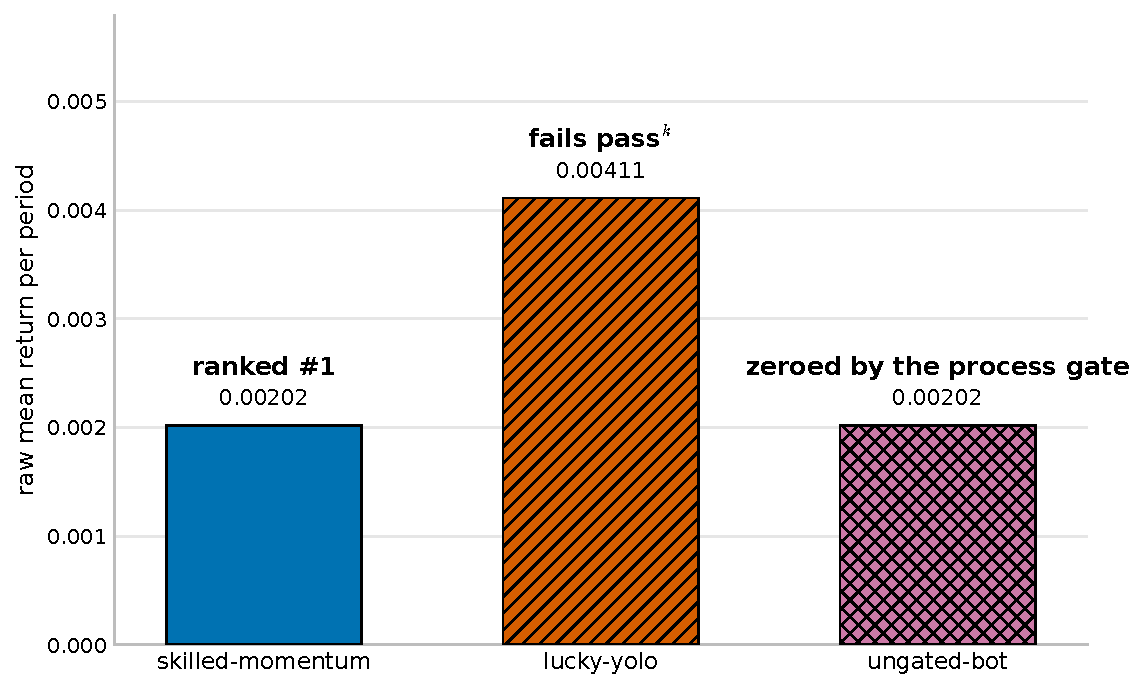
\includegraphics[width=\linewidth]{sharpebench-luck-demotion.pdf}
\caption{The agent with the highest raw return is refused and holds no rank.}
\label{fig:demotion}
\end{subfigure}

\vspace{0.8em}

\begin{subfigure}[b]{0.92\linewidth}
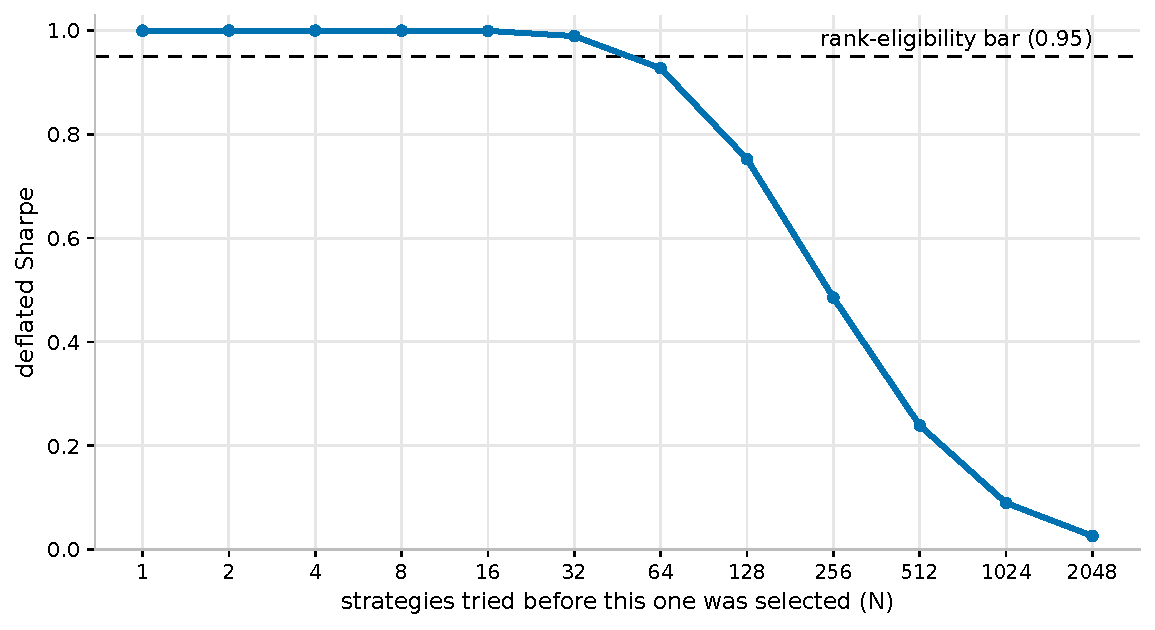
\includegraphics[width=\linewidth]{sharpebench-deflation-curve.pdf}
\caption{One track crosses the bar between 32 and 64 trials.}
\label{fig:deflation}
\end{subfigure}
\caption{Synthetic demonstrations, not evidence about any market. (a) Raw mean return per period of each agent and the gate outcome that decides its row, read from the kernel's golden score record \texttt{crates/sharpebench-core/golden/example\_submissions.scores.json} for \texttt{suites/example\_submissions.json}; hatching marks the two refused agents. (b) One synthetic track, per-period Sharpe $0.85$ over 150 periods with normal moments and a cross-trial dispersion of $0.30$ per period, deflated against a growing number of trials, with the dashed $0.95$ bar. It is computed by a Python transcription of the kernel's formulas (\texttt{paper/src/kernel\_stats.py}) that tests pin to the kernel's golden PSRs and to the worked example of \citet{bailey2014deflated}. Neither panel has a sampling spread: (a) plots fixed golden values and (b) is a deterministic function of its inputs.}
\end{figure}

\subsection{Finding 1: units of dispersion are a protocol trap}\label{sec:units}

The lesson generalizes to any scorer that combines literature constants with per-period statistics: the deflation literature states $\sigma_{\text{trials}}$ annualized, kernels compute Sharpe per period, and the conversion between them is a factor of $\sqrt{\text{periods per year}}$ that no self-consistency check will catch if it is dropped, for the reason \cref{sec:principles} gives. An earlier kernel omitted it.

The error surfaced when the first run of the full grid on the two original daily datasets produced zero rank-eligible agents in every one of the 128 cells. Buy-and-hold on US indices posted a PSR of $1.0000$ against zero and a bootstrap $p$ of $0.0005$, and scored a deflated Sharpe of exactly $0.0000$. Those values are mathematically compatible because PSR compares with zero while DSR compares with a search-adjusted threshold. Their coexistence nevertheless localized the refusal to that threshold rather than the return estimate and prompted the unit audit; the eight-attack self-audit stayed green throughout (\cref{sec:selfaudit}).

The default $\sigma_{\text{trials}} = 0.5$ is a free modelling prior. Earlier revisions of this paper and of the kernel's documentation attributed it to the annualized trial-dispersion example of \citet[pp.~102--103]{bailey2014deflated}, and the frozen record \texttt{paper/evidence/FINDING-units.md} still carries that earlier wording. The attribution is wrong in a way that matters: the example states the cross-trial \emph{variance}, $V[\{\widehat{SR}_n\}]=1/2$ annualized, and computes its threshold with the factor $\sqrt{1/(2\cdot 250)}$, so its dispersion is a standard deviation of $\sqrt{1/2}\approx 0.707$. \Cref{eq:deflation} uses $\sigma_{\text{trials}}$ as a standard deviation, so the shipped $0.5$ is less demanding than the cited example by a factor of $\sqrt{2}$: at $N=50$ it sets an annualized bar of $1.14$ where the example's dispersion would set $1.61$. A regression test reproduces the example's printed threshold of $0.1132$ per period and deflated Sharpe of $0.9004$ through the kernel's own entry points (\cref{app:commands}). The refusal results below survive the correction. $SR^{*}_{0}$ rises with $\sigma_{\text{trials}}$ and DSR falls as $SR^{*}_{0}$ rises, so a larger prior can only refuse more agents, and no agent clears the bar the smaller one sets; the onsets of the pass witness (\cref{sec:witness}), where $\passk$ rather than DSR binds, could only move later. The value itself is unchanged, because the published evidence is frozen and a prior is a stated choice, not a defect. Substituted per period into \cref{eq:deflation} at $N = 50$ it sets $SR^{*}_{0} = 1.14$ per period. \Cref{tab:units} converts that bar back into the annualized Sharpe an agent would need to reach it. On daily bars the requirement was an annualized Sharpe of $18$; on hourly bars, $106$. The three indices in \texttt{us-indices-1d} realize annualized price-return Sharpe ratios of $0.69$ (DJI), $0.79$ (SPX) and $0.87$ (IXIC) over their 2{,}512 daily returns, computed under the kernel's own convention (\cref{sec:stats}: price index levels without dividends, zero risk-free rate) by the script in \cref{app:commands}. The bar was unreachable, and it grew with the square root of the number of periods per year. A separate pre-floor experiment produced DSR $0.984$ weekly and $0.000$ daily from small field-measured dispersions; that contrast exposed instability in the measured-field estimate, not the configured-prior unit error. The current protocol records the source and applies the precommitted floor, and the current-floor results are reported separately below.

\begin{table}[t]
\centering
\small
\caption{The annualized Sharpe an agent had to exceed to reach the deflation benchmark at $N = 50$, for each prior as it was applied (per period) and each bar size. Each column annualizes the per-period bar by the square root of that column's periods per year: 8760 for 1h and 2190 for 4h, both on a 365-day year of continuous trading, 252 for 1d and 52 for 1w, the values in \cref{tab:data}. Kernel at v0.2.1, deliberately: this table documents that kernel's error. The $0.070$ row is the dispersion measured from the daily US indices field.}
\label{tab:units}
\setlength{\tabcolsep}{9pt}
\begin{tabular}{S[table-format=1.3] S[table-format=1.3] S[table-format=3.1] S[table-format=2.1] S[table-format=2.1] S[table-format=1.1]}
\toprule
{$\sigma_{\text{trials}}$ as applied} & {$SR^{*}_{0}$ per period} & {1h} & {4h} & {1d} & {1w} \\
\midrule
0.070 & 0.159 & 14.9 & 7.5 & 2.5 & 1.1 \\
0.200 & 0.455 & 42.6 & 21.3 & 7.2 & 3.3 \\
0.350 & 0.797 & 74.6 & 37.3 & 12.6 & 5.7 \\
0.500 & 1.138 & 106.5 & 53.3 & 18.1 & 8.2 \\
\bottomrule
\end{tabular}
\end{table}

The rival benchmarks of \cref{sec:related}, which rank LLM trading agents on return-based metrics over short windows, report annualized Sharpe without deflating for selection. This benchmark applied deflation with a prior in the wrong frequency units. These are different failures, an omitted multiple-testing correction and a dimensional miscalibration, rather than opposite unit errors. The latter is harder to notice because it produces a benchmark that appears strict. It also explains why the demonstration in \cref{sec:demo} had only ever been shown on synthetic inputs: those had per-period returns large enough to clear an annualized bar. The fix, shipped in v0.3.0, leaves the per-period kernel untouched and states the prior annualized with a periods-per-year field that converts it once at the point of use; \cref{app:simdata} gives the tests that pin it, which is the pinned unit-convention test the opening lesson calls for.

\subsection{Finding 2: the current defaults refuse on both edge and regime robustness}\label{sec:passk}

With the units corrected and the field-level defenses enabled, the full grid was rerun on all nine datasets. \Cref{tab:eligibility} reports the default configuration on each, with the dispersion source and annualized deflation bar printed for every row. Three sources are possible and the live evidence stamps which applied: the configured annualized $0.5$ prior, a value measured from the field, or a measured value raised to the annualized $0.5$ floor.

The measured path did not apply everywhere. Ranking measures the dispersion over the field's seed-averaged pooled streams after clone collapse, and it declines to measure when fewer than five votes survive that collapse. On five of the nine panels (both weekly panels, daily crypto, daily US indices and 4-hour crypto) the luck-floor agents merge into one cluster once their eight execution replicates are averaged, joined by buy-and-hold on three of the five, leaving three or four votes; those cells therefore fall back to the configured $0.5$ prior, at an annualized bar of $1.1382$. \Cref{sec:sybil} gives the cluster on each panel. Commodities measures a value below the floor and is raised to the same $0.5$, also $1.1382$. That stamp is frozen evidence: under the repaired simulator the same panel reconstructs too few finite-Sharpe streams to measure at all and would fall back to the configured prior instead (\cref{app:repairs}). Only daily FX, daily rates and hourly crypto measure above the floor, at annualized dispersions of $2.9985$, $1.5095$ and $12.0067$ and annualized bars of $6.8254$, $3.4362$ and $27.3309$. A regression test reproduces the clustering on those exact streams and asserts the vote counts the current engine supports on each panel (\cref{app:commands}); the merging itself is analyzed as a finding about the collapse threshold in \cref{sec:sybil}. Every stamp in this table also predates a later repair to the same measurement. The field on each panel includes \texttt{hold}, whose pooled track is identically zero and therefore has no Sharpe ratio, and the frozen kernel admitted it to the dispersion sample at the zero-variance sentinel of zero; the current kernel excludes it (\cref{sec:incentives}). Every measured and floored value printed here would therefore be computed from one fewer vote than the stamp records. The committed records carry each agent's deflated and probabilistic Sharpe but not its pooled Sharpe, so what the repaired measurement would give on these panels cannot be recovered from them, and none of it is estimated here (\cref{app:repairs}).

Weekly US buy-and-hold scores $0.1781$ and weekly crypto momentum $0.2406$, both far below $\beta=0.95$. The three measured panels show what the annualized bar reveals: the largest bar, $27.33$, occurs on the finest bars, and the smallest, $3.44$, on daily rates. Frequency alone does not order them, because daily FX sits at $6.83$ against daily rates at $3.44$ at identical periods per year, so the measured dispersion is panel-specific. The mechanism is cost drag: the luck floor's per-period cost bleed scales with the number of trades and not with $1/\sqrt{P}$, so the dispersion between a cost-bleeding random agent and a reference agent widens as bars get finer, and \cref{sec:external} confirms this directly by setting costs to zero, where the measured bar returns to the neighborhood of the precommitted floor on every one of the nine panels. That is the same dimensional mechanism Finding 1 generalizes, now visible on the measured side of \cref{eq:dispersion-floor} instead of the configured side. Measurement may make deflation stricter and can never take it below the precommitted prior.

No agent is eligible in any of the 72 agent-dataset verdicts, recorded as 4{,}608 records over the 576 dataset-configuration cells of the grid. At the shipped default, deflation and regime robustness refuse independently: every named reference agent is below the DSR bar, and every one also fails $\passk$. The reliability failure comes from windows rather than the narrow seed perturbations (\cref{sec:stats}): every frozen range contains at least one labeled bear window. The longer panels include the 2020 and 2022 drawdowns; the crypto 1h, 4h and 1d panels begin in 2023 and contain later drawdowns instead. The default mode requires a marginal per-run PSR of $0.90$ on every window. The long-only references in this field, buy-and-hold and momentum, fail that requirement in every window in which they lose money, because a negative realized Sharpe cannot clear a positive bar; \cref{tab:relative} shows the per-window pattern for every named agent. This is a statement about these agents on these windows, not about every long-only strategy. Four scopings bound this claim. It is sample-period-contingent: a different range can change the per-window verdict (\cref{sec:limitations} bounds this to the selected histories). The nine refusals are not nine independent confirmations: the resampled timeframes and co-moving symbols reduce to roughly five market panels with dependent histories. The refusal has low power: under serially independent normal returns the all-weather gate on six windows passes an agent with a true annualized Sharpe of $1$ only $1.4$ percent of the time on the daily geometry and $1.1$ percent on the weekly, passes one with a true Sharpe of $2$ about half the time, and reaches 95 percent only at $2.89$ and $3.03$ (\cref{sec:power}), so it cannot by itself distinguish no skill from realistic skill. And on three panels the deflation gate cannot discriminate within the field at all: on hourly crypto, daily FX and daily rates every one of the eight agents scores a deflated Sharpe of exactly zero at the default configuration, so each of those rows of \cref{tab:eligibility} is an eight-way tie and the printed agent is whichever tied record sorts first. \Cref{tab:dsr-mde} gives, for every panel, the minimum observed annualized Sharpe the DSR leg can admit at that panel's default bar; on those three panels it is $28.35$, $7.25$ and $3.85$. Only the synthetic witness of \cref{sec:witness} separates the gates and shows the conjunction attainable on a sampled grid.

The frozen evidence records carry no DSR interval, although the current kernel attaches a bootstrap interval to each score. \Cref{tab:eligibility}, \cref{tab:external}, \cref{tab:costsens} and \cref{tab:mandate} therefore print point estimates only, and a difference between two printed deflated Sharpes is not by itself evidence that the two differ. Adding the interval would require rescoring the frozen records, which this revision does not do.

\begin{table}[t]
\centering
\small
\caption{Default configuration ($\beta = 0.95$, host $N = 50$, field size eight) on all nine datasets. One row per dataset: the agent with the highest deflated Sharpe at this configuration. $^{\dagger}$An eight-way tie: every agent on that panel has a deflated Sharpe of exactly zero, so the printed agent, worst DD and $p_{\text{boot}}$ belong to whichever tied record sorted first, and the row names no leader. $^{\ddagger}$\texttt{hold} never trades, so its Sharpe ratio is undefined; its DSR is a value the frozen kernel computed for an undefined statistic, and the current kernel refuses it (\cref{sec:predicate}). \texttt{hold} is in the field on every row, not only the two it leads, and the frozen kernel also let it vote on the field-measured dispersion; the current kernel does not, so every \emph{measured} and \emph{floored} bar in this column would be recomputed from one fewer vote (\cref{app:repairs}). DSR is a point estimate; the frozen records carry no DSR interval (\cref{sec:passk}). Worst DD is the largest drawdown in any single window. $\sigma$ source is the dispersion source each record stamps: \emph{configured} is the annualized $0.5$ prior, applied because clone collapse over the seed-averaged streams left fewer than five dispersion votes; \emph{measured} is the field-measured value; \emph{floored} is a measured value raised to the annualized $0.5$ floor. Bar (ann.) is that cell's deflation benchmark $SR^{*}_{0}$ expressed as an annualized Sharpe. Eligible is the all-weather verdict of \cref{sec:passk}. Full per-agent records for all 512 configurations per dataset and the source-snapshot manifest are in \texttt{paper/evidence/}.}
\label{tab:eligibility}
\setlength{\tabcolsep}{3.5pt}
\footnotesize
\begin{tabular}{llS[table-format=1.3]S[table-format=1.3]S[table-format=1.4]lS[table-format=2.4]c}
\toprule
Dataset & Agent & {DSR} & {Worst DD} & {$p_{\text{boot}}$} & $\sigma$ source & {Bar (ann.)} & Eligible \\
\midrule
US indices 1w & buy-and-hold & 0.178 & 0.320 & 0.0015 & configured & 1.1382 & no \\
Crypto 1w & momentum & 0.241 & 0.563 & 0.0435 & configured & 1.1382 & no \\
Crypto 1d & buy-and-hold & 0.251 & 0.476 & 0.1219 & configured & 1.1382 & no \\
Commodities 1d & hold$^{\ddagger}$ & 0.000 & 0.000 & 1.0000 & floored & 1.1382 & no \\
US indices 1d & buy-and-hold & 0.156 & 0.336 & 0.0020 & configured & 1.1382 & no \\
Crypto 4h & buy-and-hold & 0.323 & 0.479 & 0.0735 & configured & 1.1382 & no \\
Crypto 1h & buy-and-hold$^{\dagger}$ & 0.000 & 0.490 & 0.0685 & measured & 27.3309 & no \\
FX 1d & hold$^{\dagger\ddagger}$ & 0.000 & 0.000 & 1.0000 & measured & 6.8254 & no \\
Rates 1d & buy-and-hold$^{\dagger}$ & 0.000 & 0.840 & 0.1754 & measured & 3.4362 & no \\
\bottomrule
\end{tabular}
\end{table}

The default mode does not ask only whether an agent has an edge. It requires every run's marginal PSR against zero to reach $0.90$ in every regime and under every execution seed; the conjunction is not itself a simultaneous 90-percent confidence statement. A regime-dependent edge such as equity beta correctly fails that question. On histories containing a downturn, the benchmark is declining to certify that owning the index is safe in a bear market, which it is not. Every return-based figure in the table is computed from price levels under a zero risk-free rate (\cref{sec:stats}).

\subsection{Finding 3: a weaker reliability gate admits nobody either}\label{sec:ablation}

Whether the reliability gate should mean profitable in every regime or never catastrophic in any regime is a design question (\cref{sec:predicate} states why the stricter verdict ships as the default), and the kernel was extended so that both are expressible from configuration and the ablation is reproducible (a third, benchmark-relative verdict is added in \cref{sec:relative}). The never-catastrophic preset sets the pass mode to any run and adds a per-run drawdown bound of 20 percent, with the edge tested on the pooled track. It is a weaker safety claim, and a test pins its cost: a synthetic agent with one high-return run and four noise runs is refused by the default only through $\passk$ and is admitted by the preset.

On the real datasets the preset admits nobody. The never-catastrophic verdict returns \emph{no} on all nine rows of \cref{tab:eligibility}, which is why that table prints one eligibility column and not two, and the worst-drawdown column supplies an additional refusal wherever a trading agent leads the row: seven of the nine rows breach the 20 percent bound outright. The two rows that print \texttt{hold} show a worst drawdown of $0.000$ because a cash agent never draws down; on commodities \texttt{hold} is the unique leader, and on daily FX it is only the first of eight tied records, so that row names no leader. The traded exposures on those same panels do breach the bound, daily-FX buy-and-hold at $0.199$ being the single exception in the grid, and both panels are refused by deflation and the bootstrap instead. The US index drew down 32 percent in its worst weekly window. Crypto buy-and-hold drew down between 48 and 67 percent across timeframes, and hourly momentum lost 99.3 percent of its value in a single window, the largest single-window loss in the grid. Crypto 4h buy-and-hold has the largest default reference-agent DSR at $0.3230$, still far below deflation, and that value holds only in the eight-agent field, whose clone collapse leaves too few votes to measure and falls back to the configured prior (\cref{sec:mandate}). Weekly crypto momentum is also refused on a 56 percent drawdown in one window and is the raw-return leader. On these datasets a 20 percent per-regime drawdown bound is not weaker than every-regime profitability; it is stricter for the unhedged exposure that crosses the cap.

One correction to how the per-run bound is naturally described. Under plain concatenation the usual description holds: drawdown is multiplicative, so a run's own drawdown never exceeds the pooled track's, because every within-run peak-to-trough pair is also a pooled pair. That is not the pooling this benchmark performs. Execution seeds are averaged \emph{within} a window before the pooled track is formed, and that averaging breaks the containment: a trough inside one seed can be cancelled by the opposite move in a sibling seed, so it never becomes a pooled pair at all. Two aligned runs $[0.1, -0.2]$ and $[-0.1, 0.2]$, scored as two execution seeds of a single window, average to $[0, 0]$, giving a pooled drawdown of $0.000$ against a worst-run drawdown of $0.200$. The pooled bound and the per-run bound are therefore \emph{independent} constraints rather than nested ones, neither implying the other, and the kernel retains both and checks each against the quantity it is written for. The per-run bound also bites, as already noted, when set below the pooled cap: a loose whole-track budget with a tight per-regime bound. The preset is configured that way, and a regression pins the anti-correlated-seed case beside the test that constructs the tight-per-regime one.

\subsection{Finding 4: the gates discriminate on a disciplined agent without alpha}\label{sec:riskmanaged}

The findings above show the gates refusing unhedged exposure, which leaves open whether they can distinguish anything finer. To probe that without inventing alpha, a risk-managed reference agent was added to the field: long the equal-weight basket only when it trades above its trailing mean, gross exposure scaled to an inverse-volatility target, and fully flat after a 10 percent drawdown with re-entry only on a fresh trend signal. It is textbook risk management and nothing more; every parameter is a documented default and none was tuned against the gate.

The result is a negative, and it narrows what the discrimination claim can be. Under corrected execution-seed pooling, weekly-US risk-managed does not clear the per-run PSR/reliability leg or the bootstrap. It remains process-clean and inside its 20-percent per-run drawdown bound, but is refused by deflation, bootstrap, and the applicable reliability verdict. The control therefore does not isolate deflation. What it shows is that documented risk controls improve drawdown on the weekly US panel without manufacturing an eligible statistical edge.

The result remains ineligible over the recorded trial-count sensitivity grid: every effective-$N$ setting is below the $0.95$ deflation bar, and the other refusing legs remain visible in the same records. On seven of the nine datasets the agent's worst-window drawdown is the smallest of any trading agent (\cref{fig:drawdowns}), so the discipline registers where it was designed to. What discipline does not manufacture is a deflation-surviving edge.

The two exceptions cut the other way. On hourly crypto the trend filter is whipsawed into an $87$ percent drawdown in one window, far worse than buy-and-hold's $49$, and on daily FX its $33$ percent trails buy-and-hold's $20$: the same rules that protect capital on daily and weekly equity bars amplify losses where the trend signal churns. Risk management is frequency-dependent, and a benchmark that scores per window is what makes that visible instead of averaged away.

Together with \cref{sec:passk} this shows the gates discriminate rather than blanket-refuse: unhedged beta fails on regime robustness, and discipline without edge, under the verdict that waives regime robustness, fails on deflation, each with the quantity that justifies it on the same row.

\begin{figure}[tbp]
\centering
\begin{subfigure}[b]{0.92\linewidth}
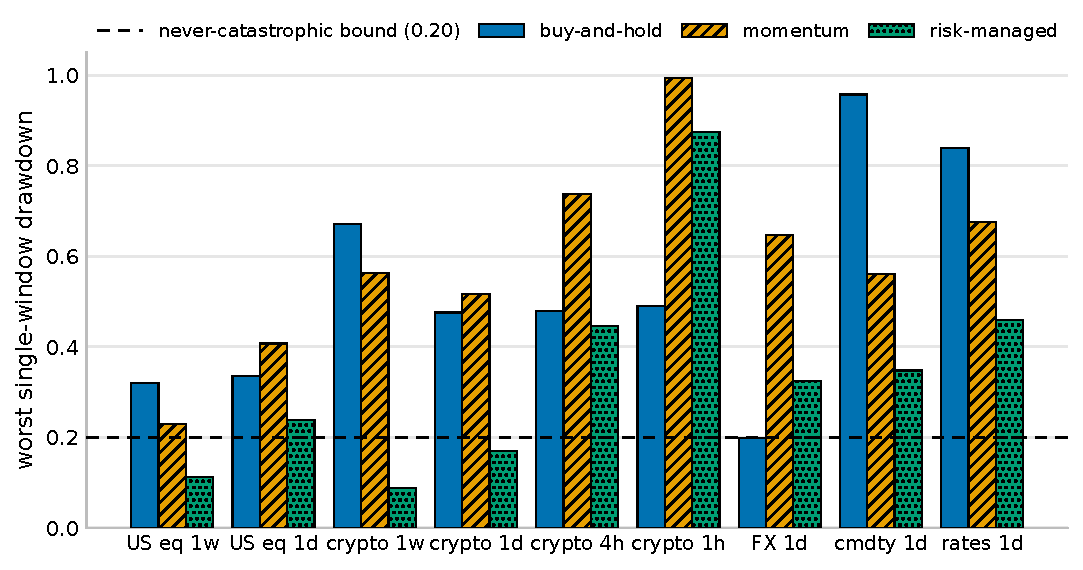
\includegraphics[width=\linewidth]{evidence-drawdowns.pdf}
\caption{The risk-managed agent has the smallest worst-window drawdown of any trading agent on seven of nine datasets.}
\label{fig:drawdowns}
\end{subfigure}

\vspace{0.8em}

\begin{subfigure}[b]{0.92\linewidth}
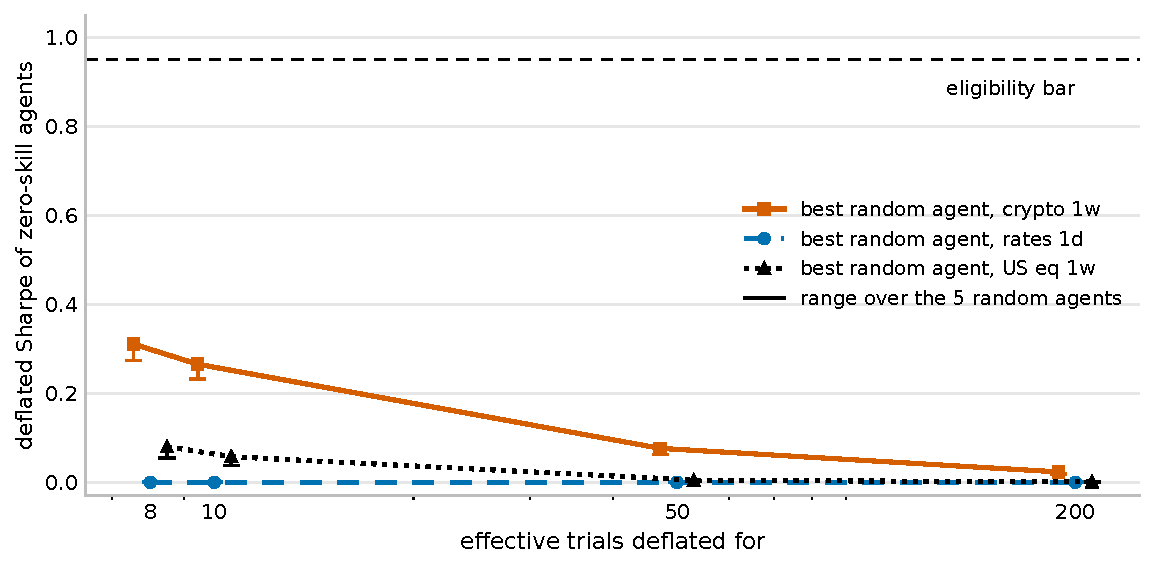
\includegraphics[width=\linewidth]{evidence-luck-deflation.pdf}
\caption{The best zero-skill agent's deflated Sharpe stays far below the bar at every effective trial count.}
\label{fig:luckdeflation}
\end{subfigure}
\caption{Computed from the committed evidence records by a committed script, in the Okabe-Ito palette. (a) Worst single-window drawdown of buy-and-hold, momentum and the risk-managed agent on each dataset, the agents distinguished by colour and by hatching; the dashed line is the 20 percent never-catastrophic bound. The risk-managed agent posts the smallest worst-window drawdown of any trading agent on seven of nine datasets, while both long-only references breach the bound almost everywhere and hourly momentum loses 99.3 percent in one window; the two exceptions, hourly crypto and daily FX, are where the trend filter itself whipsaws. Each bar is the maximum over all windows and seeds of a panel, and the records store only that maximum, so no spread is shown. (b) The operational DSR of the best of the five luck-floor agents against the effective trial count, on weekly crypto, daily rates and weekly US indices; each vertical bar runs down to the worst of the five at that count, and points that share a count are offset horizontally so their bars do not overprint. One agent's DSR is a pooled-track statistic with no interval in the frozen records. A host setting of one becomes eight because the submitted field has eight streams; the measured dispersion is also bounded below by the annualized prior. The curves therefore describe the shipped ranking path, not an unfloored diagnostic.}
\end{figure}

\subsection{Finding 5: externally specified rules, and what the cost profile moves}\label{sec:external}

Every entrant above was written for this repository, so a reader cannot yet separate a strict gate from a weak field. This subsection scores four trading rules whose specifications come from the published literature, and scores them under each of the three named cost profiles, which answers the cost-calibration limitation at the same time.

\paragraph{The rules.} \texttt{donchian-20-10} is the Donchian channel breakout at the Turtle System~1 parameters \citep{faith2007turtle}: enter long when the latest close exceeds the maximum of the prior 20 closes, exit to cash when it falls below the minimum of the prior 10. \texttt{bll-vma-1-50} is the variable-moving-average rule of \citet{brock1992simple}, long when the close is above its trailing 50-bar mean and flat otherwise, with no band. \texttt{faber-10m} is the ten-month simple-moving-average timing rule of \citet{faber2007quantitative}, converted to each dataset's own bar count. \texttt{rsi-14-wilder} is \citet{wilder1978new}'s RSI(14) with the 30/70 thresholds: enter long below 30, exit above 70, hold between. Each allocates $1/n_{\text{symbols}}$ to every symbol it is currently long, so gross exposure never exceeds one and the rules are comparable with the long-only references. We implemented each rule from its published statement and tuned no parameter here; the specification is external and the implementation is ours. Because every specification was published before any of the nine datasets begins, these four are the only entrants in the paper whose design is out of sample with respect to the data. \citet{sullivan1999datasnooping} applied White's Reality Check to a universe of 7{,}846 technical rules in filter, moving-average, support-and-resistance, channel-breakout and on-balance-volume families, which contains no RSI rule and no ten-month rule. In their sample the best rule survives the data-snooping adjustment, with an adjusted $p$ below $0.002$ in the full sample and in all four subperiods, and it does not survive in the 1987 to 1996 post-sample, where the adjusted $p$ is about $0.12$. The Reality Check corrects the best of a searched universe against a benchmark; \cref{eq:deflation} is a related but different correction, deflating one entrant's Sharpe for the number of trials behind it.

\paragraph{Evidence.} The field is the eight named agents (buy-and-hold, momentum, hold, the risk-managed agent of \cref{sec:riskmanaged}, and the four rules above) plus five luck-floor agents, thirteen in all, on the same nine datasets, the same window rule, the same eight execution seeds and the same default configuration, scored once per cost profile: 351 records. \Cref{tab:external} lists the four rules under the typical profile and \cref{tab:costsens} gives the cost sweep.

\paragraph{Result.} No record is rank-eligible and no record passes $\passk$, in any of the 351 cells, under any of the three cost profiles. The highest deflated Sharpe any entrant has reached anywhere in this paper is now an external one, \texttt{donchian-20-10} on daily crypto at $0.6534$ frictionless, $0.4155$ typical and $0.1185$ stressed, against the $0.95$ bar. That is above the $0.3230$ of \cref{sec:ablation} and still short of eligibility by a wide margin, and its block-bootstrap $p$ moves from $0.0425$ to $0.0655$ to $0.1499$ across the same three profiles. Removing every trading friction does not admit anybody, so the universal refusal of \cref{sec:passk} is not an artifact of the chosen cost calibration.

\paragraph{The cost profile moves the bar, not only the returns.} \Cref{tab:costsens} prints the annualized deflation benchmark on every cell, and it is the more interesting half of the sweep. Under the frictionless profile the measured field dispersion sits at or near the precommitted annualized floor on every one of the nine panels, so the bar is $1.1382$ on six of them and $1.2024$, $1.2576$ and $1.2825$ on daily, hourly and 4-hour crypto. Under the typical profile five panels rise well above that: hourly crypto to $27.5397$, daily FX to $6.7466$, 4-hour crypto to $5.2022$, daily rates to $3.2994$ and daily US indices to $1.9664$. Under the stressed profile those same five read $31.9269$, $10.1954$, $7.9760$, $2.8223$ and $1.8665$. This locates the mechanism \cref{sec:passk} attributes to sampling frequency: at zero cost the bar is near the floor at every bar size, so what widens the field's dispersion is the per-trade cost drag on the zero-skill agents, and frequency matters only because a finer bar buys more trades. Daily rates falls from $3.2994$ to $2.8223$ as costs rise, so the ordering is panel-specific even in cost.

\paragraph{The window geometry bounds the lookback a published rule may use.} The protocol's observation carries twenty trailing closes and each run starts fresh at its window boundary, so a rule needing $L$ closes emits no signal for the first $L-20$ bars of every window. \texttt{rsi-14-wilder} needs 15 and is never blind; \texttt{donchian-20-10} needs 21 and is blind for one bar; \texttt{bll-vma-1-50} needs 50 and is blind for 30. \texttt{faber-10m} needs 210 daily bars, 43 weekly, 1{,}825 at 4-hour and 7{,}300 at hourly, against windows of 408, 682, 677, 156, 78, 46, 990 and 3{,}990 bars, so it is blind for 190 of every 408-bar US daily window, for 23 of every 46-bar weekly crypto window, and for every bar of all six windows on daily crypto, 4-hour crypto and hourly crypto. The canonical twelve-month trend rules of the published literature are therefore not expressible on six of the nine panels at the shipped window rule, which is a property of the benchmark to fix, and \cref{sec:limitations} records it.

\paragraph{Field composition and comparability.} Adding four agents changes the field, so these deflated Sharpes are not the same statistic as \cref{tab:eligibility}'s. Where the effective bar is unchanged the numbers reproduce exactly: weekly US buy-and-hold is $0.1781$ and weekly crypto momentum is $0.2406$ in both tables, because the eight-agent field falls back to the configured $0.5$ prior there while the thirteen-agent field measures a value below the floor and is raised to the same $0.5$, giving an identical bar of $1.1382$ by two different routes. Where the wider field supplies enough surviving votes to measure above the floor, the bar moves: daily US indices, 4-hour crypto and daily crypto all stamp \emph{configured} in \cref{tab:eligibility} and \emph{measured} here, at typical-profile bars of $1.9664$, $5.2022$ and $1.4079$ against $1.1382$. Every record here serializes \texttt{trials\_sr\_std\_source} and the annualized bar beside the score, so the two tables reconcile cell by cell instead of merely differing. Two caveats attach to the measured half. The thirteen-agent field carries \texttt{hold} on every panel, and on the three crypto panels \texttt{faber-10m} posts an identically zero pooled track as well: the committed records give it a raw mean return of exactly zero and a worst-window drawdown of exactly zero, which together admit no other track. Both voted on the measured dispersion under the frozen kernel and neither would under the current one (\cref{sec:incentives}), so on the crypto panels two of the thirteen votes were cast by tracks with no Sharpe ratio. The eight-agent and nine-agent reconciliation is also a property of the frozen kernel: with \texttt{hold}'s vote withdrawn from both fields, the current engine takes the configured path on daily US indices, 4-hour crypto and weekly crypto in the nine-agent field as well as the eight-agent one (\cref{app:repairs}).

\paragraph{Command.} The producing command is listed in \cref{app:commands}. It writes one record per (dataset, cost profile, agent), 351 in all, each carrying the command, the rule's published source, the closes the rule requires, the blind-bar count, the dispersion source, the annualized bar and the full gate vector.

\begin{table}[t]
\centering
\footnotesize
\caption{The four externally specified rules on all nine frozen datasets under the typical cost profile, in a thirteen-agent field, at the default configuration ($\beta = 0.95$, host $N = 50$). Worst DD is the largest drawdown in any single window. Blind is the bars of every window in which the rule cannot form its signal, over the window length. No cell passes $\passk$ and no cell is eligible.}
\label{tab:external}
\setlength{\tabcolsep}{4pt}
\begin{tabular}{llS[table-format=1.4]S[table-format=1.3]S[table-format=1.4]rcc}
\toprule
Dataset & Rule & {DSR} & {Worst DD} & {$p_{\text{boot}}$} & Blind & $\passk$ & Eligible \\
\midrule
US indices 1d & \texttt{donchian-20-10} & 0.0000 & 0.119 & 0.0635 & 1/408 & no & no \\
US indices 1d & \texttt{bll-vma-1-50} & 0.0000 & 0.264 & 0.2189 & 30/408 & no & no \\
US indices 1d & \texttt{faber-10m} & 0.0002 & 0.101 & 0.0030 & 190/408 & no & no \\
US indices 1d & \texttt{rsi-14-wilder} & 0.0000 & 0.280 & 0.0240 & 0/408 & no & no \\
US indices 1w & \texttt{donchian-20-10} & 0.0247 & 0.153 & 0.0565 & 1/78 & no & no \\
US indices 1w & \texttt{bll-vma-1-50} & 0.0259 & 0.156 & 0.0695 & 30/78 & no & no \\
US indices 1w & \texttt{faber-10m} & 0.1254 & 0.156 & 0.0105 & 23/78 & no & no \\
US indices 1w & \texttt{rsi-14-wilder} & 0.1010 & 0.167 & 0.0185 & 0/78 & no & no \\
Crypto 1h & \texttt{donchian-20-10} & 0.0000 & 0.537 & 1.0000 & 1/3990 & no & no \\
Crypto 1h & \texttt{bll-vma-1-50} & 0.0000 & 0.623 & 1.0000 & 30/3990 & no & no \\
Crypto 1h & \texttt{faber-10m} & 0.0000 & 0.000 & 1.0000 & 3990/3990 & no & no \\
Crypto 1h & \texttt{rsi-14-wilder} & 0.0000 & 0.407 & 1.0000 & 0/3990 & no & no \\
Crypto 4h & \texttt{donchian-20-10} & 0.0000 & 0.292 & 0.2444 & 1/990 & no & no \\
Crypto 4h & \texttt{bll-vma-1-50} & 0.0000 & 0.367 & 0.4648 & 30/990 & no & no \\
Crypto 4h & \texttt{faber-10m} & 0.0000 & 0.000 & 1.0000 & 990/990 & no & no \\
Crypto 4h & \texttt{rsi-14-wilder} & 0.0000 & 0.374 & 0.2134 & 0/990 & no & no \\
Crypto 1d & \texttt{donchian-20-10} & 0.4155 & 0.165 & 0.0655 & 1/156 & no & no \\
Crypto 1d & \texttt{bll-vma-1-50} & 0.1807 & 0.264 & 0.1384 & 30/156 & no & no \\
Crypto 1d & \texttt{faber-10m} & 0.0121 & 0.000 & 1.0000 & 156/156 & no & no \\
Crypto 1d & \texttt{rsi-14-wilder} & 0.0213 & 0.246 & 0.3913 & 0/156 & no & no \\
Crypto 1w & \texttt{donchian-20-10} & 0.1221 & 0.432 & 0.0785 & 1/46 & no & no \\
Crypto 1w & \texttt{bll-vma-1-50} & 0.0011 & 0.427 & 1.0000 & 30/46 & no & no \\
Crypto 1w & \texttt{faber-10m} & 0.0021 & 0.434 & 1.0000 & 23/46 & no & no \\
Crypto 1w & \texttt{rsi-14-wilder} & 0.0333 & 0.146 & 0.1569 & 0/46 & no & no \\
FX 1d & \texttt{donchian-20-10} & 0.0000 & 0.170 & 1.0000 & 1/682 & no & no \\
FX 1d & \texttt{bll-vma-1-50} & 0.0000 & 0.226 & 1.0000 & 30/682 & no & no \\
FX 1d & \texttt{faber-10m} & 0.0000 & 0.151 & 1.0000 & 190/682 & no & no \\
FX 1d & \texttt{rsi-14-wilder} & 0.0000 & 0.161 & 1.0000 & 0/682 & no & no \\
Commodities 1d & \texttt{donchian-20-10} & 0.0007 & 0.342 & 0.0955 & 1/677 & no & no \\
Commodities 1d & \texttt{bll-vma-1-50} & 0.0000 & 0.586 & 1.0000 & 30/677 & no & no \\
Commodities 1d & \texttt{faber-10m} & 0.0000 & 0.466 & 1.0000 & 190/677 & no & no \\
Commodities 1d & \texttt{rsi-14-wilder} & 0.0000 & 0.940 & 0.1049 & 0/677 & no & no \\
Rates 1d & \texttt{donchian-20-10} & 0.0000 & 0.597 & 1.0000 & 1/682 & no & no \\
Rates 1d & \texttt{bll-vma-1-50} & 0.0000 & 0.611 & 1.0000 & 30/682 & no & no \\
Rates 1d & \texttt{faber-10m} & 0.0000 & 0.417 & 0.3478 & 190/682 & no & no \\
Rates 1d & \texttt{rsi-14-wilder} & 0.0000 & 0.822 & 0.3513 & 0/682 & no & no \\
\bottomrule
\end{tabular}
\end{table}

\begin{table}[t]
\centering
\footnotesize
\caption{Cost sensitivity across the three shipped profiles, thirteen-agent field, default configuration. Ext.\ is the highest deflated Sharpe among the four externally specified rules; Field is the highest in the whole thirteen-agent field; Bar is that cell's deflation benchmark expressed as an annualized Sharpe; every Bar in this table is field-measured, and the frozen kernel let \texttt{hold}, and on the three crypto panels \texttt{faber-10m}, vote on that measurement although neither has a Sharpe ratio, which the current kernel refuses (\cref{app:repairs}). Frictionless charges no fee, slippage, size-dependent rebalancing cost or financing; typical charges 2, 3, 50 and 5 basis points; stressed charges 10, 15, 150 and 20 with a per-step turnover cap of 10 percent of the agent's NAV. The rebalancing cost and the cap are measured against the agent's own NAV, not market volume (\cref{sec:simdata}). The stressed profile's two-bar decision delay is not applied, because the backtest driver consumes the cost model only. Zero cells are eligible and zero pass $\passk$ under every profile.}
\label{tab:costsens}
\setlength{\tabcolsep}{4pt}
\begin{tabular}{lS[table-format=1.4]S[table-format=1.4]S[table-format=2.4]S[table-format=1.4]S[table-format=1.4]S[table-format=2.4]S[table-format=1.4]S[table-format=1.4]S[table-format=2.4]}
\toprule
& \multicolumn{3}{c}{Frictionless} & \multicolumn{3}{c}{Typical} & \multicolumn{3}{c}{Stressed} \\
\cmidrule(lr){2-4}\cmidrule(lr){5-7}\cmidrule(lr){8-10}
Dataset & {Ext.} & {Field} & {Bar} & {Ext.} & {Field} & {Bar} & {Ext.} & {Field} & {Bar} \\
\midrule
US indices 1d & 0.2910 & 0.2910 & 1.1382 & 0.0002 & 0.0002 & 1.9664 & 0.0004 & 0.0004 & 1.8665 \\
US indices 1w & 0.1797 & 0.1918 & 1.1382 & 0.1254 & 0.1781 & 1.1382 & 0.0932 & 0.1550 & 1.1382 \\
Crypto 1h & 0.4315 & 0.6518 & 1.2576 & 0.0000 & 0.0000 & 27.5397 & 0.0000 & 0.0000 & 31.9269 \\
Crypto 4h & 0.5974 & 0.5974 & 1.2825 & 0.0000 & 0.0000 & 5.2022 & 0.0000 & 0.0000 & 7.9760 \\
Crypto 1d & 0.6534 & 0.6534 & 1.2024 & 0.4155 & 0.4155 & 1.4079 & 0.1185 & 0.1185 & 1.5695 \\
Crypto 1w & 0.1327 & 0.2935 & 1.1382 & 0.1221 & 0.2406 & 1.1382 & 0.0747 & 0.1451 & 1.1382 \\
FX 1d & 0.0000 & 0.0000 & 1.1382 & 0.0000 & 0.0000 & 6.7466 & 0.0000 & 0.0000 & 10.1954 \\
Commodities 1d & 0.0114 & 0.0114 & 1.1382 & 0.0007 & 0.0007 & 1.1382 & 0.0000 & 0.0000 & 1.1382 \\
Rates 1d & 0.0004 & 0.0007 & 1.1382 & 0.0000 & 0.0000 & 3.2994 & 0.0000 & 0.0000 & 2.8223 \\
\bottomrule
\end{tabular}
\end{table}

\paragraph*{The other two reliability verdicts.} Findings 2 and 3 fix the verdict and vary the agent. The next two subsections do the reverse: they hold the reference field fixed and vary the reliability question the host asks, first as a host configuration and then as a claim the submitter declares.

% Fragment: mandate-relative reliability verdict. \input from 05-experiments.tex after sec:riskmanaged.
% Evidence: paper/evidence/final/relative-mandate.jsonl (81 records, one per
% dataset x agent, produced by the command recorded on every record).

\subsection{A mandate-relative reliability verdict}\label{sec:relative}

The default reliability gate tests each run's Probabilistic Sharpe against zero: $\text{PSR}(r, 0) \ge 0.90$ in every window and under every execution seed. That is an all-weather absolute-return mandate, and \cref{sec:passk} showed its consequence on these histories: the index cannot pass on any range containing 2020 or 2022, and neither can anything that holds the index. The never-catastrophic verdict of \cref{sec:ablation} relaxes the \emph{aggregation} (one run is enough) and adds a drawdown bound. This section adds a third verdict that keeps the aggregation strict and changes the \emph{series under test}: each run is judged relative to owning the universe in that same window, which is the question most real mandates ask.

\paragraph{Definition.} Let $r_t(a, w, s)$ be agent $a$'s per-bar return in window $w$ under execution seed $s$, and let $b$ be the benchmark agent, buy-and-hold of the same universe. Under \texttt{PassMode::RelativeToBenchmark}, run $(w, s)$ of agent $a$ passes if and only if, for the excess series $e_t = r_t(a, w, s) - r_t(b, w, s)$,
\begin{equation}
\operatorname{std}(e) > 0 \quad\text{and}\quad \text{PSR}\big(e,\; \text{SR}^{\ast}_{\text{run}}\big) \ge 0.90,
\label{eq:relative}
\end{equation}
where $\text{SR}^{\ast}_{\text{run}}$ is the per-period benchmark the annualized \texttt{per\_run\_min\_annual\_sharpe} converts to, zero by default. The agent passes $\text{pass}^{k}$ if and only if every run passes, exactly as under the default. Every other gate (pooled deflated Sharpe, block bootstrap, process audit, drawdown mandate) is computed on the agent's own raw returns and is byte-identical under both verdicts; the relative verdict is a different reliability question, not a weaker set of gates.

Three properties of \cref{eq:relative} matter. First, the benchmark series is not an input: it is the run of the agent named \texttt{benchmark\_agent\_id} (default \texttt{buy-and-hold}) in the \emph{same field being ranked}, at the same position in the window-major layout, so it was produced from the same frozen bars, the same window, the same execution seed and the same cost model as the run it is subtracted from. Nothing is fetched from outside the field; a field without the named agent, or a misaligned cell, fails the run rather than falling back to the absolute test. Second, the benchmark cannot certify itself. Its own excess series is identically zero, and a zero-dispersion series is no evidence of outperformance: the kernel defines its Sharpe as $0$, so PSR returns $\Phi(0) = 0.5$ and the run fails any bar above one half; the explicit $\operatorname{std}(e) > 0$ clause makes the refusal unconditional, so an operator who lowered the bar to $0.5$ would still not admit buy-and-hold, and a clone of the benchmark under another name fails for the same reason. A run indistinguishable from the benchmark has no excess edge, and the verdict is a claim about excess edge in every window. Third, the reliability verdict is opt-in. \texttt{pass\_mode} deserializes to \texttt{all} from every existing config, so the benchmark-relative \emph{pass} predicate is not silently selected. The named benchmark also anchors the fixed aligned series for the reported RC/SPA/Romano--Wolf diagnostics; changing it can therefore change those diagnostics, while the default eligibility predicate remains unchanged. It is selected with \texttt{sharpebench run --pass-mode relative-to-benchmark [--benchmark-agent <id>]}, the same flags on \texttt{sharpebench score}, \texttt{ScoreConfig::relative\_to\_benchmark(id)} in Rust, or \texttt{relative\_to\_benchmark\_config(id)} in Python. \texttt{sharpebench\_core::per\_run\_passes} exposes the kernel's per-run vector so a report can say which windows passed, which is what the table below uses.

\paragraph{Evidence.} The same field as \cref{sec:riskmanaged} (buy-and-hold, momentum, hold, the risk-managed agent, and five luck-floor agents), the same window rule, the same eight execution seeds and the same cost model, on all nine frozen datasets, scored under the default verdict and under \cref{eq:relative} with buy-and-hold as the benchmark. Six windows times eight seeds is 48 cells per agent per dataset. \Cref{tab:relative} lists every named agent on every dataset; the 45 luck-floor records are summarized in the text because none of them changes.

\begin{table}[t]
\centering
\footnotesize
\caption{Per-window reliability under the default verdict (marginal PSR against zero at least $0.90$) and the relative verdict of \cref{eq:relative} (marginal PSR on excess over buy-and-hold at least $0.90$), all nine datasets. These are per-run thresholds, not simultaneous 90-percent confidence statements. Regimes are the six out-of-sample windows in order: U bull, D bear, C chop. A window is marked P when all eight seeds pass and a period otherwise. Cells is the number of the 48 (window, seed) cells that pass. Gained lists windows that pass relative and failed default; Lost the reverse. Every other gate statistic is identical under both verdicts. No agent is rank-eligible under either verdict on any dataset.}
\label{tab:relative}
\setlength{\tabcolsep}{4pt}
\begin{tabular}{llllrrllcc}
\toprule
Dataset & Agent & Regimes & Default / Relative & \multicolumn{2}{c}{Cells} & Gained & Lost & \multicolumn{2}{c}{Eligible} \\
 & & & (windows 0 to 5) & {def.} & {rel.} & & & def. & rel. \\
\midrule
US indices 1d & buy-and-hold & UUUDUU & \texttt{P...P.} / \texttt{......} & 16 & 0 & none & 0, 4 & no & no \\
US indices 1d & momentum & UUUDUU & \texttt{......} / \texttt{......} & 0 & 0 & none & none & no & no \\
US indices 1d & hold & UUUDUU & \texttt{......} / \texttt{......} & 0 & 0 & none & none & no & no \\
US indices 1d & risk-managed & UUUDUU & \texttt{......} / \texttt{......} & 0 & 0 & none & none & no & no \\
US indices 1w & buy-and-hold & UUUDUU & \texttt{..P.P.} / \texttt{......} & 16 & 0 & none & 2, 4 & no & no \\
US indices 1w & momentum & UUUDUU & \texttt{..P.P.} / \texttt{......} & 16 & 0 & none & 2, 4 & no & no \\
US indices 1w & hold & UUUDUU & \texttt{......} / \texttt{......} & 0 & 0 & none & none & no & no \\
US indices 1w & risk-managed & UUUDUU & \texttt{......} / \texttt{......} & 0 & 0 & none & none & no & no \\
Crypto 1h & buy-and-hold & UDUUDD & \texttt{P.P...} / \texttt{......} & 16 & 0 & none & 0, 2 & no & no \\
Crypto 1h & momentum & UDUUDD & \texttt{......} / \texttt{......} & 0 & 0 & none & none & no & no \\
Crypto 1h & hold & UDUUDD & \texttt{......} / \texttt{.....P} & 0 & 8 & 5 & none & no & no \\
Crypto 1h & risk-managed & UDUUDD & \texttt{......} / \texttt{......} & 0 & 0 & none & none & no & no \\
Crypto 4h & buy-and-hold & UDUUDD & \texttt{P.P...} / \texttt{......} & 16 & 0 & none & 0, 2 & no & no \\
Crypto 4h & momentum & UDUUDD & \texttt{......} / \texttt{......} & 0 & 0 & none & none & no & no \\
Crypto 4h & hold & UDUUDD & \texttt{......} / \texttt{.....P} & 0 & 8 & 5 & none & no & no \\
Crypto 4h & risk-managed & UDUUDD & \texttt{......} / \texttt{......} & 0 & 0 & none & none & no & no \\
Crypto 1d & buy-and-hold & UCUUDD & \texttt{P..P..} / \texttt{......} & 16 & 0 & none & 0, 3 & no & no \\
Crypto 1d & momentum & UCUUDD & \texttt{......} / \texttt{......} & 0 & 0 & none & none & no & no \\
Crypto 1d & hold & UCUUDD & \texttt{......} / \texttt{.....P} & 0 & 8 & 5 & none & no & no \\
Crypto 1d & risk-managed & UCUUDD & \texttt{P..P..} / \texttt{.....P} & 16 & 8 & 5 & 0, 3 & no & no \\
Crypto 1w & buy-and-hold & UDUUUD & \texttt{..PPP.} / \texttt{......} & 24 & 0 & none & 2, 3, 4 & no & no \\
Crypto 1w & momentum & UDUUUD & \texttt{P..P..} / \texttt{P....P} & 16 & 16 & 5 & 3 & no & no \\
Crypto 1w & hold & UDUUUD & \texttt{......} / \texttt{.....P} & 0 & 8 & 5 & none & no & no \\
Crypto 1w & risk-managed & UDUUUD & \texttt{......} / \texttt{.....P} & 0 & 8 & 5 & none & no & no \\
FX 1d & buy-and-hold & UDCUDU & \texttt{......} / \texttt{......} & 0 & 0 & none & none & no & no \\
FX 1d & momentum & UDCUDU & \texttt{......} / \texttt{......} & 0 & 0 & none & none & no & no \\
FX 1d & hold & UDCUDU & \texttt{......} / \texttt{.P....} & 0 & 8 & 1 & none & no & no \\
FX 1d & risk-managed & UDCUDU & \texttt{......} / \texttt{......} & 0 & 0 & none & none & no & no \\
Commodities 1d & buy-and-hold & UDUDUC & \texttt{..PP..} / \texttt{......} & 16 & 0 & none & 2, 3 & no & no \\
Commodities 1d & momentum & UDUDUC & \texttt{......} / \texttt{......} & 0 & 0 & none & none & no & no \\
Commodities 1d & hold & UDUDUC & \texttt{......} / \texttt{.P....} & 0 & 8 & 1 & none & no & no \\
Commodities 1d & risk-managed & UDUDUC & \texttt{......} / \texttt{.P....} & 0 & 8 & 1 & none & no & no \\
Rates 1d & buy-and-hold & DUUDUU & \texttt{....P.} / \texttt{......} & 8 & 0 & none & 4 & no & no \\
Rates 1d & momentum & DUUDUU & \texttt{......} / \texttt{......} & 0 & 0 & none & none & no & no \\
Rates 1d & hold & DUUDUU & \texttt{......} / \texttt{......} & 0 & 0 & none & none & no & no \\
Rates 1d & risk-managed & DUUDUU & \texttt{......} / \texttt{......} & 0 & 0 & none & none & no & no \\
\bottomrule
\end{tabular}
\end{table}

\paragraph{Result.} No agent becomes eligible under the relative verdict on any dataset, and no agent passes $\text{pass}^{k}$ under it: the best any agent manages is two of six windows (momentum on weekly crypto, 16 of 48 cells), and every other named agent passes at most one window. The 45 luck-floor records are unchanged in kind: at most 12 of 48 cells pass under the default and at most 3 under the relative verdict, no window passes on all eight seeds under either, and none is eligible. The ``nothing passes'' result is therefore not an artifact of the all-weather mandate: the mandate-relative verdict, which asks only for outperformance of the universe, refuses every entrant too.

What the relative verdict changes is \emph{which} windows pass, in the direction implied by the benchmark definition. Buy-and-hold loses every window it passed under the default (16 windows across the nine datasets) because it is now measured against itself, and gains none, by the zero-excess rule. Every window gained by any agent is a bear window: window 5 on the four crypto datasets (a bear window on each), window 1 on FX and commodities (bear on both). They are gained by the agents that were out of the market when the universe fell: \texttt{hold}, which holds cash and therefore has excess return equal to minus the index in every bar; the risk-managed agent, whose drawdown halt and trend filter took it flat; and momentum on weekly crypto, which closes to cash on a negative lookback and was flat for the closing bear. The default verdict cannot see this, because an agent that is flat in a bear window has zero raw return there and $\text{PSR}(0, 0) = 0.5$; the relative verdict sees it and credits it. Symmetrically, windows lost are bull windows in which the agent was profitable but did not beat the index: momentum's window 3 on weekly crypto, both of the risk-managed agent's windows on daily crypto, and all of momentum's windows on weekly US indices, where it tracks the index closely enough that its excess does not reach the marginal $0.90$ PSR threshold in either direction.

The two verdicts fail the same agents for complementary reasons, and neither reason is a benchmark defect. Under the default a long-only agent fails on the bear windows; under the relative verdict it fails on the bull windows, because it does not beat the market beta it is carrying. An agent that passes both would have to be both profitable and index-beating in every one of six regimes on eight seeds, which on these histories no reference agent is. The one structural caveat is stated rather than hidden: a cash agent has a positive excess series on every bear window, so on a range consisting only of bear windows the relative verdict would pass \texttt{hold} on $\text{pass}^{k}$. It would still not be eligible, because the pooled deflated Sharpe and the bootstrap are computed on its raw returns, which are zero, and that is the reason the relative mode changes the per-run series only and leaves the edge gates absolute. Being flat when the universe falls is reliability; it is not an edge.

\paragraph{Command.} The producing command is listed once in \cref{app:commands}. It writes one record per (dataset, agent), 81 in total, each carrying the command, the benchmark id, the per-window pass vectors under both verdicts, the windows gained and lost, the cell counts, and the gate statistics. The per-window vectors are produced by the kernel's own \texttt{per\_run\_passes}, not by a reimplementation.

% Fragment: the declared mandate at submission, included from 05-experiments.tex.
% Evidence: paper/evidence/final/mandate-declaration.jsonl (81 records, one per
% dataset x agent, produced by the command recorded on every record).

\subsection{A mandate declared at submission}\label{sec:mandate}

The design direction that \cref{sec:predicate} and the limitations state, a mandate declared at submission and certified against rather than selected by the host, is now built, and this section reports what it does to the reference field. A submission may carry a typed declaration, \texttt{DeclaredMandate}, with four variants: \texttt{AbsoluteReturn} (the shipped default verdict, restated); \texttt{RelativeTo\{benchmark\_id\}} (the benchmark-relative verdict of \cref{sec:relative} against a named agent); \texttt{DrawdownCapped\{max\_per\_run\_drawdown\}} (the never-catastrophic verdict of \cref{sec:ablation}, with the per-run bound declared by the submitter); and \texttt{OutperformBuyAndHold}, an explicitly excess-return mandate resolving to \texttt{RelativeTo} buy-and-hold. The former wire spelling \texttt{long\_only\_beta} remains readable for old artifacts but is not used for new declarations: outperformance is not a claim that an agent is beta-tracking or long-only. This release therefore implements declared \emph{verdict selection}, not certification that a portfolio fulfils a beta-tracking or other portfolio-purpose mandate; a defensible tracking predicate needs an independently specified benchmark, horizon and tolerance. The declaration is optional and defaults to absent.

\paragraph{Mechanism.} A declaration selects which reliability question $\text{pass}^{k}$ asks; it never relaxes a gate. Let $m_a$ be agent $a$'s declaration and $v(m_a)$ the verdict it resolves to. The agent's declared-mandate eligibility is the predicate of \cref{eq:eligible} with only the reliability conjunct exchanged:
\begin{equation}\label{eq:declared}
\text{eligible}_{v}(a) \;=\; \text{DSR} \ge \beta \;\wedge\; \text{pass}^{k}_{v} \;\wedge\; \text{process} \;\wedge\; p_{\text{boot}} < \alpha \;\wedge\; \text{mandate} \;\wedge\; \text{dd}_{v},
\end{equation}
where $\text{pass}^{k}_{v}$ uses the verdict's per-run series and aggregation (raw returns under every-run aggregation for \texttt{AbsoluteReturn}; excess over the named agent's same-cell run, every run, for the relative verdicts, with the zero-excess and missing-benchmark refusals of \cref{eq:relative} unchanged; raw returns under at-least-one aggregation for \texttt{DrawdownCapped}) and $\text{dd}_{v}$ is the declared per-run drawdown bound, vacuously true except under \texttt{DrawdownCapped}, where a bound outside $(0, 1]$ is a misdeclaration and fails. The deflated Sharpe, the bootstrap, the process audit and the host's drawdown mandate in \cref{eq:declared} are the same tests on the same raw returns as in \cref{eq:eligible}; a declaration cannot flip any of them, and a unit test asserts that raising the deflation bar refuses every declaration. Both verdicts are recorded on the score (\texttt{declared\_mandate}, \texttt{verdict\_applied}, \texttt{declared\_passed\_k}, \texttt{declared\_mandate\_eligible}), and the board row prints both clauses, so buy-and-hold's row reads ``ineligible under declared verdict (relative to buy-and-hold); host-board ineligible'' rather than a bare refusal.

\paragraph{Ranking.} Eligibility is reported per verdict and the verdicts never mix. The board sorts on \cref{eq:eligible} under the host's configuration, byte-identically with or without declarations, and the ordinal rank counts host-eligible agents only. Declared eligibility is an additional labeled column; among agents that are declared-eligible under the \emph{same} resolved verdict (the agent's mandate class: same variant, same benchmark id, same bound), a within-class ordinal orders them by deflated Sharpe. Agents under different mandates have answered different questions and are never ordered against each other, or against the all-weather board.

\paragraph{Evidence.} The field of \cref{sec:riskmanaged}, with buy-and-hold carrying the explicit \texttt{OutperformBuyAndHold} comparison, hold and momentum declaring \texttt{AbsoluteReturn}, and the risk-managed agent declaring \texttt{DrawdownCapped} at $0.20$. The five luck-floor agents are undeclared, and their 45 records are identical to the undeclared board. \Cref{tab:mandate} lists every declared agent on every dataset.

\begin{table}[t]
\centering
\footnotesize
\caption{Declared-mandate verdicts for every declared reference agent on all nine frozen datasets. OBH is \texttt{OutperformBuyAndHold} (relative to buy-and-hold), ABS is \texttt{AbsoluteReturn}, and DD .20 is \texttt{DrawdownCapped} at a per-run drawdown of $0.20$. DSR and $p_{\text{boot}}$ are pooled gates; pass$^k_v$ is the declared reliability leg; Meets is \cref{eq:declared}. None of the 36 declared agent--dataset cases meets its declared eligibility predicate.}
\label{tab:mandate}
\setlength{\tabcolsep}{3pt}
\begin{tabular}{lllrrcc}
\toprule
Dataset & Agent & Declared & DSR & $p_{\text{boot}}$ & pass$^k_v$ & Meets \\
\midrule
US indices 1d & buy-and-hold & OBH & 0.0000 & 0.0020 & no & no \\
US indices 1d & momentum & ABS & 0.0000 & 1.0000 & no & no \\
US indices 1d & hold & ABS & 0.0000 & 1.0000 & no & no \\
US indices 1d & risk-managed & DD .20 & 0.0000 & 1.0000 & no & no \\
US indices 1w & buy-and-hold & OBH & 0.1781 & 0.0015 & no & no \\
US indices 1w & momentum & ABS & 0.0264 & 0.0775 & no & no \\
US indices 1w & hold & ABS & 0.0003 & 1.0000 & no & no \\
US indices 1w & risk-managed & DD .20 & 0.0262 & 0.0715 & no & no \\
Crypto 1h & buy-and-hold & OBH & 0.0000 & 0.0685 & no & no \\
Crypto 1h & momentum & ABS & 0.0000 & 1.0000 & no & no \\
Crypto 1h & hold & ABS & 0.0000 & 1.0000 & no & no \\
Crypto 1h & risk-managed & DD .20 & 0.0000 & 1.0000 & no & no \\
Crypto 4h & buy-and-hold & OBH & 0.0000 & 0.0735 & no & no \\
Crypto 4h & momentum & ABS & 0.0000 & 1.0000 & no & no \\
Crypto 4h & hold & ABS & 0.0000 & 1.0000 & no & no \\
Crypto 4h & risk-managed & DD .20 & 0.0000 & 1.0000 & no & no \\
Crypto 1d & buy-and-hold & OBH & 0.2505 & 0.1219 & no & no \\
Crypto 1d & momentum & ABS & 0.0051 & 1.0000 & no & no \\
Crypto 1d & hold & ABS & 0.0343 & 1.0000 & no & no \\
Crypto 1d & risk-managed & DD .20 & 0.2118 & 0.1949 & yes & no \\
Crypto 1w & buy-and-hold & OBH & 0.1244 & 0.0795 & no & no \\
Crypto 1w & momentum & ABS & 0.2406 & 0.0435 & no & no \\
Crypto 1w & hold & ABS & 0.0044 & 1.0000 & no & no \\
Crypto 1w & risk-managed & DD .20 & 0.0057 & 0.4608 & no & no \\
FX 1d & buy-and-hold & OBH & 0.0000 & 1.0000 & no & no \\
FX 1d & momentum & ABS & 0.0000 & 1.0000 & no & no \\
FX 1d & hold & ABS & 0.0000 & 1.0000 & no & no \\
FX 1d & risk-managed & DD .20 & 0.0000 & 1.0000 & no & no \\
Commodities 1d & buy-and-hold & OBH & 0.0000 & 0.1244 & no & no \\
Commodities 1d & momentum & ABS & 0.0000 & 1.0000 & no & no \\
Commodities 1d & hold & ABS & 0.0000 & 1.0000 & no & no \\
Commodities 1d & risk-managed & DD .20 & 0.0000 & 1.0000 & no & no \\
Rates 1d & buy-and-hold & OBH & 0.0000 & 0.1754 & no & no \\
Rates 1d & momentum & ABS & 0.0000 & 1.0000 & no & no \\
Rates 1d & hold & ABS & 0.0000 & 1.0000 & no & no \\
Rates 1d & risk-managed & DD .20 & 0.0000 & 1.0000 & no & no \\
\bottomrule
\end{tabular}
\end{table}

\paragraph{Result.} No declared agent meets its declared eligibility predicate in any of the 36 declared agent--dataset cases. There is exactly one declared reliability pass: daily-crypto risk-managed. Its score is nevertheless refused by deflation ($\text{DSR}=0.2118$ against $\beta=0.95$) and the block bootstrap ($p_{\text{boot}}=0.1949$); its declared drawdown is within the $0.20$ bound (worst $0.170$). This is a more informative refusal than the host verdict because \cref{eq:declared} records which reliability question was asked without pretending that a declaration can waive an edge gate.

Buy-and-hold's \texttt{OutperformBuyAndHold} declaration is deliberately self-defeating: it resolves to ``beats buy-and-hold in every window'', while buy-and-hold \emph{is} that reference. Its excess series is identically zero, the zero-excess rule of \cref{eq:relative} refuses it in all $48$ cells on every dataset, and the same holds for any clone. The name now says exactly what the test asks; it does not misdescribe an excess-return test as a beta mandate. The mechanism still delivers legibility, ``ineligible under declared verdict (relative to buy-and-hold); host-board ineligible'' in place of a blanket refusal, but the reading is that declaration changes what the refusal \emph{says}, not whether it happens: on these histories and gates, stating the mandate admits nobody. Hold and momentum, whose declaration restates the default verdict, fail exactly as the default fails them, including hold's instructive case: a cash agent breaches nothing, and a zero series is evidence of no edge, not of safety worth certifying.

\paragraph{Command.}
\begin{verbatim}
cargo run --release -p sharpebench-harness \
  --example mandate_eval -- \
  paper/evidence/final/mandate-declaration.jsonl
\end{verbatim}
One record per (dataset, agent), 81 in total: 36 declared cases and 45 undeclared luck-floor records. Each carries the command, declaration, applied verdict and both eligibility columns. The declared columns are produced by the kernel's own \texttt{rank\_declared}, not by a reimplementation, and the host-verdict columns are byte-identical to the undeclared board.


% Fragment: the seed leg of pass^k under an opt-in execution-noise model.
% \input from 05-experiments.tex after the relative-mandate fragment, or cite
% from the Reliability paragraph of 03-benchmark.tex.
% Evidence: paper/evidence/final/seed-leg.jsonl (2646 records: 2592 per-run
% rows and 54 per-agent verdict rows, produced by the command recorded on
% every record: cargo run --release -p sharpebench-harness --example
% seed_leg_eval -- paper/evidence/final/seed-leg.jsonl).

\subsection{The seed leg under a richer execution-noise model}\label{sec:seedleg}

The Reliability paragraph of \cref{sec:benchmark} concedes that the seed leg of $\text{pass}^{k}$ is a narrow stability check: under the shipped cost model the eight execution seeds vary only the base slippage draw, a few basis points, so every refusal on the paper's grid is attributable to the window leg. This section adds an opt-in execution-noise model under which the seeds resample fills rather than basis points, re-runs the reference field under both profiles on three daily datasets, and answers two questions the concession leaves open: whether the seed leg ever becomes the refusing leg once execution is genuinely noisy, and how far per-seed Sharpes then disperse.

\paragraph{Definition.} Let an order at bar $t$ on symbol $i$ under execution seed $s$ request a change $\Delta$ in position value toward its target weight, after the liquidity cap. The model draws three uniforms $u_d, u_f, u_q \sim \mathcal{U}[0,1)$ from a SplitMix64 stream keyed on the triple, $R(s, t, i)$, so each quantity below is a pure function of $(s, t, i)$ and the base slippage draw of the default model is untouched. Three effects apply in order.
\begin{align}
\text{fill bar}\quad \tau &= t + \mathbb{1}[\,u_d < p_d\,],\label{eq:noise-delay}\\
\text{filled value}\quad \Delta_{\rm fill} &= \begin{cases}\varphi\,\Delta & \text{if } (1-\varphi)\,|\Delta| > \kappa\,\mathrm{NAV}_t,\\ \Delta & \text{otherwise,}\end{cases}\qquad \varphi = \varphi_{\min} + (1-\varphi_{\min})\,u_f,\label{eq:noise-partial}\\
\text{queue slippage}\quad s_q &= u_q\;\rho_t\;\min\!\Big(1,\ \frac{\pi}{\pi_{\rm ref}}\Big),\qquad \rho_t = \Big|\frac{c_t}{c_{t-1}} - 1\Big|,\quad \pi = \frac{|\Delta_{\rm fill}|}{\mathrm{NAV}_t}.\label{eq:noise-queue}
\end{align}
A fresh order uses \cref{eq:noise-delay}; a carried order fills at its scheduled bar without a second delay. A delayed order and the unfilled remainder $\Delta - \Delta_{\rm fill}$ of a partial fill (\cref{eq:noise-partial}) are carried to bar $t+1$ as an order for the same target weight, where they fill at bar $t+1$'s price before that bar's fresh orders; a fresh order on the same symbol supersedes the carried one, which is cancel-and-replace. The carry floor $\kappa$ makes a remainder worth less than $\kappa$ of NAV fill in full, so a carry drains in finitely many bars instead of shrinking geometrically forever. The queue term (\cref{eq:noise-queue}) is an adverse move of up to one bar's range, scaled linearly by participation up to $\pi_{\rm ref}$, and is added to the base seeded slippage and the square-root impact term before the fill price is formed, with the sign against the trade as before. The frozen datasets carry closes only, so $\rho_t$ is the close-to-close absolute move rather than a high-low range; it is a proxy, and \cref{eq:noise-queue} should be read as such. The shipped parameters are $p_d = 0.25$, $\varphi_{\min} = 0.5$, $\kappa = 10^{-3}$ and $\pi_{\rm ref} = 0.10$; none is calibrated to a venue, and the model is stylized by design.

The model is opt-in. \texttt{CostModel} gains a \texttt{noise: Option<ExecutionNoise>} field that deserializes to \texttt{None} from every existing configuration, and with \texttt{None} the fill arithmetic is the historical path in the same order, so the golden fixtures, the native/wasm parity tests and the evidence sweeps are byte-identical. \texttt{CostProfile::Realistic} resolves to the typical cost model with \texttt{ExecutionNoise::default()}. The carried orders live in the book state and are absent from a serialized snapshot when empty. Given $(s, t, i)$ every quantity is deterministic, and two runs under the same seed replay bit for bit.

\paragraph{Evidence.} The field of \cref{sec:riskmanaged} (buy-and-hold, momentum, hold, the risk-managed agent, and five luck-floor agents), the same window rule and the same eight execution seeds, on three daily datasets from three market panels: US indices (2513 bars, 3 symbols, six windows of 408 bars, regimes UUUDUU), crypto majors (1000 bars, 5 symbols, six windows of 156, regimes UCUUDD) and FX majors (4157 bars, 5 symbols, six windows of 682, regimes UDCUDU), scored under the default \texttt{ScoreConfig} for each dataset's periods per year. Every (window, seed) cell is tested against the per-run bar $\text{PSR}(r, 0) \ge 0.90$ through \texttt{sharpebench\_core::per\_run\_passes}, and each agent's verdict is decomposed by leg: a window whose eight sampled execution draws all fail is a \emph{window-leg} refusal, while a window with some sampled draws passing and some failing is a \emph{seed-leg} refusal. The decomposition is exhaustive for this eight-draw experiment: $\text{pass}^{k}$ holds if and only if neither leg refuses. For each (agent, window) the across-seed sample standard deviation of per-run annualized Sharpe is recorded, and for scale the across-window standard deviation of the per-window mean Sharpe. \Cref{tab:seedleg} lists the three trading reference agents on every dataset under both profiles; hold never trades, so both profiles give it identically zero returns, and the five luck-floor agents are summarized in the text because their seed dispersion is not an execution effect.

\begin{table}[t]
\centering
\footnotesize
\setlength{\tabcolsep}{3.5pt}
\caption{The seed leg of $\text{pass}^{k}$ under the default cost model and under \texttt{CostProfile::Realistic} (\cref{eq:noise-delay,eq:noise-partial,eq:noise-queue}), three daily datasets, eight seeds, six windows. Windows: P when all eight seeds pass the per-run bar, M when the seeds disagree, a period when all eight fail. Leg is the refusing leg. Seed std is the across-seed sample standard deviation of per-run annualized Sharpe, mean and maximum over the six windows; window std is the across-window standard deviation of the per-window mean Sharpe; mean SR is the mean per-run annualized Sharpe over the 48 cells. Closest fail is the highest PSR of any cell in an all-fail window, the nearest the window leg came to admitting a window. No agent passes $\text{pass}^{k}$ or is rank-eligible under either profile.}
\label{tab:seedleg}
\begin{tabular}{lllcccccrr}
\toprule
Dataset & Agent & Profile & Windows & Leg & \multicolumn{2}{c}{Seed std} & Window std & Mean SR & Closest fail \\
 & & & (0 to 5) & & mean & max & & & \\
\midrule
US indices 1d & buy-and-hold & default   & \texttt{P...P.} & windows & 0.0001 & 0.0002 & 0.8153 & $+0.984$ & 0.879 \\
US indices 1d & buy-and-hold & realistic & \texttt{P...P.} & windows & 0.0063 & 0.0092 & 0.8073 & $+0.966$ & 0.878 \\
US indices 1d & momentum     & default   & \texttt{......} & windows & 0.0025 & 0.0034 & 0.8849 & $-0.535$ & 0.723 \\
US indices 1d & momentum     & realistic & \texttt{......} & windows & 0.2210 & 0.3142 & 0.9366 & $-0.897$ & 0.674 \\
US indices 1d & risk-managed & default   & \texttt{......} & windows & 0.0019 & 0.0033 & 0.8637 & $-0.163$ & 0.861 \\
US indices 1d & risk-managed & realistic & \texttt{......} & windows & 0.2079 & 0.3446 & 0.8081 & $-0.801$ & 0.688 \\
\midrule
Crypto 1d     & buy-and-hold & default   & \texttt{P..P..} & windows & 0.0001 & 0.0001 & 1.7941 & $+0.716$ & 0.890 \\
Crypto 1d     & buy-and-hold & realistic & \texttt{P..P..} & windows & 0.0332 & 0.0536 & 1.8182 & $+0.679$ & 0.882 \\
Crypto 1d     & momentum     & default   & \texttt{......} & windows & 0.0019 & 0.0024 & 1.7856 & $-0.631$ & 0.898 \\
Crypto 1d     & momentum     & realistic & \texttt{......} & windows & 0.4354 & 0.5969 & 2.0989 & $-1.982$ & 0.687 \\
Crypto 1d     & risk-managed & default   & \texttt{P..P..} & windows & 0.0009 & 0.0013 & 1.6159 & $+0.574$ & 0.854 \\
Crypto 1d     & risk-managed & realistic & \texttt{P.....} & windows & 0.2579 & 0.4267 & 1.9319 & $-0.311$ & 0.785 \\
\midrule
FX majors 1d  & buy-and-hold & default   & \texttt{......} & windows & 0.0001 & 0.0001 & 0.6502 & $-0.070$ & 0.774 \\
FX majors 1d  & buy-and-hold & realistic & \texttt{......} & windows & 0.0074 & 0.0114 & 0.6442 & $-0.084$ & 0.775 \\
FX majors 1d  & momentum     & default   & \texttt{......} & windows & 0.0034 & 0.0044 & 0.8563 & $-4.142$ & 0.000 \\
FX majors 1d  & momentum     & realistic & \texttt{......} & windows & 0.1742 & 0.2265 & 0.7068 & $-4.031$ & 0.000 \\
FX majors 1d  & risk-managed & default   & \texttt{......} & windows & 0.0036 & 0.0109 & 0.5786 & $-1.917$ & 0.035 \\
FX majors 1d  & risk-managed & realistic & \texttt{......} & windows & 0.1263 & 0.1745 & 0.5882 & $-2.345$ & 0.033 \\
\bottomrule
\end{tabular}
\end{table}

\paragraph{Result.} The realistic profile makes the seed leg measure something, and it still never refuses. Pooled over the three trading agents and six windows, the across-seed standard deviation of per-run annualized Sharpe rises from $0.0015$, $0.0010$ and $0.0024$ under the default profile on US indices, crypto and FX to $0.1451$, $0.2422$ and $0.1026$ under the realistic profile, roughly two orders of magnitude; the largest single-window value is $0.5969$ (momentum on crypto). For the two agents that trade every bar the ratio of per-window seed dispersion to across-window dispersion is now between $0.13$ and $0.26$, where under the default it was below one percent; for buy-and-hold, which trades once and then drifts, the seed dispersion stays below $0.06$ because the model charges the fills, and buy-and-hold has almost none. The refusing leg is nevertheless \emph{windows} in all eighteen rows of \cref{tab:seedleg} under both profiles: for the reference agents not one window is mixed. The one change in a window verdict, risk-managed on crypto losing its second passing window (\texttt{P..P..} to \texttt{P.....}), is a whole-window shift, all eight seeds failing where all eight had passed, driven by the level effect of the noise on a rebalancing agent (mean Sharpe from $+0.574$ to $-0.311$), not by a seed-dependent verdict. The level effect is itself the largest visible consequence: momentum loses $0.36$, $1.35$ and gains $0.11$ of annualized Sharpe on the three datasets, risk-managed loses $0.64$, $0.88$ and $0.43$, and buy-and-hold loses $0.02$, $0.04$ and $0.01$. Among the luck-floor agents the two mixed windows that exist on the grid (luck-floor-00 and luck-floor-01 on crypto under the default profile, two and one of eight seeds passing window 0) disappear under the realistic profile, where every luck-floor window fails on all eight seeds; but the luck floor's seed dispersion of $0.14$ to $0.31$ under the default profile is a policy effect, each \texttt{RandomAgent} being re-seeded per run, and says nothing about execution noise.

\paragraph{Interpretation.} The seed leg does not refuse because the per-window PSRs of these agents sit far from the bar on both sides. The Closest fail column shows the nearest any all-fail window came to $0.90$: $0.898$ for momentum on crypto under the default, where the across-seed PSR range on that window was $0.0014$, and $0.687$ under the realistic profile, where the range had grown to $0.464$ but the level had moved away from the bar faster than the dispersion grew. On the passing side the tightest margin is buy-and-hold's second passing window on crypto, whose lowest seed PSR is $0.9012$ under the default and $0.9086$ under the realistic profile, with the across-seed PSR range on that window at $0.0001$ and $0.0402$; the realistic profile brings the seed range to the same order as that margin, and the window stays unanimous by roughly one range width. That is the honest reading: under the shipped model the seed leg cannot flip a window because the seeds barely move the PSR, and under the realistic model it could flip a window that sits within a few hundredths of the bar, but on this grid no window does. The paper's statement that every refusal is a window-leg refusal therefore survives the richer noise model on three panels, with the qualification that the seed leg is now a live test rather than a formality.

Three caveats bound the claim. The noise model is stylized: its four parameters are set by hand, the range proxy is close-to-close because the datasets carry no high or low, and carried orders fill at the next close, so the model has the structure of delay, partial fill and queue loss but not the magnitudes of any particular venue. The across-seed standard deviations are estimated from eight seeds, for which the relative standard error of a sample standard deviation is about $27$ percent under an IID normal approximation (\cref{sec:incentives}), so the two-orders-of-magnitude contrast is robust and the third digit is not. And three daily datasets from three panels are enough to show that the seed leg can be made to measure execution and still not be the refusing leg for these agents, not enough to say it never is; an agent whose per-window Sharpe sits near the bar, which none of the author-written references does, is exactly the case in which the realistic seed leg would decide, and that is the case the arena is meant to see.


\subsection{Robustness under perturbation}\label{sec:perturb}

The self-audit's adversarial-input attack records its own limit: fragility that no submitted run exercises is invisible to a deterministic kernel. The harness now generates perturbed datasets whose bar-to-bar moves are nudged within the empirical range of the original series, a constraint asserted per bar, so every perturbed path is one the market could have printed. Scoring a field across perturbations reports each agent's spread between best and worst per-run PSR. On weekly US indices the committed report gives a spread of $0.0928$ for the risk-managed agent and $0.0534$ for buy-and-hold. Both are far larger than the pre-repair pooled figures, because averaging aligned execution seeds within a window removes the replicate noise a concatenated track averaged over, leaving a per-run PSR that responds to the perturbation. They are also of the same order as each other, so the committed report on this panel separates nothing: a factor of $1.7$ between two agents, neither of which is designed to be fragile, is not a diagnosis. The separation the diagnostic exists to produce is pinned by a unit test on synthetic data rather than by the committed report: a deliberately fragile agent that latches onto an exact price value shows more than twice buy-and-hold's spread, and the test (\texttt{cargo test -p sharpebench-harness perturb}, \cref{app:commands}) asserts that separation on every commit. On the real panel the diagnostic reports spreads; it is the synthetic test, not the committed report, that establishes the separation is detectable at all.

\subsection{A synthetic pass witness: the acceptance region is nonempty}\label{sec:witness}

Universal refusal is compatible with two hypotheses: the gates discriminate, or the eligibility conjunction is jointly unsatisfiable at the shipped defaults on these histories. The reference field cannot separate them, so a witness was constructed. A family of synthetic agents with a controlled injected edge, per-period returns drawn with true Sharpe $s$ by construction, was scored through the shipped default configuration on two window geometries matching the real datasets' window rule: six 77-bar windows at 52 periods per year, and six 409-bar windows at 252 periods per year. Before the edge sweep, a separate five-agent zero-edge calibration field fixes the measured dispersion (including its precommitted floor); that value is then serialized as an exogenous fixed bar for every witness point. The witness and its display controls therefore cannot set their own DSR threshold.

The acceptance region is nonempty (\cref{fig:witness}). Every figure in this paragraph comes from a single common-random-number draw of the witness returns, so it describes where that draw first admits the witness, not where the boundary lies in expectation. On the weekly geometry the witness becomes rank-eligible at an injected per-period Sharpe of $0.40$ (annualized $2.88$); on the daily geometry at $0.25$ per period (annualized $3.97$). Under the exogenously calibrated bar, $\passk$ is the binding gate on both geometries. DSR clears from the first nonzero sampled edge, $s = 0.05$, on the daily geometry ($1.0000$) and from $s = 0.10$ on the weekly geometry ($0.9984$, after $0.5097$ at $s = 0.05$), and reaches $1.0000$ from $s = 0.15$ upward on both; what moves the onset is the per-run leg, which requires every one of 48 window-times-seed runs to clear a marginal per-run PSR of $0.90$ and does not do so until $0.25$ daily and $0.40$ weekly. The weekly onset is the later of the two because its windows are 77 bars against 409. Both onsets are grid points on a sweep in steps of $0.05$ under that one draw, so within the draw eligibility first appears in $(0.35, 0.40]$ weekly and $(0.20, 0.25]$ daily. Across draws the onset is a random quantity. The sweep has not been replicated over independent noise draws, so the location of the boundary carries sampling uncertainty that this paper does not quantify. \Cref{sec:power} bounds how wide that uncertainty can be under serially independent normal returns. The witness's $\passk$ leg asks all 48 of its independent runs to pass, and under those assumptions that layout passes 5 percent of the time at an annualized true Sharpe of $2.22$ and 95 percent at $3.42$ on the daily geometry, and at $2.35$ and $3.60$ on the weekly geometry, a band of roughly 1.5 witness grid steps daily and 3.5 weekly. One draw's onset can therefore fall a grid step or more away from where that leg passes with high probability, more plausibly on the weekly geometry. Replication over independent draws is planned, not done. One earlier draw is on record: the frozen predecessor of this field, generated under the collided seeds described in \cref{app:repairs}, placed both onsets one grid step lower, at $0.35$ weekly and $0.20$ daily, under the same floored bar. These boundaries reflect the $\sqrt{n-1}$ behavior of \cref{eq:psr}. The witness turns the paper's central negative into a calibration and is the benchmark's headroom statement: the risk here is not saturation but unsatisfiability, and on window lengths of one to two years the shipped defaults first admit the sampled witness in this draw between annualized Sharpe $2.9$ and $4$. An operator who wants a lower bar must lengthen the windows or lower the per-run bar explicitly in configuration. Because the producer aborts if the deflated Sharpe decreases or eligibility closes after opening, ``boundary'' here means the first point of a monotone sampled acceptance set and not a local crossing between unrelated draws.

\begin{figure}[t]
\centering
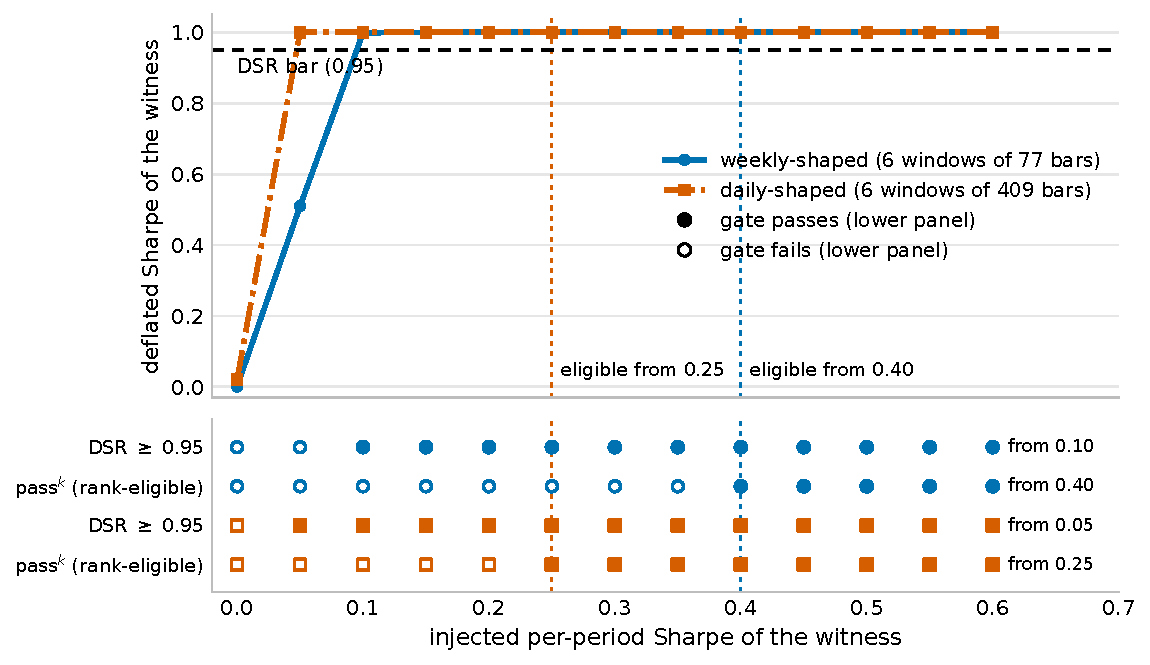
\includegraphics[width=\linewidth]{evidence-pass-witness.pdf}
\caption{The pass-witness boundary in a single common-random-number draw, computed from the committed witness records by the evidence-figure script. The records hold one draw and no replicate, so no spread is shown, and the onsets carry sampling uncertainty this draw does not quantify. Weekly geometry: solid line with circles; daily geometry: dash-dot line with squares. Top: the witness's deflated Sharpe against its injected per-period Sharpe on the two window geometries, with the $0.95$ bar; the dotted verticals mark the onset of rank eligibility, $0.40$ on the weekly geometry and $0.25$ on the daily. Bottom: the two gate outcomes at every injected edge, filled where the gate passes and hollow where it fails. DSR clears from the first nonzero sampled edge, $s = 0.05$, on the daily geometry and from $s = 0.10$ on the weekly, so $\passk$ is the gate that binds at both onsets: it turns on at $0.25$ daily and $0.40$ weekly, which are the onsets marked above.}
\label{fig:witness}
\end{figure}

\subsection{The falsification leg}\label{sec:falsify}

A benchmark whose gates are strict can still be wrong in the other direction, by rewarding noise, so the luck floor is scored everywhere. The original floor was fully invested in random weights each period, and on a one-symbol universe the normalized weight is deterministically $1.0$: on the rates dataset all five ``random'' agents were bit-identical clones of buy-and-hold, sharing its raw return to the last digit, so that construction was not a control there. The floor now draws a random gross exposure per period on one-symbol universes (flat half the time, otherwise a uniform long weight), a regression test pins the non-degeneracy, and the rates evidence is generated under that construction; all multi-symbol datasets reproduce byte-identically, since their path is untouched.

Under the corrected floor, on every dataset the luck floor's best agent has a lower raw return than the best reference agent, with zero exceptions in the nine dataset-timeframe combinations. The operational path also applies the precommitted annualized dispersion floor and the observable field-size floor before deflation.

The grid's nominal $N=1$ corner no longer disables deflation. Ranking observes eight submitted streams, so \cref{eq:effective-n} raises the effective count to eight before adding any declared search history. On weekly crypto the best random agent then scores $0.3105$ at host $N=1$, where \cref{eq:effective-n} has already raised the effective count to eight, and $0.0762$ at host $N=50$; on weekly US indices the corresponding values are $0.0800$ and $0.0044$. Neither is eligible, and $\passk$ refuses them independently. On the corrected rates floor no random agent scores above zero: genuinely random exposure on the yield series loses money after costs. The degenerate score the earlier one-symbol construction produced there is recorded with the other protocol corrections in \cref{sec:limitations}. \Cref{fig:luckdeflation} plots that corner as a curve: the best zero-skill agent's operational DSR against the effective trial count, entering at the eight-stream floor and decaying monotonically, so no host setting on this grid recovers an eligible zero-skill score. The counterfactual $N=1$ score remains useful only through the direct single-agent scoring API, where it is explicitly not a ranked field; a leaderboard cannot make its submitted alternatives disappear by declaring one trial.

% Thousand-agent extension to the falsification leg. Evidence:
% paper/evidence/final/luck-floor-1000.jsonl, produced by the command in
% Appendix A.

\subsection{The thousand-agent luck floor}\label{sec:luck1000}

The opening image is a thousand random agents; the original evidence floor used five seeded agents per dataset, which located the floor but not its extreme tail. We therefore ran 1{,}000 distinct seeds on \texttt{us-indices-1d} and \texttt{crypto-majors-1d}, under the same windows, eight execution seeds and costs as the evidence sweep. The first five return streams are byte-identical to the shipped floor, but all scores are recomputed with the observable 1{,}000-entry trial footprint. Three scores distinguish an operational result from a diagnostic: the configured annualized prior, the raw field-measured dispersion with its safety floor deliberately disabled, and that measured dispersion after applying the shipped floor. The raw diagnostic on daily crypto reaches $0.0302$, versus $0.00751$ among the first five streams in the same 1{,}000-entry context. The measured annualized field dispersion is only $0.0455$, so applying the precommitted $0.5$ floor drives the operational maximum to zero; the configured-prior path is also zero. None of the 2{,}000 agent-dataset cells is eligible, and no random agent beats the best reference agent on raw return on either dataset. The diagnostic tail moves; the operational conclusion does not.

\begin{figure}[t]
\centering
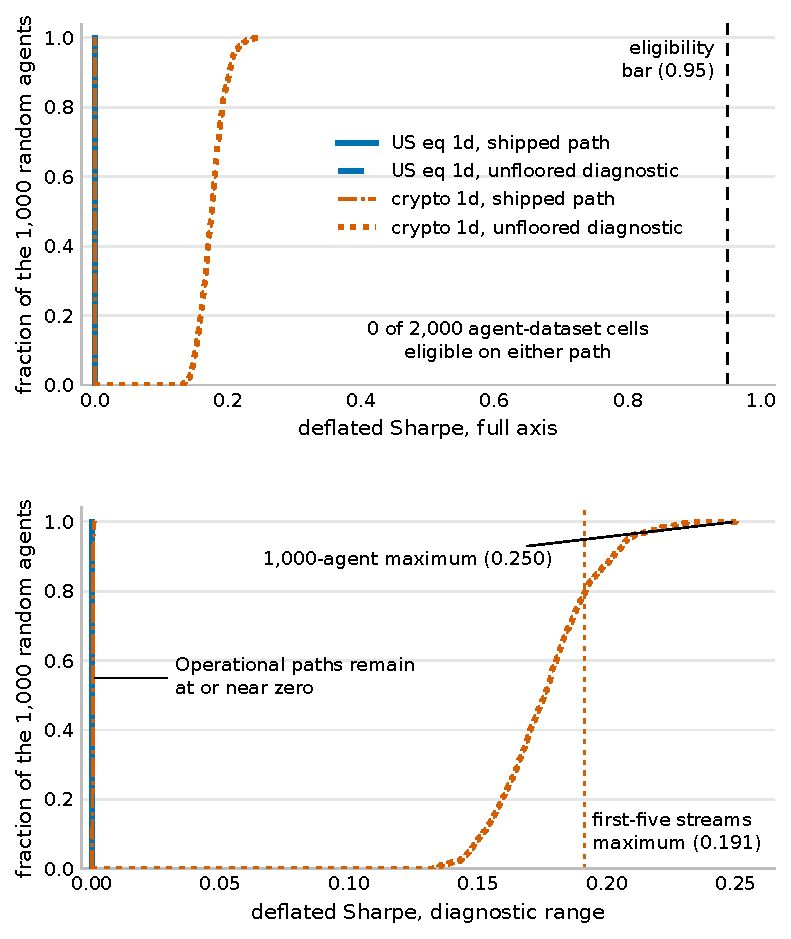
\includegraphics[width=\linewidth]{evidence-luck-floor-1000.pdf}
\caption{Empirical distributions over the 1{,}000 random agents on each daily dataset, all scored at the observable 1{,}000-trial footprint. The solid operational curves apply the shipped annualized dispersion floor; the dashed curves are deliberately unfloored diagnostics. The daily-crypto diagnostic reaches $0.0302$, but that value is not used by ranking. Left: the full axis with the $\beta=0.95$ bar. Right: the diagnostic range. No agent is eligible, and both operational maxima are zero.}
\label{fig:luck1000}
\end{figure}


% Power of the default gates: a protocol property, not a measurement. \input from
% 05-experiments.tex immediately before sec:claims.
% Evidence: paper/evidence/final/power-curve.jsonl, written by
% paper/src/make-power-curve.py from the committed default-cell bars. No agent,
% simulator run, market data or model is involved.

\subsection{What the default gates can detect}\label{sec:power}

Every verdict this section reports on a real panel is a refusal, and a refusal tells a reader something only if the gate could have admitted a skilled agent. This subsection asks how often the shipped gates admit an agent whose skill is known. The answer is a property of the gates' statistics under stated assumptions. It is a new calculation added in this revision, not a measurement of any agent and not a correction of frozen evidence: no agent, simulator run, market data or model is involved, it reads only the committed deflation bars, and no number reported elsewhere in this paper changes.

\paragraph{Assumptions and method.} Per-period returns are serially independent and normal with a known true Sharpe ratio, the same in every window. Two legs of \cref{eq:eligible} are modelled through the kernel's own formulas. The regime-robustness leg, $\passk$ in its default mode, passes when each of six windows reaches a per-run PSR of at least $0.90$ against zero under \cref{eq:psr}: the sample Sharpe over the $n-1$ standard deviation, population-normalized skewness and non-excess kurtosis, the standard error at the observed Sharpe with $\sqrt{n-1}$, and the kernel's normal CDF. On the real panels a window's eight execution seeds differ only by slippage (\cref{sec:stats}), so one run per window is modelled. The deflation leg passes when the pooled six-window track reaches DSR $0.95$ against the panel's committed per-period bar in the default cell of \cref{tab:eligibility}, held fixed. The bootstrap, process and mandate legs are not modelled. They can only refuse more, so the true Sharpe at which the full predicate reaches a given pass probability is at least the value printed below for the two legs together.

Skewness and kurtosis do not change when a constant is added to a series, and for fixed moments the observed Sharpe ratios that pass \cref{eq:psr} form a half-line above one threshold, so each simulated window has one true Sharpe at and above which it passes, solved in closed form. A leg therefore passes at true Sharpe $s$ exactly when $s$ reaches the largest threshold the leg involves. One set of draws then gives the whole curve: the pass probability at every $s$ is the empirical distribution function of those thresholds, and the 5 and 95 percent points are its quantiles, with no interpolation over a grid of Sharpe levels. The producer draws 200{,}000 replications per window geometry from NumPy's PCG64 generator under seed $20260915$, split into 64 fixed seeded chunks, and records every point's binomial standard error and, for every crossing, a 95 percent order-statistic band under the normal approximation to the binomial. A regression test checks the closed-form thresholds against the kernel formula evaluated on the shifted series themselves. The commands are
\begin{verbatim}
python paper/src/make-power-curve.py compute --jobs 32
python paper/src/make-power-curve.py figure
\end{verbatim}
The first writes \texttt{paper/evidence/final/power-curve.jsonl}; its bytes do not depend on the worker count, and it took $313.2$ seconds in one process and $53.6$ seconds with 32 worker processes on the machine described above. The second draws \cref{fig:power} from the committed file. Run without an argument, the script does both in one process.

\paragraph{The regime-robustness leg.} On the daily geometry of \cref{fig:power}, the six 408-bar windows of US indices 1d at 252 periods per year, $\passk$ passes $1.4$ percent of the time at a true annualized Sharpe of $1$ and $51.6$ percent at $2$. It reaches 5 percent at $1.23$ and 95 percent at $2.89$. On the weekly geometry, six 77-bar windows at 52 periods per year as in the synthetic witness, the same four values are $1.1$ percent, $43.8$ percent, $1.29$ and $3.03$. The gate therefore moves from rarely passing to reliably passing across $1.66$ annualized Sharpe units on the daily geometry and $1.75$ on the weekly. At a true Sharpe of zero no replication passed on either geometry. Every point of the two curves has a standard error of at most $0.0012$, and the 95 percent band around each of their crossings extends less than $0.01$ to either side. The US indices 1w panel's windows hold 78 bars rather than 77; its $\passk$ leg, recorded in the same evidence file, crosses 5 and 95 percent within $0.02$ of the weekly curve.

\paragraph{The deflation leg, and both legs together.} \Cref{tab:dsr-mde} extends the calculation to all nine default panels, with each panel's own window length, committed bar and pooled length. Its DSR minimum is derived rather than simulated. Under normal moments DSR against a per-period bar $b$ over a pooled track of $n$ returns reaches $0.95$ when $(u-b)\sqrt{n-1} = z\sqrt{1+u^{2}/2}$, where $u$ is the observed per-period Sharpe and $z = 1.6449$ is the point at which the kernel's normal CDF reaches $0.95$. Squaring gives $(n-1-z^{2}/2)\,u^{2} - 2b(n-1)\,u + b^{2}(n-1) - z^{2} = 0$. Its left side equals $-z^{2}(1+b^{2}/2) < 0$ at $u = b$, so $b$ lies between the two roots and the smallest admissible per-period Sharpe is the larger root; the table annualizes it by $\sqrt{P}$, with $P$ periods per year. That minimum is a normal-moment value, not an absolute one. A two-point return distribution has kurtosis equal to one plus its squared skewness, and with skewness $2/u$ it drives the radicand of \cref{eq:psr} toward zero, so for a suitably shaped track the requirement falls toward the bar itself: the committed bar is the lower limit. On the six panels whose bar is the annualized $0.5$ prior or floor, the DSR minimum runs from $1.55$ on commodities to $2.17$ on daily crypto. On the three measured panels it lies $0.41$ to $1.02$ above the bar, at $28.35$ on hourly crypto, $7.25$ on daily FX and $3.85$ on daily rates.

The table's remaining columns are simulated, both legs on the same draws, so the both-legs columns are the exact conjunction under the assumptions. On the six panels at the $1.1382$ bar, $\passk$ sets the 95 percent point of the conjunction to within $0.01$. Among them, daily and 4-hour crypto, whose windows span under half a year, need $5.64$ and $5.46$. On hourly crypto, daily FX and daily rates the measured bar sets it instead, at $29.36$, $7.68$ and $4.26$, where $\passk$ alone would reach 95 percent at $5.44$, $2.23$ and $2.23$.

\paragraph{What this establishes, and what it does not.} Under serially independent normal returns with the same edge in every window, the $\passk$ leg passes an agent with a true annualized Sharpe of $1$ only $1.4$ percent of the time on the daily geometry and $1.1$ percent on the weekly, passes a true Sharpe of $2$ about half the time there, and admits reliably only near $2.9$ to $3.0$. On daily and 4-hour crypto reliable admission needs $5.64$ and $5.46$, and on hourly crypto the measured bar needs $29.36$. Below the 5 percent points, $1.23$ daily and $1.29$ weekly, the $\passk$ leg alone refuses at least 95 percent of the time, so on those geometries a refusal carries almost no information about whether an agent in that range has skill. It does not establish any of the following. Real returns are not independent normal draws: the realism battery documents volatility clustering, and under positive autocorrelation \cref{eq:psr} is too favorable (\cref{sec:stats}), so pass probabilities on real data at a given true Sharpe may differ from these in either direction. A regime-dependent edge, such as the equity beta that \cref{sec:passk} refuses, is not one true Sharpe in every window and is not covered. The bars are held at their committed values, although a different field could move a measured bar or switch a configured panel to a measured one (\cref{sec:external}). Nothing here measures any agent's true Sharpe, so it does not say which, if any, of the refused agents had skill. Finally, the synthetic witness of \cref{sec:witness} uses a different run layout: its eight execution streams per window are independent draws, so its $\passk$ leg asks 48 independent runs to pass rather than six. Under the same assumptions that layout reaches 5 and 95 percent at $2.22$ and $3.42$ on the witness's daily geometry of 409-bar windows and at $2.35$ and $3.60$ on its weekly geometry of 77-bar windows, so the six-window curves of \cref{fig:power} are not the distribution that governs the witness's $\passk$ leg.

\begin{figure}[tbp]
\centering
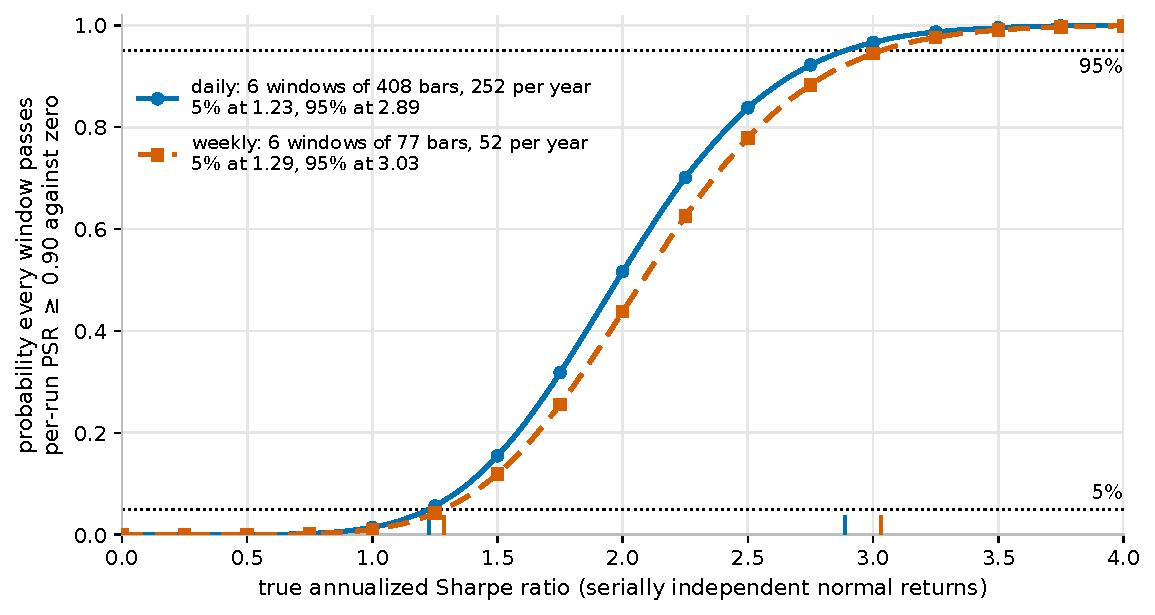
\includegraphics[width=\linewidth]{power-curve.pdf}
\caption{Probability that the default $\passk$ leg passes, every one of six windows reaching a per-run PSR of at least $0.90$ against zero, against the true annualized Sharpe of serially independent normal returns. Solid with circles: the daily geometry, six 408-bar windows at 252 periods per year. Dashed with squares: the weekly geometry, six 77-bar windows at 52 periods per year. Dotted lines mark 5 and 95 percent, and the short ticks above the axis mark where each curve crosses them. Monte Carlo over 200{,}000 replications per geometry; every point's standard error is at most $0.0012$, narrower than the line. A property of the gate under these assumptions, not a measurement of any agent. Drawn from \texttt{paper/evidence/final/power-curve.jsonl} by \texttt{python paper/src/make-power-curve.py figure}.}
\label{fig:power}
\end{figure}

\begin{table}[t]
\centering
\small
\caption{What each leg of the default gate requires, per default panel of \cref{tab:eligibility}. Bars is the window length and Bar (ann.) the panel's committed deflation benchmark. DSR min.\ is derived, not simulated: the smallest observed annualized Sharpe whose DSR against that bar, over the committed pooled length of six windows, reaches $0.95$ under normal moments (\cref{sec:power}). The four right-hand columns are Monte Carlo over 200{,}000 replications per window geometry with serially independent normal returns: the true annualized Sharpe at which the DSR leg, the $\passk$ leg, and both legs together pass with probability 95 percent, and at which both together pass with probability 5 percent. The bootstrap, process and mandate legs are not modelled and can only raise the full predicate's values above the both-legs columns. FX 1d and rates 1d share a window geometry and therefore a $\passk$ column. From \texttt{paper/evidence/final/power-curve.jsonl}.}
\label{tab:dsr-mde}
\setlength{\tabcolsep}{3.5pt}
\footnotesize
\begin{tabular}{lS[table-format=4.0]S[table-format=2.4]S[table-format=2.2]S[table-format=2.2]S[table-format=1.2]S[table-format=2.2]S[table-format=2.2]}
\toprule
 & & & & \multicolumn{4}{c}{True Sharpe (ann.) at pass probability} \\
\cmidrule(lr){5-8}
Dataset & {Bars} & {Bar (ann.)} & {DSR min.} & {DSR 95\%} & {$\passk$ 95\%} & {Both 5\%} & {Both 95\%} \\
\midrule
US indices 1w & 78 & 1.1382 & 1.69 & 2.25 & 3.01 & 1.35 & 3.01 \\
US indices 1d & 408 & 1.1382 & 1.67 & 2.20 & 2.89 & 1.32 & 2.89 \\
Crypto 1w & 46 & 1.1382 & 1.87 & 2.59 & 3.95 & 1.68 & 3.95 \\
Crypto 1d & 156 & 1.1382 & 2.17 & 3.20 & 5.64 & 2.38 & 5.64 \\
Crypto 4h & 990 & 1.1382 & 2.14 & 3.14 & 5.46 & 2.31 & 5.46 \\
Crypto 1h & 3990 & 27.3309 & 28.35 & 29.36 & 5.44 & 27.34 & 29.36 \\
FX 1d & 682 & 6.8254 & 7.25 & 7.68 & 2.23 & 6.83 & 7.68 \\
Commodities 1d & 677 & 1.1382 & 1.55 & 1.96 & 2.24 & 1.19 & 2.25 \\
Rates 1d & 682 & 3.4362 & 3.85 & 4.26 & 2.23 & 3.44 & 4.26 \\
\bottomrule
\end{tabular}
\end{table}


\subsection{What the evidence supports}\label{sec:claims}

Taken together, the findings support one claim and decline another. The claim has six parts, each scoped to the author-written field and the selected histories:
\begin{enumerate}[label=(\roman*),leftmargin=*,itemsep=2pt]
\item applied to reference agents on eight price-level datasets across four asset classes, plus one rates-yield stress series, at four bar sizes, the benchmark does not certify any of the unhedged long-only reference strategies as safe to hand capital under any of the three reliability verdicts (all-weather, never-catastrophic, or relative to same-window buy-and-hold), and it reports the drawdown that justifies the refusal;
\item the corrected luck floor never beats a reference agent, even when expanded to 1{,}000 agents on two daily datasets;
\item four rules whose specifications come from the published literature are refused in all 351 cells of \cref{sec:external}, including under a frictionless cost profile, so the refusal is not an artifact of the author's own strategy designs or of the cost calibration, although the implementations of those rules are ours;
\item all ten self-audit attacks are demoted by their commit-time tests;
\item the two committed golden fields reproduce byte-identically on Linux, macOS and Windows CI;
\item in a single common-random-number draw, a controlled injected edge is first admitted between annualized Sharpe $2.9$ and $4$, so the acceptance region is nonempty; where its boundary lies is not established beyond that draw.
\end{enumerate}
The eligibility conclusions are unchanged if the two realism-failing datasets are excluded: the verdict is zero eligible on all seven passing datasets as well, so nothing rests on the failed two. The refusal is a weak test of skill: under serially independent normal returns the all-weather gate on six windows passes an agent with a true annualized Sharpe of $1$ only $1.4$ percent of the time on the daily geometry and $1.1$ percent on the weekly, and reaches 95 percent only at $2.89$ and $3.03$ (\cref{sec:power}); on three panels the deflation gate cannot discriminate within the field (\cref{sec:passk}). The claim declined is that any external entity can attain eligibility, and that eligibility, where granted, means deployability. Eligibility certifies a statistically survivable edge under stylized execution on narrow universes, not capacity or breadth (\cref{sec:limitations}). Every completed entrant here is author-written, so the refusal is a finding about this field and these gates, not about the population of trading agents. The forward window \texttt{window-003} is open but unresolved, so a competing agent with genuine edge remains an outstanding experiment.

\section{Related work}\label{sec:related}

\paragraph{Skill and luck in finance.} The distinction the benchmark operationalizes is old. Applying a false-discovery correction to three decades of mutual funds, \citet{barras2010false} find that roughly three quarters had no genuine alpha and that most apparent winners were false positives; \citet{kosowski2006stars} reach a more nuanced verdict by bootstrap, and \citet{fama2010luck} the same conclusion by a different route. The Sharpe ratio itself is due to \citet{sharpe1966mutual}, and \citet{sharpe1994sharpe} restates it as a differential return over a benchmark; this paper uses the zero-rate raw-return form (\cref{sec:stats}). \citet{lo2002sharpe} works out the sampling distribution of the Sharpe ratio and shows its square-root-of-time scaling fails off IID returns, which bears on the annualization that this paper's first finding concerns. \citet{bailey2014pseudo} show that a high backtest Sharpe is trivially achievable by trying enough configurations, \citet{harvey2015backtesting} turn the observation into a haircut that scales with the number of strategies tried, and \citet{harvey2016cross} apply the same discipline to the factor literature. The probabilistic Sharpe ratio of \citet{bailey2012sharpe} and the deflated Sharpe ratio of \citet{bailey2014deflated} are the instruments this benchmark uses; the Reality Check of \citet{white2000reality}, the superior-predictive-ability test of \citet{hansen2005spa} and the step-down procedure of \citet{romano2005stepwise} are the field-wide tests it reports. \citet{arnott2019protocol} set out a protocol for backtesting in the era of machine learning, and \cref{sec:experiments} follows its multiple-testing and reporting items: every Sharpe is reported beside its number of trials, its track length, and the cost profile it was earned under.

\paragraph{Forward and adaptive evaluation.} Committing to an evaluation before the data exists is not new, and the benchmark's intended forward protocol is positioned against that lineage. The M competitions run genuine forward windows on data that does not exist at submission time; M6 in particular scored forecasting and investment performance jointly over a year of live monthly submissions \citep{makridakis2025m6}. On the adaptive-overfitting side, \citet{dwork2015holdout} give a mechanism that keeps a holdout valid under repeated adaptive queries, and \citet{blum2015ladder} bound leaderboard overfitting from adaptive resubmission; both attack the same disease as deflation by controlling the query channel instead of correcting the statistic. At least one live trading arena for LLM agents exists \citep{deepfund2025}. What the chained board adds is independently checkable byte history: scoring rules and entries are bound before operator-declared deadlines, and a re-signed forgery is exposed by the next window's anchor (\cref{sec:attest}). The hash chain does not prove the deadline's wall time, data custody or prior non-observation. SharpeBench has no completed forward result and no multi-window operating history: its two empty pre-entry records were superseded when the scoring-provenance requirements changed, and its first live window is open but unresolved.

\paragraph{Benchmarks for financial agents.} \Cref{tab:related} positions the benchmark against the boards it is most often compared with, on the axes the principles in \cref{sec:principles} make load-bearing. \Cref{tab:related-inverse} then draws the same comparison on the axes the rivals hold: every rival that fields agents scores real LLM or learned agents, most present a far richer information environment, StockBench runs single-name equities on a genuinely post-cutoff window with a live board, and the Open FinLLM Leaderboard is hosted under neutral governance. SharpeBench's row in that table is empty, its empty cells are the limitations of \cref{sec:limitations}, and the two tables together state the actual trade: statistical and adversarial properties, each an executed check rather than a guarantee, were bought at the price of field breadth, and the program of \cref{sec:limitations} is to pay that price back without giving up the guarantees. Each mark in both tables records what the cited paper or its public board states, not an inference; the per-cell sources, including the deliberate blanks, are committed beside the evidence (\texttt{paper/evidence/table-provenance.md}). The cells marked ? are the ones still unchecked: costs for FinBen and FinRL-Meta, and single names for FinBen and FinRL-Meta. A cell marked $\circ$ records a partial form of the property: two boards repeat their runs and report the mean or the median, which is not a requirement that every run pass. The comparison therefore supports the statement that none of these boards states both deflation and $\passk$, not that each lacks every property its row leaves blank.

Each rival's ranking metric explains one of the axes. FinBen \citep{finben2024} ranks GPT-4 first on its trading task and reports its Sharpe beside buy-and-hold's with overlapping marginal 95 percent confidence intervals across ten stocks (\cref{sec:intro}). Overlapping marginal intervals are not a paired test: a Welch test on the same summary figures gives $p$ between $0.026$ and $0.050$ depending on how the half-widths are read, so the published numbers are borderline evidence of a difference rather than evidence that none exists, and they carry no correction for search. StockBench \citep{stockbench2025} evaluates on a single four-month post-cutoff window and ranks on cumulative return, drawdown and Sortino, with no deflation. QuantBench \citep{quantbench2025} names overfitting as an open problem and ranks pipeline performance with no luck-corrected metric, though its simulation does charge commissions and transaction fees. InvestorBench \citep{investorbench2024} evaluates thirteen LLM backbones as decision-making agents across stocks, crypto and ETFs, and ranks on return-based metrics with no deflation or reliability gate. FinRL-Meta \citep{finrlmeta2022} is scoped differently: it supplies hundreds of gym-style market environments and data pipelines for training RL agents, a benchmark of environments rather than a gated board of submitted agents, so most gate axes do not apply to it; it is in the tables because any serious agent field would plausibly be trained in it. The FINOS Open Financial LLM Leaderboard \citep{openfinllm} measures financial knowledge, scored on accuracy and F1, and has no trading-performance axis. The reproducibility gap across this field is quantified by the evidence map cited in \cref{sec:intro} \citep{llmtradingaudit2026}.

\paragraph{Evaluation practice beyond the compared boards.} Recent trading and finance papers outside \cref{tab:related} show the same gaps, and several report them about their own work. On repeated runs, Backtrader-Bench reports that a single run without tools overstated one model's ten-run mean by more than 12 points, 76.7 against 64.3 percent \citep[p.~4]{zhao2026backtrader}. Agora reports its single-seed numbers ``for parity with the AlphaGen reporting convention'' and has run its full system at one seed \citep[pp.~15 and 33]{li2026agora}. A NeurIPS 2025 trading paper answers its checklist question on error bars with ``Our evaluation environment is deterministic'' \citep[p.~17]{ma2025robust}, while its agents are trained with PPO \citep[p.~39]{ma2025robust}; \cref{sec:principles} states what a deterministic scorer does and does not guarantee. On costs, BacktestBench sets transaction costs and taxes to zero in its baseline experiments \citep[p.~3]{wang2026backtestbench}, and StockBench states that it does not model trading costs, slippage or liquidity limits \citep[arXiv version 2, p.~9]{stockbench2025}. On search, Agora lists multiple-testing correction among the analyses it defers \citep[p.~34]{li2026agora}. On leakage, two systems report finding their own. In an earlier version of AQuA's loop, a reviewer agent approved a feature normalized by the whole day's volume, and a manual audit found the leak after the held-out information coefficient came out far above that of comparable features \citep[pp.~21--22]{guo2026aqua}; in another pipeline, an off-by-one date slice put validation-year returns into the training labels and inflated test Sharpe by 0.3 \citep[p.~11]{du2026multifactor}. \Citet[p.~7]{gencay2026survives} plants a look-ahead oracle that reaches a DSR of $1.00$, the case \cref{sec:integrity} addresses by enforcing the look-ahead boundary at the agent interface rather than through a statistic. On judges, FinTradeBench reports a mean absolute error of 0.40 on a 1 to 5 scale between its LLM judge and human expert scores, beside a Spearman correlation of 0.07 that it attributes to a ceiling effect \citep[p.~25]{agrawal2026fintradebench}, and CryptoAnalystBench reports quadratic-weighted kappa between 0.35 and 0.42 between its judge and domain experts \citep[p.~8]{eswaran2026cryptoanalyst}. SharpeBench has no judge, so this kind of agreement check does not apply to its scores.

Re-scoring a rival field is infrastructure here, not a result. An import adapter is contributed that converts a rival board's published per-period return series into scoreable submissions, embedding the caveat that imported fields carry no audit trace and unknown trial counts understate deflation, retaining each column's own observed date axis so that two series missing different dates are not paired by position, and refusing a period repeated within one run, which would otherwise enter the mean, the variance, the PSR sample length and the bootstrap twice. The keyed scoring path applies the same refusal to a field that did not come through the adapter. No rival re-scoring has been executed and no demotion of any rival's leader is claimed: StockBench publishes environment inputs and summary statistics but no per-agent return series, so the experiment awaits either the authors' raw artifacts or a reproduction with their harness, and until then the adapter is infrastructure, not evidence.

\begin{table}[t]
\centering
\footnotesize
\caption{Positioning along the axes this benchmark adds. A \checkmark{} means the cited source states the property; a $\circ$ means it states a partial form, here repeated runs reported as a mean or a median rather than required to pass on every run; an empty cell means a search found no positive evidence; a cell marked ? is unchecked, with no exhaustive search of the full text, and is not a verified absence. Per-cell sources are in \texttt{paper/evidence/table-provenance.md}, except three cells read from the full text on 17 September 2026 and not yet in that sheet: StockBench (arXiv version 2) runs each agent three times with different seeds and reports the average (p.~5), InvestorBench (arXiv version 1) reports the trajectory with the median metrics of five repeated epochs (p.~6), and the full text of that InvestorBench version states no transaction cost, commission, fee or slippage. $\tau$-bench, a customer-service agent benchmark, appears because it is the construct source for the seed leg of the reliability gate. Read together with \cref{tab:related-inverse}: a comparison drawn only on one's own axes is advertising.}
\label{tab:related}
\setlength{\tabcolsep}{4pt}
\begin{tabular}{lcccccc}
\toprule
 & Deflates & $\passk$ & Process gate & Costs & Deterministic & Forward commit \\
\midrule
FinBen \citep{finben2024} & & & & ? & & \\
StockBench \citep{stockbench2025} & & $\circ$ & & & & \\
QuantBench \citep{quantbench2025} & & & & \checkmark & & \\
InvestorBench \citep{investorbench2024} & & $\circ$ & & & & \\
FinRL-Meta \citep{finrlmeta2022} & & & & ? & & \\
Open FinLLM \citep{openfinllm} & & & & & & \\
$\tau$-bench \citep{taubench2025} & & \checkmark & & & & \\
SharpeBench (this paper) & \checkmark & \checkmark & \checkmark & \checkmark & \checkmark & \checkmark \\
\bottomrule
\end{tabular}
\end{table}

\begin{table}[t]
\centering
\footnotesize
\caption{The same comparison on the axes the rival benchmarks hold. A mark means the cited source states the property; an empty cell means the provenance sheet records no positive evidence after a search; a cell marked ? is recorded there as unchecked, with no exhaustive search of the full text, and is not a verified absence (per-cell sources in \texttt{paper/evidence/table-provenance.md}). FinRL-Meta's near-empty row reflects its different scope, an environment library rather than an agent board. SharpeBench's empty cells are its limitations (\cref{sec:limitations}), and three of them, the missing LLM field, the thin information environment, and the absent live board, are the price paid for the guarantees in \cref{tab:related}.}
\label{tab:related-inverse}
\setlength{\tabcolsep}{4.5pt}
\begin{tabular}{lccccc}
\toprule
 & LLM agents & Rich info & Single names & Live board & Post-cutoff run \\
\midrule
FinBen \citep{finben2024} & \checkmark & \checkmark & ? & & \\
StockBench \citep{stockbench2025} & \checkmark & \checkmark & \checkmark & \checkmark & \checkmark \\
QuantBench \citep{quantbench2025} & \checkmark & & & & \\
InvestorBench \citep{investorbench2024} & \checkmark & & \checkmark & & \\
FinRL-Meta \citep{finrlmeta2022} & & & ? & & \\
Open FinLLM \citep{openfinllm} & \checkmark & \checkmark & & \checkmark & \\
$\tau$-bench \citep{taubench2025} & \checkmark & & & & \\
SharpeBench (this paper) & & & & & \\
\bottomrule
\end{tabular}
\end{table}

\paragraph{Evaluation as a scientific object.} The reliability-versus-capability split that motivates the seed leg of $\passk$ originates in \citet{taubench2025}, which asks whether an agent succeeds on all $k$ attempts rather than on at least one. It is now a theme across agent evaluation: \citet{miller2024errorbars} argues for error bars on every evaluation score, \citet{kapoor2024agents} for cost-controlled evaluation and adequate holdout sets, and \citet{agentreliability2026} treats reliability as an axis separate from capability and finds that gains in the latter have not bought the former. The surveys that shape this paper's integrity section, \citet{betterbench2024} and \citet{constructvalidity2025}, find that most benchmarks neither report the statistical significance of their rankings nor allow their results to be replicated, and recommend an operational construct-validity checklist, which \cref{app:checklist} answers. A 2026 survey of financial multi-agent evaluation \citep{finmultiagentsurvey2026} catalogues five recurring failure modes: look-ahead, survivorship, backtest overfitting, transaction-cost neglect and regime-shift blindness. SharpeBench addresses look-ahead through point-in-time observations, selection through deflation, transaction costs through the simulator and regime dependence through $\passk$. It does not close survivorship in the fixed universes, which \cref{sec:limitations} states.

\section{Limitations}\label{sec:limitations}

We separate threats to external validity, which bound what the evidence can say about agents, markets and hosts beyond this study, from threats to internal validity, which bound whether the measurements are right on their own terms. The costliest admissions are in the first group. The history of repairs made after the evidence was frozen is recorded in \cref{app:repairs}, and capabilities that produce no result here are described in \cref{app:mechanism}.

\subsection{Threats to external validity}\label{sec:threats-external}

\paragraph{There is no external ceiling, and that is the paper's largest gap.} Benchmark papers that report a low score bracket it with an entity above the bar: OSWorld reports 12.24 percent for its best model against a 72.36 percent human ceiling \citep{osworld2024}, GAIA 15 percent for GPT-4 with plugins against 92 percent for human respondents \citep{gaia2024}, and SWE-bench 1.96 percent for its best model against a human-written patch that resolves every instance \citep{swebench2024}. SharpeBench has none. The synthetic witness of \cref{sec:witness} shows the acceptance region is nonempty on a sampled grid, in one draw, but we constructed the witness, so it bounds the predicate and does not measure any population. \Cref{sec:external} is the closest available substitute and it did not become a ceiling: four rules specified in the published literature, scored under three cost profiles, produce zero eligible cells and zero $\passk$ passes in 351 records, with the best of them at a deflated Sharpe of $0.6534$ frictionless against the $0.95$ bar. A reader therefore still cannot distinguish a well-calibrated gate from a miscalibrated one on external evidence alone.

Two things would supply a ceiling and neither is in reach here. The first is a real track record scored through the same gates: an audited fund or managed account's per-bar returns over six disjoint evaluation windows, which requires proprietary or permission-compatible data. The current frozen bundle does not meet that distribution condition (\cref{app:datasheet}). The second is a competing agent that clears the bar on the forward arena, which is what \texttt{window-003} is for and what no window has yet resolved. Until one of the two exists, every eligibility statement in this paper is a statement about the predicate and not about attainability by anyone.

\paragraph{The field is author-written, and no current-model result is admitted.} Every entrant in \cref{sec:experiments} was either written for this repository or implemented here from a published specification: reference agents, a risk-managed control, seeded random agents, a synthetic injected-edge family, and the four external rules of \cref{sec:external}. In the last case the specification is external and the implementation is ours, which removes the objection that the field encodes only its author's ideas and does not remove the objection that it encodes only its author's code. No third-party agent or third-party strategy implementation was scored, so the headline refusal is a finding about an author-written field, not about the systems the benchmark is built to evaluate. A model-agent path is implemented: SharpeArena \citep{toca2026sharpearena} runs the point-in-time environment and canonical fail-closed parser, writes a complete append-only field journal, and compiles it across an artifact boundary into the submissions SharpeBench evaluates. Its scheduler, sharding, resume, provenance and fault semantics are tested with deterministic doubles. None of that is an agent result. Every empirical claim in this paper therefore remains about the protocol's behavior on entrants whose properties are known by construction.

\paragraph{The window rule refuses whole strategy classes by design, not by the gates.} The observation carries twenty trailing closes and each run starts fresh at its window boundary, so a rule needing $L$ closes is blind for the first $L-20$ bars of every window (\cref{sec:external}). The canonical trend rules of the published literature are stated over ten to twelve months, and at the shipped window rule \texttt{faber-10m} cannot form its signal on any bar of the six windows on daily crypto, 4-hour crypto or hourly crypto, and is blind for 190 of every 408-bar daily US window. Any entrant whose edge lives at that horizon is therefore refused by the experiment design and not by the gates, which makes the six-window rule a load-bearing choice this paper has not ablated. Lengthening the windows trades that away against the number of evaluation windows, and so of regimes, the reliability leg can test, and the trade is not evaluated here.

\paragraph{The operator is host, key holder, potential competitor and adjudicator.} Intake, epoch advancement, held-out-data custody, sealed scoring, signing and publication are operator-driven (\cref{sec:attest}); the policy permits the host to compete on a future board; and a disputed entry is adjudicated by the operator, with no third-party arbiter, neutral host or key escrow (\cref{sec:governance}). A signed chain proves that a published history was not altered. It does not prove that the operator was disinterested when producing it, and nothing in the artifact can.

\paragraph{The refusal has low statistical power.} At the shipped geometry of six windows and a per-run PSR bar of $0.90$ against zero, and under serially independent normal returns with the same edge in every window, the all-weather gate passes an agent with a true annualized Sharpe of $1$ only $1.4$ percent of the time on the daily geometry and $1.1$ percent on the weekly, passes one of $2$ about half the time, and reaches 95 percent only at $2.89$ and $3.03$; on daily and 4-hour crypto, whose windows span under half a year, reliable admission by both modelled legs needs $5.64$ and $5.46$ (\cref{sec:power}). On hourly crypto, daily FX and daily rates the measured deflation bar is high enough that every agent scores a deflated Sharpe of exactly zero at the default configuration, so on those panels the deflation gate does not discriminate within the field; the minimum observed annualized Sharpe the DSR leg can admit there is $28.35$, $7.25$ and $3.85$ (\cref{tab:dsr-mde}). Real returns are not independent normal draws, so these probabilities describe the gates, not any agent. Universal refusal is what this design predicts for a field with no skill and also for a field with realistic skill, so the refusal is evidence of strictness, not evidence of absent skill.

\paragraph{The scoring grid is wide along the leg that does not bind.} The 64 host configurations behind the 4{,}608 records vary $\beta$, the observable trial count and the dispersion source, and across all 64 only the deflated Sharpe moves: in every one of the 72 verdicts the $\passk$ result, the bootstrap $p$-value, the process result, the PSR and the worst-run drawdown are identical (\cref{sec:passk}). On the six panels whose bar is the precommitted floor, that is the leg that does not decide the conjunction: $\passk$ sets the 95 percent point there to within $0.01$ (\cref{sec:power}), and $\passk$ binds on both witness geometries under the exogenously calibrated bar (\cref{sec:witness}). Only on hourly crypto, daily FX and daily rates does the measured deflation bar set it. Meanwhile the two parameters that decide $\passk$ are fixed throughout this paper: the per-run PSR bar at $0.90$ (\cref{sec:predicate}) and the number of evaluation windows at six. Neither is ablated. A per-run PSR bar axis over, say, $\{0.50, 0.75, 0.90, 0.95\}$ would answer the question the grid does not, whether the universal refusal survives a weaker per-run requirement or is manufactured by a strict one, and that answer would change how \cref{tab:eligibility} should be read more than the other 63 configurations do. It is absent because the frozen records carry per-agent summaries and no per-run return streams, so the axis is a re-score of the whole field rather than a re-read of the evidence, and this revision regenerates nothing (\cref{app:repairs}).

\paragraph{The false-positive rate is not measured.} The only Type-I statement in this paper is analytic: at a true Sharpe of zero no replication passed on either geometry (\cref{sec:power}), computed under serially independent normal returns, which is the assumption \cref{sec:stats} says these panels do not satisfy. Its empirical counterpart, the 1{,}000-agent luck floor of \cref{sec:luck1000}, was run under the typical cost profile alone, where every zero-skill track already has a negative raw mean return before a gate sees it; that floor therefore measures the cost model together with the gates and cannot separate them. The measurement that would separate them is identified and cheap: rerun the same floor frictionless on \texttt{us-indices-1d} and \texttt{crypto-majors-1d} and report the share of the 2{,}000 zero-skill agent-dataset cells that clears the full predicate. That share is a false-positive rate on real fat-tailed, volatility-clustered returns with the cost drag removed, which is the condition under which the floor tests the gates rather than the costs. The producer already accepts the frictionless profile, and the three-profile external sweep of \cref{sec:external} completes in 129.3 seconds, so a profile flag and a rerun are what stand between this paper and the number. It has not been run. SharpeBench therefore ships with no measured false-positive rate, and nothing here should be read as one.

\paragraph{Coverage and observation.} Single-name equities are absent for want of a keyless feed, gold because the public daily series were withdrawn, and two of nine datasets fail the realism battery and ship with the verdict recorded. The crypto and index symbol sets were selected with hindsight from assets that survived into the collection period; the fixed universes therefore do not close survivorship bias. The nine dataset-timeframe combinations reduce to roughly five independent market panels, all containing at least one labeled bear window; only the longer panels contain both the 2020 and 2022 drawdowns. The refusals of \cref{sec:passk} are properties of the gates on these selected histories rather than of the gates alone. Apart from crypto spot, the series are price levels rather than tradable total-return positions: equity indices without dividends, spot FX without carry and spot oil without roll yield (\cref{sec:stats}). The rates file contains the 10-year constant-maturity yield itself, not a tradable Treasury price or total-return index; treating its percentage level as a price makes that row a simulator diagnostic rather than evidence about a bond strategy, and none of the eligibility conclusions depends on retaining it. Capacity and volume-based market impact are not modelled (\cref{sec:simdata}). The agent sees twenty trailing closes; the protocol carries fields for fundamentals and news and the simulator leaves them empty, so this is a thinner information environment than FinBen or StockBench present.

\paragraph{The reliability gate is strict by construction.} The default certifies profitability in every regime, and \cref{sec:passk,sec:ablation} show that both it and a per-run drawdown bound refuse every long-only reference agent on every dataset containing a downturn; \cref{sec:relative} reaches the same verdict under the benchmark-relative question. Which of the three is the right definition of safe for a given mandate is the operator's choice, now exposed as configuration, and \cref{sec:predicate} states why the conservative default ships anyway; the paper does not claim to have found the right default. A typed mandate declared at submission is built (\cref{sec:mandate}), but a relative declaration cannot be definitively verified from a lone trajectory: the verifier fails closed with an explicit aligned-field-benchmark requirement. On short windows the per-run PSR bar is weak because the statistic scales with $\sqrt{n-1}$, which is a property of the PSR and not a choice. Eligibility, where it is ever granted, certifies a statistically survivable edge under stylized execution on narrow universes; it is not a deployability, capacity, or breadth certificate.

\paragraph{Named experiments still open.} No current-model field has completed or produced an admitted performance artifact. The implemented path records model, runtime, scaffold, decoding, cadence and fault metadata, but those are protocol capabilities rather than results. A future field must predeclare its target population and treat materially different inference configurations as separate arms. The synthetic witness has not been replicated over independent noise draws (\cref{sec:witness}). The forward arena has one open window, \texttt{window-003}, bound to the attested v0.9.0 release binary; it carries no commitment yet and, at the manuscript cut, has not reached its declared resolution epoch, so no forward result is reported here (\cref{sec:attest}). Until neutral hosting and key custody exist the board remains a single-author artifact. The StockBench reproduction through the import adapter still awaits per-agent return series (\cref{sec:related}). No human, practitioner or recognition validation study has been run (\cref{sec:principles}).

\subsection{Threats to internal validity}\label{sec:threats-internal}

\paragraph{The statistics carry assumptions the data do not meet.} A September 2026 audit read the kernel against its primary sources and changed claims, not numbers. The default dispersion prior is a free choice and not the cited worked example, which implies a standard deviation $\sqrt{2}$ larger (\cref{sec:units}). PSR and DSR assume serially independent returns, which neither the frozen datasets nor the synthetic generator satisfy; only the bootstrap $p$-value and interval account for serial correlation, and the autocorrelation-adjusted variance of \citet{lopezdeprado2026howto} is available only as an opt-in diagnostic the gate does not read (\cref{sec:stats}). PSR is one minus a $p$-value, not a probability that the true Sharpe exceeds its benchmark. The Sharpe ratio uses a zero risk-free rate on price-level inputs, which is conservative for the refusals with respect to the cash rate and of undetermined direction with respect to dividends, carry and roll (\cref{sec:stats}). The tail-seller self-audit case exercises an event only the audit produces, and imported return series have no protection against option-like payoffs (\cref{sec:selfaudit}). A regression test now pins the deflated Sharpe worked example to its printed values (\cref{app:commands}).

\paragraph{The tables come from an older engine and carry no interval.} Every table and figure in \cref{sec:experiments} except the synthetic witness was produced by the v0.9.0 snapshot and was not rescored after the repairs of \cref{app:repairs}, which change what the current engine would compute: corrected standardized-moment estimators, a simulator repair, a reference-agent repair, a reconstruction difference on commodities, and the refusal of a constant track such as \texttt{hold}'s (\cref{sec:predicate}). The size of the resulting shifts in the tables is not established; where this paper says a repair left eligibility and ordering unchanged, the statement covers only the two deterministic score fixtures that were actually refreshed. The frozen records also carry no DSR interval, so the tables print point estimates without the resolution band that would say which differences are real (\cref{sec:passk}).

\paragraph{Honor-system inputs and field-level gaming.} Declared trial counts remain unverifiable for arbitrary submissions. The generated-strategy path closes only the part it observes: every raw candidate produced inside that harness is counted before validation or deduplication and the selected candidate alone reaches a disjoint test interval. It cannot count private or pretraining search, so \cref{sec:incentives} keeps declared-$N$ advisory outside that path. The measured dispersion is set by whoever populates the field, and its near-clone Sybil vector is now closed: ranking collapses clone clusters to one vote before measuring, and the ninth audit case asserts on every commit that 200 sock puppets no longer move the bar (\cref{sec:sybil}). The configured dispersion floor bounds, rather than closes, the adversary who submits genuinely dissimilar low-dispersion streams: such a field can still relax an honest measured dispersion down to the precommitted prior, roughly a tenfold reduction on the audit's fixture, and the guarantee is only that it stops there. Nothing bounds the measured dispersion from above, so a submitter can still raise every rival's bar with deliberately poor but scorable agents; the degenerate version, an entrant whose track has no Sharpe ratio at all, no longer votes (\cref{sec:incentives}). Clone collapse also interacts with seed averaging, and on five of the nine panels it merges honest agents and forces the configured fallback (\cref{sec:sybil}). The bootstrap gate is not corrected for the number of agents tested (\cref{sec:predicate}). Distinct verified identities and per-identity entry caps remain unbuilt. Backtest verdicts for pretrained models are advisory by protocol rule because contamination, not multiple testing, is the binding threat there (\cref{sec:incentives}); the shape-level contamination probe that would test this, scoring the same agent on real and moment-matched surrogate series, is specified but not run.

\paragraph{The forecast report has no empirical field here.} The deterministic cross-product tutorial in \cref{sec:forecast-quality} proves file compatibility and exercises the scorer, not forecast skill. A superseded convenience-sample lifecycle pilot remains archived so that its protocol history is not rewritten, but its obsolete checkpoint scores are excluded from the paper, model comparison and trading rank. Even a future field inherits four limits. Exact pair support stops an agent from choosing its own comparison set, but a field of partial documents may leave many pairs without inference, a withheld pair says nothing about which agent forecasts better, and the contracts two agents share may be few or unrepresentative; resolution-time blocks encode a declared dependence unit and do not prove longer dependence absent; the current analyzer pools contracts of different scoring rules into one pairwise difference, which is valid only within a single stratum; and proper forecast scores measure predictive distributions, not execution quality, transaction costs, risk controls or portfolio value. Those are the reasons the report cannot enter \cref{eq:eligible}.

\paragraph{Built and not yet exercised.} The arena lifecycle is built and one window, \texttt{window-003}, is open, but it holds no commitment and no completed board exists. A daily workflow advances deadline states, and there is no hosted intake and no live board UI; scoring, signing and publication remain operator-driven, so the league is not yet a running service and the governance policy of \cref{sec:governance} is a policy the operator applies rather than one a third party can enforce. External agents are sandboxed by container isolation only, which is the subject of the paragraph below; multi-tenant hosting of untrusted submissions remains unbuilt. No completed real entrant triggers the process gate in the evidence field: that gate is exercised by synthetic demonstrations and all nine of the kernel's adversarial audit cases, so its enforcement is tested but its field prevalence is unknown. The perturbation diagnostic of \cref{sec:perturb} narrows the self-audit's blind spot but samples perturbations rather than searching adversarially, so a fragility that survives sampling can still hide. The calibration module splits uncertainty into aleatoric, epistemic and distributional legs after the taxonomy of \citet[p.~2]{lin2025trading}, with estimators re-derived for a kernel that has no model. Its epistemic leg reads agreement among an agent's confidence streams as low uncertainty, so unanimous-but-wrong signals read as agreement and the leg is informative only when it reads high. Every experiment other than \cref{sec:external,sec:seedleg} uses the typical cost profile. \Cref{tab:costsens} reports all three shipped backtest profiles, and it bounds the cost objection without removing it: no cell is eligible under any profile, so the universal refusal is not produced by the cost calibration, but the profile does move the deflation bar itself, from $1.2576$ frictionless to $27.5397$ typical on hourly crypto, because the measured field dispersion widens as the cost drag on zero-skill agents grows. The frictionless column is also not a clean counterfactual: it removes fees, slippage, rebalancing cost and financing at once, and the stressed column does not apply \texttt{CostProfile::WorstCase}'s two-bar decision delay, because the backtest driver consumes the cost model only. The falsification leg still inherits the narrower version of this limitation: every zero-skill track in the 1{,}000-agent floor has a negative raw mean return under the typical profile, so the floor demonstrates that costs plus deflation keep noise below the bar, and the cost-free lucky tail was not rerun at 1{,}000 agents.

\paragraph{The live sandbox boundary is exercised in one Docker configuration.} Everything the container sandbox decides before launch is a pure function and is tested without Docker. The boundary itself is not: the \texttt{sandbox} continuous-integration job pulls \texttt{alpine:3.22}, resolves it to an immutable digest, refuses a mutable fixture and runs the ignored live tests on a Docker-enabled Linux runner. The in-container readiness probe checks a non-root user, zero Linux capabilities, no-new-privileges, loopback-only network visibility, a read-only root, a bounded writable temporary filesystem and a \texttt{noexec} temporary mount. Separate probes attempt egress to cloud metadata, the wider link-local range, all three RFC1918 blocks, the public internet and a live listener on the host loopback; each must be classified as a policy denial within the configured time bound, rather than merely failing after a timeout. A production-spawn smoke test verifies that the fixture actually starts, and a 32~MiB live cgroup test must end in a memory-breach verdict, which the harness maps to a non-retryable agent resource fault before removing the named container. Docker records an out-of-memory kill through an asynchronous flag that can be lost, so the verdict also reads the exit status a kernel kill leaves. The same job launches the model gateway against the fixture with no network, runs the image preflight and its runtime allowlist against it, and captures and re-executes a trajectory through the hardened launch.

These observations establish less than a general containment proof. They cover one hosted-runner and daemon configuration, one benign POSIX fixture and the named probes; no hostile trading entrant or multi-tenant service has been evaluated, and they do not rule out a Docker or kernel escape. Ordinary suites report the live-boundary tests as ignored unless their Docker prerequisites are explicitly enabled; only the dedicated job counts them as evidence. That distinction is deliberate: an earlier runtime skip and a weak ``no orders'' assertion could both pass when the container never started. The current tests require a live prerequisite, a specific denial class or an observable Docker state, so missing infrastructure cannot masquerade as evidence. A harness terminated by uncatchable \texttt{SIGKILL} between spawn and cleanup can leave a stopped, inspectable named container; normal completion and object destruction both remove it, but the implementation does not claim leak-freedom against termination that prevents either path.

\paragraph{Protocol corrections and their scope.} The paper records four limitations of earlier protocol configurations: a deflation prior in the wrong units (\cref{sec:units}); an incorrect documentation claim that field-wide significance tests gated rank (\cref{sec:stats}); a private HMAC chain described as publicly verifiable (\cref{sec:attest}); and a one-symbol luck floor that degenerated into a buy-and-hold clone, whose degeneracy produced a spurious rates-panel DSR of $0.993$ that the corrected construction removes (\cref{sec:falsify}). The current protocol and evidence address these specific defects. They do not turn a reference-agent study into evidence of deployability, field breadth or a live league. A fifth change belongs beside them without belonging to the list, because it is not a correction: closing the agent wire contract in v0.11.0 broke entrants written against v0.10.x, shipped with no deprecation window, and was recorded in the v0.11.0 changelog entry under a fixes heading that understated it (\cref{sec:benchmark,sec:governance}). It is released and cannot be unshipped, and the migration is to drop the offending key or move it into one of the two fields that accept free content.

\section{Reproducibility statement}\label{sec:repro}

The benchmark is twelve library crates under \texttt{crates/}, plus a thirteenth Python-binding crate excluded from the Rust workspace because it is built by maturin; the workspace itself lists fourteen members, the twelve libraries plus \texttt{xtask} and the reference-agent example. It is licensed MIT and Apache-2.0 and published to crates.io, npm and PyPI, with a pinned toolchain and a lockfile. The artifacts in this paper are the v0.9.0 tag stated in \cref{app:commands}; later releases do not change them, and the registries serve the latest tag rather than that one. The scoring kernel forbids unsafe code. Every dataset in \cref{tab:data} is committed with a SHA-256 sidecar and a fetch script whose check mode reproduces the committed bytes from the public source. Every figure in this paper is produced by a committed script from the kernel's own formulas, and every table is produced by the commands in \cref{app:commands} from the committed data. Golden fixtures pin the full ranked output of two fields at full floating-point precision and are checked on Linux, macOS and Windows on every commit; a parity test asserts that WebAssembly and native scores are byte-identical. The self-audit runs on every commit: the build fails if any of the nine claimed defenses regresses, and the Sybil case additionally fails if the attack stops reproducing with the clone collapse switched off, so the defense cannot be counted as a pass by the attack quietly ceasing to work. Continuous integration for the commit this paper was built from is green on every job: the eight defined in the main workflow (\texttt{check}, \texttt{test}, \texttt{python}, \texttt{determinism}, \texttt{audit}, \texttt{realism}, \texttt{supply-chain} and \texttt{docs}), two of which, \texttt{test} and \texttt{determinism}, fan out across Linux, macOS and Windows, plus the npm and forward-arena workflows.

No large language model is a component of the benchmark or of any result in this paper; the kernel has no judge. Language models were used to draft and edit prose; no citation in the bibliography was generated by one, and every arXiv entry was checked against its abstract page.

\section{Ethics and broader impact}\label{sec:ethics}

A benchmark that certifies trading agents has a shorter path to harm than a benchmark that certifies code edits. An eligibility verdict is a fitness claim about software that moves money, and a badge is the artifact a retail marketer would reach for first. This section states what the verdict does and does not assert, the conflicts the artifact carries, and why it is released anyway.

\paragraph{What eligibility is not.} Eligibility certifies that an entrant's edge survived five statistical and process tests on frozen historical bars under a stylized execution model. It is not investment advice, not a prediction of live performance, not a capacity, breadth or liquidity certificate, and not a statement about any instrument. It is conditional on the configuration digest, the field the entrant was scored against and the histories in the window: \cref{sec:passk,sec:external} show the same agent's deflated Sharpe moving when the field composition changes and when the cost profile changes, so a verdict quoted without its configuration is not a verdict. The board prints the refusing gate and the quantity that produced it, which is the only form in which we intend a score to be quoted.

\paragraph{Dual use.} The same properties that make the protocol hard to game make it attractive to cite selectively. An entrant that clears the gate on one dataset can advertise the pass and omit the eight refusals; an operator can lower \texttt{dsr\_bar} or the per-run bar and publish the resulting admissions under the SharpeBench name. Two mechanisms bound this and neither closes it. The scoring configuration is serialized and digest-committed on every board, so a relaxed bar is visible to anyone who verifies the board, and the signed chain of \cref{sec:attest} makes a board that omits its own configuration unverifiable. What we cannot prevent is a screenshot. The countervailing consideration is that the failure mode this work exists to correct, a leaderboard that ranks the best overfitter and calls it the best agent, is already in circulation, and an artifact that refuses is a weaker marketing instrument than one that ranks.

\paragraph{Asymmetry of errors.} The gate is calibrated to under-certify. A false positive hands capital to a strategy whose edge was noise; a false negative costs an entrant a badge. We chose the direction deliberately, and the cost of that choice falls on entrants rather than on the public. It is still a cost: \cref{sec:external} shows four published rules and a risk-managed control refused on every panel, and a strict gate that refuses everything is not automatically a correct gate. The synthetic witness of \cref{sec:witness} is what stops that argument from being unfalsifiable, and it is the only demonstration in this paper that anything can pass.

\paragraph{Conflict of interest.} The policy permits the host to compete on a future board, but no model-entry board has been published. Every offline entrant reported here is either written for this repository or implemented here from a published specification, the operator holds the Ed25519 signing key, and intake, sealed scoring, signing and publication are all operator-driven (\cref{sec:attest,sec:governance}). The chain proves that a published history was not altered; it does not prove that the host was disinterested when it produced that history. Neutral hosting, third-party key custody and an external dispute procedure are named in \cref{sec:governance} as unbuilt.

\paragraph{Data and licensing.} All nine datasets were collected without API keys, but keyless access did not establish redistribution permission. The three US index series are copyrighted and marked pre-approval required; no approval is recorded. FRED's federal-source series carry its \enquote{Public Domain: Citation Requested} category but remain subject to the service-wide prohibited uses, and the reviewed Binance pages grant access without granting this repository redistribution rights. The code is MIT or Apache-2.0; that license does not extend to the observations. This is an unresolved data-distribution blocker, not a claim that the historical evidence used different bytes. \Cref{app:datasheet} gives the series-level record and remediation choices.

\paragraph{Market effects.} The benchmark does not trade. It replays frozen historical bars through a simulator, so scoring an agent has no market impact and consumes no venue capacity. The forward arena of \cref{sec:attest} scores on data that postdates the commitment, and it likewise scores rather than executes: no window has ever placed an order.

\paragraph{Release calculus.} The tension is that publishing a certification protocol for capital-allocating agents makes certification easier to claim as well as easier to check. We release because the checking half is verifiable by anyone and the claiming half is not: every number here recomputes from committed data by a listed command, the nine self-audit attacks run on every commit, and a reader who doubts a verdict can regenerate it. A protocol that only its author can execute would carry the same dual-use exposure and none of the accountability.


\bibliographystyle{plainnat}
\bibliography{refs}

\appendix
\section{Commands that produce every number}\label{app:commands}

All commands run from the repository root at the tagged version. The kernel is deterministic, so each command produces the same bytes on any platform.

\paragraph{Version.} Findings 1 and 2 were first observed at v0.2.1. The units fix is v0.3.0. The configurable reliability gate, the per-run drawdown bound, and the evidence sweep that scores both verdicts on identical trajectories are in the release after it. \Cref{tab:units} was computed against v0.2.1; every other table and figure against the later kernel.

\paragraph{The shipped demonstration (\cref{fig:demotion}).}
\begin{verbatim}
sharpebench score suites/example_submissions.json
\end{verbatim}

\paragraph{The deflation curve (\cref{fig:deflation}) and the demotion chart.}
\begin{verbatim}
python paper/src/make-figures.py
\end{verbatim}
The script reimplements the kernel's PSR, expected-maximum-Sharpe and normal-quantile functions in Python and states that it does; the figures are the kernel's formulas, not an independent computation.

\paragraph{The self-audit (\cref{tab:attacks}).}
\begin{verbatim}
sharpebench audit
\end{verbatim}

\paragraph{Data realism (\cref{tab:data}).}
\begin{verbatim}
sharpebench realism --data data/<dataset>.csv
\end{verbatim}

\paragraph{Regenerating any dataset and checking its hash.}
\begin{verbatim}
python scripts/data/fetch_crypto.py --interval 1h --check
python scripts/data/fetch_fred.py fx --check
python scripts/data/derive_weekly.py --check
\end{verbatim}

\paragraph{The evidence sweep (\cref{tab:eligibility}, \cref{sec:units}, \cref{sec:passk}, \cref{sec:ablation}, \cref{sec:falsify}).}
\begin{verbatim}
cargo run --release -p sharpebench-harness \
  --example evidence_sweep -- out.jsonl [dataset] [dsr_bar]
\end{verbatim}
One JSON record per (dataset, configuration, agent), 512 per dataset. The grid, seeds, window rule, cost profile and both reliability configurations are constants in the source and are emitted on every record. The optional arguments restrict a run to one dataset or one deflation bar so the grid can be split across processes; because every seed is pinned, the concatenation of parts is identical to a serial run. The analysis that turns the records into the tables is a short script committed beside them under \texttt{paper/evidence/}.

\paragraph{Golden fixtures and the parity test.}
\begin{verbatim}
cargo test -p sharpebench-core --test golden_scores
cargo test -p sharpebench-sim  --test golden_input
cargo test -p sharpebench-wasm --test native_parity
\end{verbatim}
Regeneration requires \texttt{SHARPEBENCH\_UPDATE\_GOLDEN=1} and refuses to run when \texttt{CI} is set.

\paragraph{Signing and verifying a board.}
\begin{verbatim}
sharpebench sign   subs.json <hmac-key> board.json --ed25519 <secret>
sharpebench verify board.json --public
sharpebench verify board.json --pubkey <hex>
\end{verbatim}
The second form verifies from the document alone. The third pins the key and rejects a board re-signed under a different one.

\section{Construct validity checklist}\label{app:checklist}

\citet{constructvalidity2025} review 445 benchmarks and recommend that a benchmark paper answer an operational checklist. Each answer points to the section that supports it.

\begin{description}[leftmargin=*,itemsep=3pt]
\item[Define the phenomenon.] Yes. The phenomenon is skill that survives five eligibility conjuncts: deflation for the number of trials, $\text{pass}^{k}$ across seeds and windows, process discipline, a bootstrap null and the configured mandate. \Cref{sec:principles} states it and \cref{eq:eligible} operationalizes it exactly.
\item[Measure only the phenomenon.] Partly. The eligibility predicate measures the phenomenon and nothing else. The scorer also reports fourteen statistics that do not gate, and \cref{sec:predicate} separates the two so a reader can tell which number moved the rank.
\item[Construct representative datasets.] Partly. Eight tradable-price datasets across four asset classes, plus one rates-yield stress series, use four bar sizes and are scored for realism before use (\cref{sec:data}), with provenance in \cref{app:datasheet}. The coverage gaps, unresolved distribution rights, two realism failures and twenty-close observation are stated in \cref{sec:limitations}.
\item[Acknowledge limitations of reused datasets.] Yes. Every dataset's source, license, caveats and failing stylized facts are in \cref{tab:data} and the data scripts. The commodities file keeps a negative oil close as published and documents the opt-out.
\item[Prepare for contamination.] Yes, at the mechanism level. Sealed held-out datasets under a published hash, a canary token, and a masked view that defeats ticker memorization (\cref{sec:contamination}). A forward commitment binds artifact bytes before an operator-declared deadline, while wall time, custody and prior non-observation remain trust assumptions (\cref{sec:attest}). The forward league that would exercise it has not run.
\item[Use statistical methods.] Yes. Every rank is gated on a deflated Sharpe with its number of trials, a block bootstrap with a fixed seed, and a per-run reliability test; field-wide Reality Check, SPA and step-down are reported; a bootstrap confidence interval on the DSR marks tied entries as tied. The annualization convention is stated once in \cref{sec:stats} because getting it wrong was the first finding.
\item[Conduct error analysis.] Yes. \Cref{sec:experiments} traces every refusal to the gate that produced it and the quantity that justified it, and one of the four numbered findings began as an error in the benchmark itself, with three further defects recorded in \cref{sec:limitations}.
\item[Justify construct validity.] Partly, and the gap is named. The benchmark refuses every reference agent for reasons the data makes explicit, the luck floor never beats a reference agent, and the synthetic witness of \cref{sec:witness} shows the acceptance region is nonempty and locates its boundary. What it has not shown is a real agent being admitted, so the claim that a real strategy can attain eligibility awaits the competing agent listed first in \cref{sec:limitations}.
\end{description}

\paragraph{Statistical reporting.} Every Sharpe in this paper is per period unless stated annualized, and \cref{tab:units} gives the conversion at every bar size. Every deflated Sharpe is reported beside its $N$. All runs use eight execution seeds and six windows; the per-cell record carries both. Costs are the typical profile of \cref{app:simdata}. Block bootstrap, not i.i.d., throughout.

\paragraph{Licenses and maintenance.} Both are in \cref{app:datasheet}, under Distribution and Maintenance. In summary: the code is MIT or Apache-2.0, but that license does not cover the observations. The three US index series require pre-approval, no Binance redistribution grant is recorded, and the current FRED service terms constrain the other series' use. This remains a distribution blocker. Historical dataset identities are frozen by hash and retired rather than edited; a permission-compatible replacement requires new identities and a new empirical run. Golden fixtures change only by a local command that refuses to run in continuous integration.

\paragraph{Compute.} Hardware, wall clock, peak memory and the zero-API-cost claim are reported in \cref{sec:experiments}: the full 4{,}608-cell grid regenerates in 2{,}078 seconds on one core, with no network, no key and no GPU.

\paragraph{Ethics.} \Cref{sec:ethics} states what an eligibility verdict does and does not assert, the dual-use exposure, the host's conflict of interest, and the release calculus. \Cref{sec:governance} states who may enter, that a published score cannot be retracted, the per-window variant cap, how a scoring defect is handled after publication, and that dispute adjudication is currently the operator's.

\section{Simulator, data, replay and contamination}\label{app:simdata}

\subsection{Simulator and cost model}

The data store returns rows at or before the decision index. The agent observes the close at bar $t$ and its order fills at that same close, with costs applied to the fill price. That close-to-close convention is idealized; the direction and size of a decision delay's effect on each entrant are not established, and a delay sensitivity is planned. Execution charges a per-trade fee, seeded slippage, a size-dependent rebalancing cost that scales with the square root of the trade's value as a fraction of the agent's own net asset value, and financing on gross exposure above one times net asset value. A per-step turnover cap can limit each trade to a fixed fraction of net asset value. Both the rebalancing cost and the cap are measured against the agent's book: the datasets carry no volume, so neither is a share of market volume, capacity and volume-based market impact are not modelled, and a small book and a large one pay the same rate. Four named cost profiles ship, and each is reported under the name used throughout this paper rather than under its Rust identifier: frictionless (\texttt{CostProfile::None}), typical (\texttt{CostProfile::Typical}), stressed (\texttt{CostProfile::WorstCase}) and realistic (\texttt{CostProfile::Realistic}). The typical profile is 2 basis points fee, 3 slippage, 50 rebalancing cost and 5 financing; stressed is 10, 15, 150 and 20 with a per-step turnover cap of 10 percent of net asset value and a two-bar delay, which the backtest driver does not apply; frictionless charges none of them. Realistic is typical plus seeded fill delay, partial fills and queue-position slippage. \Cref{sec:external} sweeps frictionless, typical and stressed; \cref{sec:seedleg} compares typical with realistic on three daily datasets; every other experiment uses the typical profile. The seeded slippage is what makes different execution seeds produce different runs and gives $\passk$ something to measure.

\subsection{Data}\label{sec:data}

Nine frozen datasets supplied the historical benchmark evidence, each with a SHA-256 sidecar and a deterministic fetch or derivation script. The source requests needed no API key, but that access fact did not grant redistribution permission; \cref{app:datasheet} records the unresolved rights blocker. \Cref{tab:data} lists the exact historical bytes and date ranges. Before any agent is scored on a dataset, the dataset is scored: a battery of stylized facts after \citet{cont2001empirical} tests excess kurtosis, volatility clustering, gain-loss asymmetry and aggregational Gaussianity, and time-reversal asymmetry after \citet{zumbach2009time}, and issues a verdict. Seven of the nine pass. Weekly US indices fail the aggregation test because 522 bars is too short for it, and FX majors fail the time-reversal asymmetry test, which does not detect the asymmetry at its threshold on these daily noon buying-rate series. Both ship with the verdict recorded. Apart from crypto spot, every series is a price level rather than a tradable total-return position: the equity series are price indices without dividends, the FX series are spot rates without carry and the oil series are spot prices without roll yield (\cref{sec:stats}).

Two datasets carry caveats the scripts document. The commodities file keeps the WTI close of $-36.98$ on 20 April 2020 as published, which dominates its moments, so every commodities statistic in the paper inherits that outlier; a start date of May 2020 is the documented opt-out and removes it. The rates file's close column is a yield in percent, not a price. The simulator nevertheless treats that column as a price level, so its percentage changes are neither Treasury total returns nor the P\&L of a duration-specified bond position. That row is a numerical stress case for the protocol on a one-symbol universe and must not support an economic performance claim: cross-sectional momentum is undefined there, and the luck floor requires the single-symbol randomization of \cref{sec:falsify} to be a control at all. \Cref{sec:limitations} states the coverage gaps.

\subsection{Replay and recompute}\label{sec:replay}

A captured trajectory contains the agent's raw decisions and a schema-v2 \texttt{TrajectoryContract}, never a return or self-reported statistic. The contract names the dataset and cost-model digests, engine version, exact ordered windows and seeds and, for command-line capture, the runner executable digest. Strict verification refuses an empty artifact, a missing or old contract, any identity mismatch, duplicate or out-of-range geometry, a run matrix other than the complete window-major Cartesian product, an incorrect number or order of decision steps, and an observation date different from the frozen bar at that step. A separate verifier then replays the decisions through the same engine against the frozen dataset and recomputes the score. Capture and replay share the engine path, and a test asserts that doubling every order in a captured trajectory recomputes to different returns. The default command is strict; \texttt{--allow-unbound-trajectory} is an explicit diagnostic escape hatch for legacy or cross-version regrading and cannot be mistaken for the normal verifier. An artifact therefore cannot substitute self-reported returns or silently replay against different recorded conditions. What it cannot do is prove that the committed strategy produced those decisions; the trajectory contract carries no entrant commitment, so that linkage remains separate from the commitment in \cref{sec:attest}. The operator's rescore and regrade commands compose with this verifier rather than replacing it: a rescore recomputes from a declared bundle whose manifest is the whole read set, and a regrade emits a receipt that links a frozen trajectory, hashed from its bytes, to a superseding evaluator without publishing a figure, and without replacing a source listed as frozen published evidence.


\subsection{Contamination}\label{sec:contamination}

Two defenses ship. A held-out dataset can be sealed under a published commitment to its hash, so the benchmark can show later that the data a model was scored on is byte-identical to the data it committed to before scoring. As in \cref{sec:attest}, the commitment binds bytes and not chronology. A canary token with the standard training-corpus warning is embedded beside it, so post-hoc detection of a verbatim copy of the scenarios in a model's output is possible. The signal is positive-only and literal-bytes-only: a hit is evidence of contamination, and a miss is not evidence of its absence, because a paraphrased, compressed, encoded or model-internalized copy carries none of the protected bytes. Separately, a masked view of any dataset renames symbols and dates to opaque identifiers, which defeats an agent that pattern-matches memorized tickers.

\subsection{The units correction, in detail}\label{app:unitsfix}

The fix, shipped in v0.3.0, leaves the per-period kernel untouched and gives the configuration a periods-per-year field so that $\sigma_{\text{trials}}$ is stated annualized and converted once at the point of use. A test asserts the conversion is applied exactly once on the configured path and never on the measured path. Another asserts that an SPX-like series is eligible under an annualized prior of $0.1$ at 252 periods per year and ineligible under the same prior at one period per year, which reproduces the old units exactly. A test that the same series clears the original $0.5$ prior was not written, because it cannot: $0.5$ annualized at 50 trials is a benchmark of $1.14$ annualized, and the index sits below it at any track length. That is the correct verdict for that prior, and the benchmark now states it in units a reader can check.

\section{Datasheet for the SharpeBench datasets}\label{app:datasheet}

Organized under the seven headings of \citet{gebru2021datasheets}. \Cref{tab:data} gives the shape of each dataset and its realism verdict; \cref{app:simdata} gives the two data caveats and the contamination defenses. This appendix gives provenance, licensing, collection and maintenance, and it is the authoritative record for all four.

\subsection{Motivation}

The datasets exist to score trading agents under a deflation gate whose behavior depends on track length, bar size and return moments. Three requirements followed from that and each excluded otherwise attractive sources. First, no API key may be needed, so that any reader can regenerate every byte and no result depends on a subscription. Second, the file must be redistributable, so the frozen artifact can ship inside the repository and a score can be reproduced from the paper alone. Third, the same underlying price history must be available at several bar sizes, because the deflation benchmark is a function of periods per year and the first finding of this paper is a units error in exactly that conversion (\cref{sec:units}). No funding was received for the collection. The collection was performed by the author.

\subsection{Composition}

Nine files, one per (asset class, bar size), covering four asset classes and four bar sizes. Each instance is one bar: a date, a symbol and a close, in a long format sorted by date then symbol. There is no label, no split into training and test, and no personal data of any kind; every value is a published market price or an official rate. Counts, in bytes and data rows excluding the header:

\begin{table}[t]
\centering
\footnotesize
\setlength{\tabcolsep}{4pt}
\caption{Provenance of the nine frozen datasets. Rows exclude the header. Every file carries a \texttt{.sha256} sidecar and a fetch script whose check mode reproduces the committed bytes. The two files marked 2026-06-22 were frozen before the others and \texttt{crypto-majors-1d} contains one partial final bar, recorded in \cref{app:simdata}.}
\label{tab:datasheet}
\begin{tabular}{llrrl}
\toprule
Dataset & Upstream source & Bytes & Rows & Frozen \\
\midrule
us-indices-1d & FRED \texttt{SP500}, \texttt{DJIA}, \texttt{NASDAQCOM} & 195022 & 7539 & 2026-06-22 \\
us-indices-1w & derived from \texttt{us-indices-1d.csv} & 40524 & 1566 & 2026-08-23 \\
crypto-majors-1h & Binance \texttt{/api/v3/klines} & 4103983 & 120000 & 2026-08-23 \\
crypto-majors-4h & Binance \texttt{/api/v3/klines} & 1026006 & 30000 & 2026-08-23 \\
crypto-majors-1d & Binance \texttt{/api/v3/klines} & 141017 & 5000 & 2026-06-22 \\
crypto-majors-1w & Binance \texttt{/api/v3/klines} & 43091 & 1535 & 2026-08-23 \\
fx-majors-1d & FRED \texttt{DEXUSEU}, \texttt{DEXUSUK}, \texttt{DEXUSAL}, \texttt{DEXJPUS}, \texttt{DEXSZUS} & 602783 & 20785 & 2026-08-23 \\
commodities-1d & FRED \texttt{DCOILWTICO}, \texttt{DCOILBRENTEU} & 199499 & 8252 & 2026-08-23 \\
rates-1d & FRED \texttt{DGS10} & 103943 & 4157 & 2026-08-23 \\
\bottomrule
\end{tabular}
\end{table}

The nine files total 6{,}455{,}868 bytes and 198{,}834 data rows. They are not nine independent samples: the four crypto files resample one price history, the two US index files resample another, and WTI co-moves with Brent, so counting claims in \cref{sec:experiments} are phrased over roughly five independent market panels. Each file is complete in the sense that its date axis is the intersection of the dates on which every one of its symbols traded; instances dropped by that intersection are documented per file, and for commodities they are the 42 WTI and 79 Brent observations outside the common axis. Nothing is redacted and nothing is confidential. The rates file's \texttt{close} column is a yield in percent and not a tradable price, which is the single most consequential composition caveat and is stated wherever that row is used (\cref{app:simdata,sec:limitations}). Errors and noise inherited from upstream are kept as published, including the WTI close of $-36.98$ on 20 April 2020.

\subsection{Collection process}

Every file was fetched over public HTTP with no authentication, by a committed script that pins its own date window. The FRED files come from the \texttt{fredgraph.csv} endpoint; the crypto files come from the Binance klines endpoint, paginated at 1{,}000 klines per request, with the kline close stamped at the kline open time in UTC. The weekly US index file is derived offline as a pure function of the daily file's bytes, taking the last close of each ISO week, and touches no network. FX quotes are the New York noon buying rates from the Federal Reserve H.10 release, with JPY and CHF inverted so that every close is the USD price of one unit of the base currency; nothing else is transformed. The FRED windows are capped at 2010-01-01 for comparability across the FRED files and at 2026-08-14, the last date published for all five FX series at freeze time.

The sampling is not random. The crypto universe is the five majors by capitalization at collection time and the index universe is three headline US indices, both selected with hindsight from instruments that survived into the collection period, so the fixed universes do not close survivorship bias (\cref{sec:limitations}). Two intended sources were dropped and neither was substituted: single-name equities, because no keyless daily source exists for them and FRED carries indices only, and gold, because FRED withdrew the daily LBMA series and no keyless redistributable replacement was found. Neither was replaced from a licensed feed. No human subjects were involved, no crowdworkers were used and no ethical review process applies.

\subsection{Preprocessing, cleaning and labeling}

Preprocessing is limited to the date intersection, the JPY and CHF inversion, the weekly derivation, and fixed-decimal formatting with rows sorted by date then symbol and no timestamps written, which is what makes a re-run byte-reproducible. No outlier is removed, no value is interpolated and no return is winsorized. The raw upstream responses are not archived in the repository, because every script reproduces the frozen bytes from the same public endpoints and the \texttt{.sha256} sidecar is what proves the reproduction.

Before any agent is scored on a dataset, the dataset is scored: the stylized-facts battery after \citet{cont2001empirical} tests excess kurtosis, volatility clustering, gain-loss asymmetry, aggregational Gaussianity and time-reversal asymmetry, and issues a verdict that ships with the file. Seven of the nine pass. Weekly US indices fail aggregational Gaussianity because 522 bars is too short for the test, and FX majors fail time-reversal asymmetry. Both ship with the failing verdict recorded in \cref{tab:data}, and \cref{sec:claims} reports that the eligibility conclusions are unchanged when the two are excluded.

\subsection{Uses}

The datasets have been used only to score the agents reported in this paper. They are intended for evaluating trading agents under the protocol of \cref{sec:benchmark}, and for studying how the deflation gate behaves as a function of track length and bar size. Three uses they should not be put to. They are not a source of economic conclusions about any instrument: the universes are narrow, the observation is twenty trailing closes, and the execution model is stylized. They are not a bond dataset, for the reason above. And they are not a substitute for a survivorship-free universe in any study whose conclusion depends on delisted instruments. A user who reports commodities statistics without stating the retained negative WTI close will report moments dominated by one bar; the documented opt-out is a 2020-05-01 start date.

\subsection{Distribution}

The nine files are distributed inside the benchmark's public repository under the same MIT and Apache-2.0 dual license as the code, with a \texttt{.sha256} sidecar each. The FRED series are public domain works of the United States government. The Binance klines are public market data retrieved from the public endpoint under its terms and redistributed as derived closes. No file carries a fee, an export restriction or a use restriction beyond those licenses, and no third party holds intellectual property in the price series that would restrict redistribution. The repository is mirrored to crates.io, npm and PyPI at each tagged version, and the datasets are part of the source distribution.

\subsection{Maintenance}

The author maintains the datasets, and the contact address is the one on the title page. The datasets are versioned with the benchmark: one workspace version covers every crate and every registry package, a tag on the main branch publishes to all of them, and a verification job confirms each registry serves the tag.

A frozen file is never edited in place. Adding a dataset means adding four things together: a hash-pinned file, a fetch script with a check mode, a realism verdict, and a periods-per-year value; a dataset with fewer than four is not admissible. Retiring one means marking it retired in the registry and leaving the bytes and the sidecar in place, so a published board that scored on it stays verifiable. Upstream withdrawal is the expected retirement trigger and it has already happened once: the daily LBMA gold series was withdrawn from FRED before collection, which is why gold is absent rather than stale. If a stylized-fact verdict changes, because the battery is corrected rather than because the data moves, the new verdict is recorded beside the old one and the boards scored under the old verdict are not rescored; the same supersession discipline applies as for a scoring defect (\cref{sec:governance}). Users who want to extend a dataset add a fetcher rather than appending to a frozen file, because appending changes the hash and therefore invalidates every board scored on it.

Defect reports and dataset proposals go through the repository's public issue tracker, which is the feedback channel. There is no mailing list and no separate support address. Older versions remain retrievable through the registries and through the repository's tags for as long as those services host them, which is a dependency on third parties that we do not control and do not guarantee.


\end{document}
